%%%%%%%%%%%%%%%%%%%%%%%%%%%%%%%%%%%%%%%%%%%%%%%%
%%%%%%				MB1: TODO			           		 		     %%%%%%
%%%%%%	- fehler im qft kapitel.. ka mehr wo. finden! (re: dion konvo)		     %%%%%%
%%%%%%	- bilder in kapiteln > 3 fehlen noch 							     %%%%%%
%%%%%%	- IEF und OEF plots nicht besonders gut. 						     %%%%%%
%%%%%%	- dS plots nicht so toll..					     				     %%%%%%
%%%%%%	- BH conformal diags verbessern und mehr diskussion.			     %%%%%%
%%%%%%	- BH evaporation rechnung besser  erkl�ren.		     			     %%%%%%
%%%%%%	- conclusion?									     		     %%%%%%
%%%%%%%%%%%%%%%%%%%%%%%%%%%%%%%%%%%%%%%%%%%%%%%%

\documentclass[12pt,a4paper]{article}

\setcounter{tocdepth}{2}

% PACKAGES
\usepackage{booktabs,multirow,array,frame}
\usepackage{epsfig}
\usepackage{wrapfig}
\usepackage{pstool}
\usepackage{bold-extra}
\usepackage{moresize}
\usepackage{jheppub}
\usepackage{xcolor}
\usepackage{amsmath,amssymb,amsthm}
%\usepackage{fourier}
\usepackage{cancel}

\newtheorem{theorem}{Theorem}[section]
\newtheorem{lemma}[theorem]{Lemma}
\newtheorem{proposition}[theorem]{Proposition}
\newtheorem{corollary}[theorem]{Corollary}
\theoremstyle{definition}
\newtheorem*{definition}{Definition}
\newtheorem{example}{Example}
\newcommand{\beforetookhook}{\bigskip\bigskip}
%\renewcommand{\qed}{}

%CUSTOMISED COLORS
\definecolor{warmblue}{RGB}{66,106,181}
\hypersetup{
linkcolor=warmblue,
urlcolor=warmblue
}
%CUSTOMISED COLORS

%\notoc						%uncomment to suppress table of comments


% ABBREVIATED COMMANDS
\newcommand{\nn}{\nonumber}
\newcommand{\fr}{\frac}
\newcommand{\munu}{_{\mu\nu}}
\newcommand{\sgn}{\mathrm{sgn}}
\newcommand{\be}{\begin{equation}}
\newcommand{\ee}{\end{equation}}
\newcommand{\bal}{\begin{aligned}}
\newcommand{\eal}{\end{aligned}}
\newcommand{\Log}{\mathrm{ln}}
\newcommand{\sfac}{\left(1-\frac{2M}{r}\right)}
\newcommand{\sfacR}{\left(1-\frac{2M}{R}\right)}
\newcommand{\Rmax}{R_\textrm{max}}
\newcommand{\mand}{\qquad\mathrm{and}\qquad}
\newcommand{\exercise}{\textsf{(exercise) }}
\newcommand{\lbr}{\left(}
\newcommand{\rbr}{\right)}
\newcommand{\lsq}{\left[}
\newcommand{\rsq}{\right]}
\newcommand{\lcu}{\left{}
\newcommand{\rcu}{\right}}
\newcommand{\scri}{\mathcal{J}}
\relpenalty=10000
% ABBREVIATED COMMANDS


% SECTION SIZE
\usepackage{titlesec}

\titleformat*{\section}{\Large\bfseries}
\titleformat*{\subsection}{\large\bfseries}
\titleformat*{\subsubsection}{\normalsize\bfseries}
\titleformat*{\paragraph}{\large\bfseries}
\titleformat*{\subparagraph}{\large\bfseries}
% SECTION SIZE


\title{\huge Black Holes \\ \vspace{10pt} \large MSc in Quantum Fields and Fundamental Forces\\ Imperial College London \vspace{-10pt}}


\author{Fay Dowker}


\affiliation{Blackett Laboratory,\\ Imperial College, \\London, SW7 2AZ,\\U.K.}

 \pagestyle{plain}
 


\begin{document}


\maketitle

\thispagestyle{empty}
\pagebreak
\section*{Recommended Reading:}

\noindent\textbf{Popular/Historical:}
\begin{itemize}
\item K.S. Thorne, \emph{Black Holes and Time Warps}, Picador, 1994.
\item W. Israel, \emph{Dark Stars: The Evolution of an Idea}, in \emph{Three Hundred Years of Gravitation} (S.W. Hawking \& W. Israel, eds.), Cambridge University Press, 1987.
\end{itemize}

\noindent\textbf{Textbooks:}
\begin{itemize}
\item S.W. Hawking \& G. F. R. Ellis, \emph{The Large Scale Structure of Space-Time}, Cambridge University Press, 1973.
\item R.M. Wald, \emph{General Relativity}, Chicago University Press, 1984.
\item S. M. Carroll, \emph{Spacetime and Geometry: An Introduction to General Relativity}, Addison-Wesley, 2004.
\end{itemize}

\noindent\textbf{Lecture Notes:}
\begin{itemize}
\item P. Townsend, \emph{Black Holes}. Available online at \href{http://arxiv.org/abs/gr-qc/9707012}{arXiv:gr-qc/9707012}.
\end{itemize}

\noindent\textbf{General:}
\begin{itemize}
\item S. W. Hawking \& R. Penrose, \emph{The Nature of Space and Time}, Princeton University Press, 1996.\\

This is a series of lectures by Hawking and Penrose concluded by a final debate. Hawking's part of the lectures is available online at \href{http://arxiv.org/abs/hep-th/9409195}{arXiv:hep-th/9409195}.
\end{itemize}

\pagebreak

%%%%%%%%%%%%%%%%%%%%%%%%%%%%%%%%%%%%%%%%%%
%%%%%%				MB1: INTRO HERE?		           	 	 %%%%%%
%%%%%%%%%%%%%%%%%%%%%%%%%%%%%%%%%%%%%%%%%%


%%%%%%%%%%%%%%%%%%%%%%%%%%%%%%%%%%%%%%%%%%
%%%%%%					NEW SECTION			          	 %%%%%%
%%%%%%%%%%%%%%%%%%%%%%%%%%%%%%%%%%%%%%%%%%

\section{The Schwarzschild Black Hole}\label{sec:schwarzschild}

The Schwarzschild metric (1916) is a solution to the vacuum Einstein equations $R_{\mu\nu}=0$. It is given by
\be
ds^2=g_{\mu\nu}dx^\mu dx^\nu=-\left(1-\frac{2M}{r}\right)dt^2+\left(1-\frac{2M}{r}\right)^{-1}dr^2+r^2d\Omega_2^2,\label{eq:schwarzschild}
\ee
where $0<r<\infty$ is a radial coordinate and $d\Omega_2^2= d\theta^2 +\sin^2\theta d\phi^2$ is the round metric on the two-sphere.\\

The line-element~\eqref{eq:schwarzschild} is the \emph{unique} spherically symmetric solution to the vacuum Einstein equations. This result is known as Birkhoff's theorem and it has strong implications. For example, since~\eqref{eq:schwarzschild} is independent of $t$, Birkhoff's theorem implies that \emph{any} spherically symmetric vacuum solution must be time-independent (\textit{static}). \\
%Much of the early controversy about the possibility of black holes in fact revolved around the question whether spherical symmetry was too strong an assumption, and some people argued that deviations from spherical symmetry might prevent the black hole from forming. As we now know, this turned out to be wrong. \\

To study the physics of black holes, we will start with a simple model of spherically symmetric gravitational collapse: a ball of pressure-free dust that collapses under its own gravity. Since the dust ball is spherically symmetric, Birkhoff's theorem tells us that outside of it (where the energy-momentum tensor vanishes), the metric must be Schwarzschild. Since the metric is continuous, it must be Schwarzschild \textit{on} the surface, too.
%\footnote{The metric is by definition twice-differentiable, since  physically meaningful quantities such as the curvature scalars involve two derivatives of the metric. Therefore it must be continuous. [MB1: check this stuff more carefully!]]}. 
Let us follow the path of a massive particle on the surface of the dust ball. Assume it follows a radial geodesic, $d\theta=d\phi=0$. Since the pull of gravity in the $r$-direction is  the same for all particles at a given radius, the particle will remain at the surface throughout its trajectory.\\

The action of a massive relativistic particle moving in a spacetime $(M,g)$ along a trajectory $x^\mu(\tau)$ parametrised by $\tau$ is given by
\be
S=\int \mathcal L\,d\tau=\frac1{2m}\int \left(g_{\mu\nu}\frac{dx^\mu}{d\tau}\frac{dx^\nu}{d\tau}-m^2\right)d\tau.
\ee
An implicit assumption in this form of the action is that the parameter $\tau$ is equal to the proper time measured along the particle's worldline (more on this in section~\ref{sec:conservationlaws}). For the radial trajectory of the surface particle we have $x^\mu(\tau)=(t(\tau),r(\tau),\theta_0,\phi_0)$. Define 
\be
R(t)\equiv  r(\tau(t)),
\ee
the radius of the particle's position as a function of coordinate-time $t$. We want to find the equation of motion for $R(t)$. A simple way to get the first equation is from $d\tau^2=-ds^2$, which implies
\be
\bal
1
%&=\sfacR\left(\frac{dt}{d\tau}\right)^2-\sfacR^{-1}\left(\frac{dr}{d\tau}\right)^2\\
&=\left[\sfacR-\sfacR^{-1}\left(\frac{dR}{dt}\right)^2\right]\left(\frac{dt}{d\tau}\right)^2.
\label{eq:ss1}
\eal
\ee
The factor $dt/d\tau$ can be found from the Euler-Lagrange equations of the action:
\be
\frac{\partial\mathcal L}{\partial x^\mu}-\frac{d}{d\tau}\left(\frac{\partial\mathcal L}{\partial(d x^\mu/d\tau)}\right)=0.
\ee
The action of the dust particle in the Schwarzschild background takes the form
\be
S=\frac1{2m}\int\left(-\sfacR\left(\frac{dt}{d\tau}\right)^2+\sfacR^{-1}\left(\frac{dR}{d\tau}\right)^2-m^2\right)d\tau.
\ee
Since it has no explicit dependence on the $t$-coordinate (it only depends on $dt/d\tau$), the Euler-Lagrange equation for the $t$-coordinate
\be
\frac{d}{d\tau}\left(\frac{\partial\mathcal L}{\partial(dt/d\tau)}\right)=\frac{d}{d\tau}\left[-2\sfacR\frac{dt}{d\tau}\right]=0
\ee
reveals a constant of motion along the geodesic $x^\mu(\tau)$:
\be
\epsilon=\sfacR\frac{dt}{d\tau}=const.\label{eq:sscom}
\ee
The constant $\epsilon$ is equal to the energy per unit rest mass of the particle, as measured by an inertial observer at $r=\infty$. To see this, recall that the energy of a relativistic particle  is given by the $t$-component of the momentum (co-)vector $p_\mu=(-E,\mathbf p)=mg_{\mu\nu}\,dx^\mu/d\tau$. Then
\be
E/m=-p_0/m=g_{00}\frac{dt}{d\tau}=\sfacR\frac{dt}{d\tau}=\epsilon>0.\label{eq:ssenergy}
\ee
A particle starting at rest at infinity has $\epsilon=1$ at $R=\infty$ and therefore $\epsilon=1$ everywhere along its geodesic. Consequently, a particle starting at rest at some finite radius $R=R_{\mathrm{max}}$ must have $\epsilon<1$. We will therefore assume  $0<\epsilon<1$ from now on.\\

Plugging~\eqref{eq:sscom} into~\eqref{eq:ss1} we obtain
\be
1=\left[1-\frac{2M}{R}-\sfacR^{-1}\dot R^2\right]\sfacR^{-2}\epsilon^2,\label{eq:ss2}
\ee
where we have defined $\dot R\equiv  dR/dt$. This gives the following equation for $\dot R$:
\be
\dot R^2=\epsilon^{-2}\sfacR^{2}\left(\frac{2M}{R}-1+\epsilon^2\right).\label{eq:ss3}
\ee
We immediately see that $\dot R$ vanishes at 
\be
R=\Rmax\equiv2M/(1-\epsilon^2)>2M
\ee 
and at $R=2M$, as illustrated in Figure~\ref{fig:Rt}. The zero at $\Rmax$ simply corresponds to the initial condition that the particle starts off at rest at $\Rmax$. However, $\dot R$ approaches zero again as $R\rightarrow 2M^+$: the particle appears to \textit{slow down} as it approaches the Schwarzschild radius.\\

\begin{figure}[t]
\begin{center}
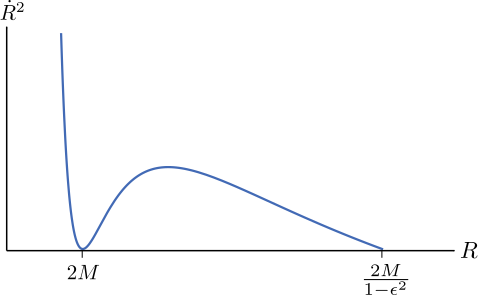
\includegraphics[width=0.7\textwidth]{Rt}
\caption{$\dot R^2$ as a function of $R$ for the massive surface particle.}
\label{fig:Rt}
\end{center}
\end{figure}

How much time $t_{2M}$ does it take the particle to reach $R=2M$ from $R=\Rmax$? Integrating~\eqref{eq:ss3}, we find
\be
t_{2M}=\int_0^{t_{2M}} dt=-\epsilon\int_{\Rmax}^{2M}dR\sfacR^{-1}\left(\frac{2M}{R}-1+\epsilon^2\right)^{-\frac12}=\infty\,!
\ee
To convince yourself that this integral is infinite, look at the contribution to the integral from the region near $R=2M$. Let $R=2M+\rho$ with $0<\rho\ll2M$ and Taylor expand in $\rho$:
\be
\bal
t_{2M}&=\mathrm{finite\,number}-\epsilon \int_\rho^0 d\rho\left(1-\frac{2M}{2M+\rho}\right)^{-1}\left(\frac{2M}{2M+\rho}-1+\epsilon^2\right)^{-\frac12}\\
&=\mathrm{finite\,number}-\epsilon \int_\rho^0 d\rho\left[\frac{2M}{\rho}+\mathcal O(\rho^0)\right].
\eal
\ee
This is infinite since the $1/\rho$ term in the integral diverges logarithmically at $0$. Hence, as far as the coordinate time $t$ is concerned, the particle never reaches the Schwarzschid radius.\\

This result seems physically rather strange. The surface of a collapsing ball of dust mysteriously slows down as it approaches $R=2M$ and never actually reaches $R=2M$. 
%This peculiar situation contributed to the initial confusion concerning the apparent ``singularity'' at $r=2M$, which was long thought to be a \textit{physical} singularity of the model, making the Schwarzschild solution to the Einstein equations an unphysical. 
However, notice that while $t$ may be a meaningful measure of time for inertial observers at $r=\infty$ ($t$ is proportional to their proper time since the metric is flat at infinity), it has no physical meaning to the infalling particle itself (or to an observer falling along with it). This should not be surprising. After all, $t$ is just a coordinate, and {\bf coordinates in general relativity have no physical meaning.}\\

\begin{figure}[t]
\begin{center}
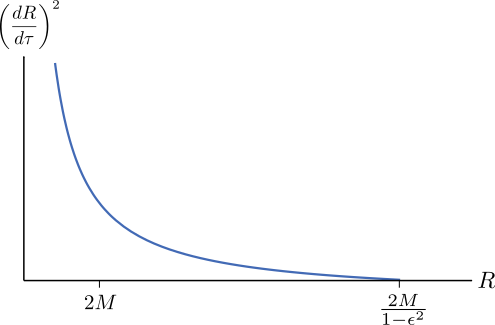
\includegraphics[width=0.7\textwidth]{Rtau}
\caption{$(dR/d\tau)^2$ as a function of $R$ for the massive surface particle.}
\label{fig:Rtau}
\end{center}
\end{figure}

So let us instead work with the proper time $\tau$ of the infalling particle. How does $R$ change as a function of $\tau$? Using~\eqref{eq:sscom} and~\eqref{eq:ss1} we find
\be
\left(\frac{dR}{d\tau}\right)^2=(1-\epsilon^2)\left(\frac{R_\mathrm{max}}{R}-1\right).\label{eq:ssRtau}
\ee
We see that nothing curious at all happens as $R\rightarrow 2M^+$. The particle (and therefore the surface of the dust ball) passes smoothly through $R=2M$. This is confirmed by the plot of $(dR/d\tau)^2$ against $R$ in Figure~\ref{fig:Rtau}.\\

Let us calculate the proper time $\tau_{2M}$ that elapses for the particle between $R=\Rmax$ and $R=2M$. Using~\eqref{eq:ssRtau}, we find \exercise
\be
\tau_{2M}=\int_{0}^{\tau_{2M}}d\tau=\int_{R_\mathrm{max}}^{2M}\left(\frac{d\tau}{dR}\right)dR=\frac{2M}{(1-\epsilon^2)^\frac32}\left(\epsilon\sqrt{1-\epsilon^2}+\arcsin\epsilon\right),
\ee
which is indeed finite. The strange behaviour near $R=2M$ has disappeared --- a first indication that the singularity in the metric at $R=2M$ is due to a pathology in the time coordinate $t$.\\

The proper time taken to reach $r=0$ is also finite:
\be
\tau_{0}=\int_{R_\mathrm{max}}^{0}\left(\frac{d\tau}{dR}\right)d\tau=\frac{\pi M}{(1-\epsilon^2)^\frac32}.
\ee
This means that the entire dust star collapses to the single point $r=0$ in a finite proper time, a first sign that there is a true singularity at $r=0$ --- a \emph{curvature singularity} --- at which physical (coordinate-independent) quantities such as $R_{\mu\nu\rho\sigma}R^{\mu\nu\rho\sigma}$ diverge.\\

While the calculations above have given us some useful insights, we have been a bit careless. We worked out the geodesics using the Schwarzschild metric, and traced them through $r=2M$, even though the metric~\eqref{eq:schwarzschild} breaks down at $r=2M$. Furthermore, for $r<2M$, the factor $\sfac$ becomes negative, which makes $t$ appear like a space-coordinate and $r$ like a time-coordinate. 
%For instance, the interval measured between two events $(t,r_0,\theta_0,\phi_0)$ and $(t+dt,r_0,\theta_0,\phi_0)$ is  \emph{spacelike} when $r<2M$. 
Statements such as ``the star collapses to $r=0$ in finite time'' then become somewhat suspect. To make our calculations sound, let us replace the coordinate system $(t,r,\theta,\phi)$ by a more suitable set of coordinates.

\subsection{Eddington-Finkelstein Coordinates}

If we want to overcome the problems encountered in the Schwarzschild coordinate system, an obvious place to start is the time-coordinate $t$. We will replace $t$ by a coordinate that is ``adapted to null geodesics''. For a null geodesic we have $ds^2=0$, which implies
\be
dt^2=\sfac^{-2} dr^2.\label{eq:nullgeo}
\ee
First, we define the radial (Regge-Wheeler) coordinate $r_*$ via
\be
dr_*^2\equiv\sfac^{-2} dr^2,\label{eq:reggewheeler}
\ee
so that null geodesics obey the simple equation $dt^2=dr_*^2$. Solving~\eqref{eq:reggewheeler} and requiring $r_*$ to be real and increasing with $r$, we obtain
\be
r_*=r+2M\ln\left(\frac{r-2M}{2M}\right).\label{eq:rstar}
\ee
The range $2M<r<\infty$ corresponds to $-\infty <r_*<\infty$, since $r_*\rightarrow-\infty$ as $r\rightarrow 2M^+$.
%\footnote{The constant in the solution to the differential equation has been fixed so that $r_*\rightarrow-\infty$ as $r\rightarrow2M^+$.} 
For this reason, $r_*$ is also known as a \emph{tortoise coordinate}: as we approach the Schwarzschild radius, $r$ changes more and more slowly with $r_*$ since $dr/dr_*\rightarrow0$.\\

The solutions $t\pm r_*=const.$ correspond to ingoing and outgoing null geodesics. Let us define a new pair of \emph{lightcone coordinates}: 
\be
\bal
u&=  t-r_*\\
v&=  t+r_*,
\eal
\ee
such that lines of constant $v$ correspond to ingoing null geodesics and lines of constant $u$ to outgoing null geodesics.\\

\subsubsection{Ingoing Eddington-Finkelstein coordinates}

We now make a coordinate transformation from $(t,r,\theta,\phi)$ to $(v,r,\theta,\phi)$, i.e. we replace $t$ by the coordinate $v$ that labels ingoing radial null lines. The coordinates $(v,r,\theta,\phi)$ are called \emph{ingoing Eddington-Finkelstein (IEF) coordinates} and the line-element in $IEF$ coordinates reads~\exercise
\be
ds^2=-\sfac dv^2+2dvdr+r^2d\Omega_2^2.\label{eq:ef1}
\ee
This metric is perfectly regular at $r=2M$ (i.e. it is non-degenerate: $\det g\munu\neq0$).
%[[MB1: state why it should be non-degenerate]]. 
In fact, it is fine \emph{everywhere} except at $r=0$. We may therefore extend the range of $r$ across $r=2M$ to all $r>0$ (you can easily check that~\eqref{eq:ef1} is a solution to the vacuum Einstein equations $R_{\mu\nu}=0$ for all $r>0$). We can see clearly now that there is nothing peculiar about $r=2M$; there is nothing going on in the local physics that would tell you that you are approaching or passing through the surface $r=2M$. The original coordinates $(t,r,\theta,\phi)$ were simply not suitable to describe the spacetime region beyond $r=2M$ due to their bad behaviour there.\\
%\footnote{The following analogy may be illustrative. Imagine someone describes to you a metric space parametrised by polar coordinates $(r,\theta)$ where $r>0$ and $0\leq\theta<2\pi$, and on which the metric is given by $ds^2=dr^2+r^2d\theta^2$. Note that $r=0$ is \emph{not} a point in this space, since the metric is ill-defined (non-degenerate) there. You then happen to find a convenient new set of coordinates $(x,y)=(r\cos\theta,r\sin\theta)$, where $(x,y)\in\mathbb R^2\setminus(0,0)$ (since $r=0$ is not included). In these coordinates the metric takes the form $ds^2=dx^2+dy^2$. Now, this metric is perfectly regular at the point $(x,y)=(0,0)$. So you decide to \emph{extend} your original space by adding to it the point $(x,y)=(0,0)$. You realise that there is nothing geometrically ``weird'' about the point $r=0$, even though it certainly looked like it in your original coordinate system: polar coordinates were simply bad coordinates at $r=0$.}\\

%[[MB1: include statements about ``local physics'' somewhere]].\\

Figure~\ref{fig:ief} shows radial ingoing ($v=const.$) and outgoing ($u=const.$) null geodesics in the $IEF$ metric. Notice how the lightcones tip over as we cross the Schwarzschild radius: while ``outgoing'' photons that start off oustide the horizon eventually escape to infinity, ``outgoing'' photons emitted at $r=2M$ \emph{remain} at $r=2M$ forever.\footnote{This reveals one at first perhaps counter-intuitive aspect of the horizon, which we will see in more detail in later sections: the surface $r=2M$ is a \emph{null} surface (null geodesics travel along it), even though it is a surface of constant $r$.} ``Outgoing'' photons emitted at $r<2M$ stay within $r<2M$ and fall towards $r=0$. As they reach $r=2M$, their geodesics become parallel to ingoing null geodesics. \\



\begin{figure}[t]
\begin{center}
\includegraphics[width=\textwidth]{IEF}
\caption{Ingoing (dashed red) and outgoing (solid blue) null geodesics in $IEF$ coordinates for $M=1$. The horizon at $r=2M$ is highlighted in black.}
\label{fig:ief}
\end{center}
\end{figure}

We call the surface $r=2M$ (a two-sphere in $3+1$ dimensions) the \emph{event horizon} and the region $r<2M$ the \emph{black hole}. The surface dust particle is massive, so its worldline must lie between ingoing and outgoing null geodesics (inside the lightcone). As you can see in Figure~\ref{fig:ief}, this means that the particle must eventually hit $r=0$. Furthermore, no signal from an event inside the event horizon can ever escape the black hole to reach an observer at $r>2M$. \\



From Figure~\ref{fig:ief} we can also get an idea how someone hovering at a fixed radius $r>2M$ outside the black hole will perceive the infalling matter as it falls across the horizon. Imagine a signal being transmitted from the surface of the dust ball at a constant rate. Due to the bending of the lightcones in the vicinity of the horizon, the signals reaching the observer will become sparser and sparser as the surface approaches $r=2M$. If we think of these signals as electromagnetic radiation, i.e. light, then the light is shifted toward the lower (i.e. red) end of the spectrum, and the signal received by the distant observer becomes redder and redder until it eventually disappears.\\

%On a more practical note: since \emph{every} timelike curve hits $r=0$ eventually, and proper time is maximised on timelike geodesics, your best strategy if you ever find yourself falling across a black hole horizon is to \emph{fall freely}. 
%[[MB1: Explain]].\\

\subsubsection{Outgoing Eddington-Finkelstein coordinates}

In the previous section, we made a coordinate transformation by replacing $t$ by $v$. Another obvious possibility is to use the outgoing EF coordinate $u=t-r_*$ instead. This leads to \emph{outgoing Eddington-Finkelstein (OEF)} coordinates $(u,r,\theta,\phi)$.\\

The metric in $OEF$ coordinates is given by
\be
ds^2=\sfac du^2-2dudr+r^2d\Omega_2^2.\label{eq:ef2}
\ee
Note the similarity between~\eqref{eq:ef1} and~\eqref{eq:ef2}: the only difference is the sign of the cross-term. However, the physical picture of the spacetime described by the line-element~\eqref{eq:ef2} turns out to be very different. To see this, let us consider again ``ingoing'' ($v=const.$) and ``outgoing'' ($u=const.$) null geodesics. They are depicted in Figure~\ref{fig:oef}, where we have defined the $OEF$ time $t_*=u+r_*$. ``Ingoing'' photons emitted at $r>2M$ or $r<2M$ never cross $r=2M$: they approach $r=2M$ and hover the horizon forever. Conversely, all outgoing null geodesics escape to infinity. Looking at the lightcones, we see that everything inside $r=2M$ is ejected. The interior region $r<2M$ is therefore called a \emph{white hole} and $r=2M$ the white hole horizon. It is the exact time reversal of a black hole (you can see this by turning Figure~\ref{fig:ief} upside down and comparing it with Figure~\ref{fig:oef}). \\

What happens in the spacetime described by $OEF$ coordinates is clearly very different from what happens in the spacetime described by $IEF$ coordinates. This may seem contradictory, since both are obtained by coordinate transformations from the original Schwarzschild spacetime. We will learn how to make sense of this apparent contradiction by introducing yet another coordinate system.

\begin{figure}[t]
\begin{center}
\includegraphics[width=\textwidth]{OEF}
\caption{Ingoing (dashed red) and outgoing (solid blue) null geodesics in the $OEF$ metric for $M=1$. The horizon at $r=2M$ is highlighted in black.}
\label{fig:oef}
\end{center}
\end{figure}

\subsection{Kruskal-Szekeres Coordinates}\label{sec:KScoords}

First, change coordinates to $(u,v,\theta,\phi)$, replacing both Schwarzschild coordinates $r$ and $t$ by $u=t-r_*$ and $v=t+r_*$ (where $r_*$ is the function of $r$ defined in~\eqref{eq:rstar}). The metric then reads
\be
ds^2=-\sfac dudv+r^2d\Omega_2^2,
\ee
where $r=r(u,v)$ can be given in terms of $u$ and $v$ via~\eqref{eq:rstar} and $r_*=(v-u)/2$. This metric has a coordinate singularity at $r=2M$, so it is only defined for $r\neq2M$. To remove the singularity, we define a new pair of coordinates $U$ and $V$ in the region $r>2M$ by
\be
U=-\exp\left(-\frac{u}{4M}\right)\qquad\mand\qquad
V=\exp\left(\frac{v}{4M}\right).\label{eq:UV}
\ee
Note that $U<0$ and $V>0$ for all values of $r$. The coordinates $(U,V,\theta,\phi)$ are called \emph{Kruskal-Szekeres (KS) coordinates}. The Schwarzschild metric in KS coordinates is \textsf{(exercise)}:
\be
ds^2=-\frac{32M^3}{r}\exp\left(-\frac{r}{2M}\right)dUdV+r^2d\Omega_2^2,\label{eq:KS}
\ee
where $r=r(U,V)$ is defined in terms of $U$ and $V$ by the implicit equation\linebreak$UV=-\lbr\frac{r-2M}{2M}\rbr\exp\lbr\frac{r}{2M}\rbr$.\footnote{We can write $r$ explicitly as $r(U,V)=2M\lsq1+W\lbr-UV/e\rbr\rsq$ where $e$ is Euler's constant and $W$ stands for the \href{http://en.wikipedia.org/wiki/Lambert_W_function}{Lambert $W$-function}.}\\

This metric is well-defined for $r=2M$ and indeed for all $r>0$. Notice that for $r<2M$, we have $UV>0$, which is incompatible with~\eqref{eq:UV}. Let us therefore~\emph{forget} the initial definitions of $U$ and $V$ in terms of the Schwarzschild coordinates for now (much like we did for $u$ and $v$ when we went from Schwarzschild to Eddington-Finkelstein coordinates), and instead investigate the new spacetime with metric~\eqref{eq:KS} an extended coordinate ranges $-\infty<U,V<\infty$. \\

\begin{figure}[t]
\begin{center}
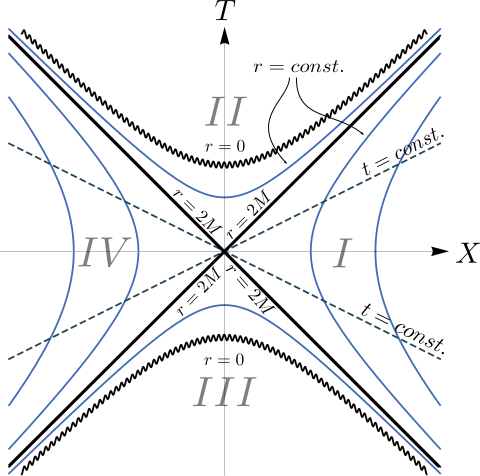
\includegraphics[width=0.6\textwidth]{ks}
\caption{Kruskal spacetime. Each point represents a $2-$sphere of radius $r(T,X)$. The black lines at $45^\circ$ correspond to $r=2M$. The singularity $r=0$ is represented by a wavy line. Solid blue hyperbolae correspond to $r=const.$ surfaces and straight dashed lines correspond to $t=const.$ surfaces.}
\label{fig:KS}
\end{center}
\end{figure}

Figure~\ref{fig:KS} is a picture of the spacetime described by the KS metric. Since null lines are conventionally plotted at $45^\circ$, we define time and space coordinates $T=U+V$ and $X=T-V$, which label the vertical and horizontal axes in the figure. The $U$ and $V$ axes are then at $45^\circ$ to the $T$ and $X$ axes. At the horizon $r=2M$, we have $UV=0$, which means either $U=0$ or $V=0$. This corresponds to the solid diagonals. The  singularity $r=0$ corresponds to the (two branches of the) hyperbola described by $UV=1$, which is represented by a wavy line (singularities will always be represented by wavy lines). In general, surfaces of $r=const.$ correspond to hyperbolae $UV=const.$ with $UV<1$, as shown in blue on the diagram. Spatial sections with $t=const.$ have $U/V=const.$ and $|U/V|<1$, which corresponds to straight lines through the origin with gradient between $-1$ and $1$. Finally, ingoing and outgoing null geodesics are respectively given by $U=const.$ and $V=const.$ \\

We can now see the relation between the different coordinate systems. The original Schwarzschild coordinates $(t,r,\theta,\phi)$ only cover region $I$. When we changed to $IEF$ and $OEF$ coordinates, we extended our spacetime to regions $II$ and $III$, respectively. There is a new region that we only see in KS coordinates, region $IV$. This region is a mirror image of region $I$, which can be seen by defining
\be
U=\exp\left(-\frac{u}{4M}\right)\qquad\mand\qquad
V=-\exp\left(\frac{v}{4M}\right)\label{eq:UV2}
\ee
on region $IV$ and noting that the metric~\eqref{eq:KS} will be of the same form as the Schwarzschild metric. (The proper statement is that region $IV$ is \emph{isometric} to region $I$. In general relativity, two spacetimes or regions of spacetime that are isometric are physically identical.)\\
%\footnote{The process of extending a spacetime in this way is also called \emph{analytic continuation}. The reason for the name is that we can ``access'' some of the extended regions that are hidden in a given coordinate patch by letting coordinates take on complex values. For example, in Schwarzschild coordinates that only cover region $I$, we could access region $IV$ by letting $t\rightarrow t+4M\pi i$ (which turns~\eqref{eq:UV} into~\eqref{eq:UV2}).} \\

The geometry of spatial sections is also worth a closer look. Consider a slice with $t=const. \iff T/X=const.$ On Figure~\ref{fig:KS}, it corresponds to a straight line through the point $(T,X)=(0,0)\iff r=2M$, where regions $I$ and $IV$ attach to each other. In both regions the metric on the slice is given by
\be
ds^2=\sfac^{-1}dr^2+r^2d\Omega_2^2\label{eq:constantTmetric}
\ee
and in both regions $r$ increases from $2M$ to $\infty$. For large $r$, we have $\sfac\rightarrow1$ and so the geometry becomes Euclidean. As we approach $r=2M$, i.e. the centre in Figure~\ref{fig:KS}, the metric~\eqref{eq:constantTmetric} starts to deviate from the Euclidean metric. What is the geometry near $r=2M$? Since we cannot draw a three-dimensional surface, let us suppress one angular coordinate by setting $\theta$ to its equatorial value $\theta=\frac\pi2$. Then the metric is $ds^2=\sfac^{-1}dr^2+r^2d\phi^2$. 
It is not hard to show \exercise~that this is just the metric on a so-called quartic surface $x^2+y^2=(z^2/8M+2M)^2$ embedded in three-dimensional Euclidean space $\mathbb E^3$ with cartesian coordinates $x,y,z$.\footnote{Hint: Recall that the metric on $\mathbb E^3$ is $ds^2=dx^2+dy^2+dz^2$. Consider the surface parametrised by $x=r\cos\phi$, $y=r\sin\phi$ and $z=\sqrt{8M(r-2M)}$, show that it satisfies the quartic equation above and find the metric induced on it. For an illustration see \href{http://wolfr.am/WIRjK3}{http://wolfr.am/WIRjK3}.} 
The geometry is shown in Figure~\ref{fig:ERbridge}, where two identical copies of the surface have been attached to each other at the circle $r=2M$. One side corresponds to region $I$ and the other side to region $IV$. This is known as the \emph{Einstein-Rosen bridge}, which is one example of a \emph{wormhole}. Note that no observer can ever cross the wormhole, as you can see clearly in the Kruskal diagram (and, further along in the lectures, in the Penrose diagram for Kruskal space): in order to cross the wormhole from region $I$ to $IV$ or vice-versa, the trajectory of the observer would have to be spacelike somewhere. \\

\begin{figure}[t!]
\begin{center}
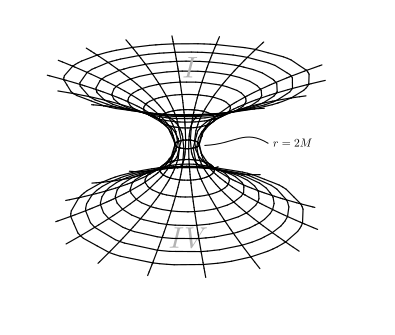
\includegraphics[width=0.5\textwidth]{wormhole}
\caption{The Einstein-Rosen bridge with one spatial dimension suppressed. Each circle represents a two-sphere in the three-dimensional analogue.}
\label{fig:ERbridge}
\end{center}
\end{figure}

We can also get an intuitive sense for the strange sign change that appears in the original Schwarzschild metric~\eqref{eq:schwarzschild} between $r>2M$ and $r<2M$, which makes $r$ appear like a time coordinate when $r<2M$. Indeed, if $r=0$ were just a ``position in space'', as one might naively think of it, it would seem that one could simply avoid it by navigating around it. In Figure~\ref{fig:KS}, we see that for anyone who has fallen across the horizon, the singularity $r=0$ is \emph{not} a position in space --- it becomes a \emph{moment of time}, as unavoidable as 9am tomorrow morning.\\

Finally, we can justify in retrospect some of the coordinate extensions (analytic continuations) that we performed rather ad-hoc in the last sections. For example, consider the extension from region $I$ covered by Schwarzschild coordinates to regions $I+II$ covered by $IEF$ coordinates. The original coordinate system with time coordinate $-\infty<t<\infty$ covers region $I$ only. If we think of region $I$ as a physical spacetime in its own right, then a particle will hit a ``boundary'' ($r=2M$) in finite proper time $\tau_{2M}$. In light of this, it seems physically quite reasonable to work instead with the spacetime $I+II$ obtained by extending the original coordinate system, where this artificial boundary disappears.

\subsection{Penrose Diagrams}

In this section we introduce a useful way of representing the causal structure of an infinite spacetime on a finite piece of paper. This involves performing a \emph{conformal transformation} on the metric:\\

\begin{definition} 
A \emph{conformal transformation} is a map from a spacetime $(M,g)$ to a spacetime $(M,\tilde g)$ such that
$$
\tilde g_{\mu\nu}(x)=\Lambda(x)^2g_{\mu\nu}(x)
$$
where $\Lambda(x)$ is a smooth function of the spacetime coordinates and $\Lambda(x)\neq0\;\forall\;x$.\\
\end{definition}

Conformal transformations preserve the causal structure of a spacetime. To see this, consider a vector $V^\mu$ on $M$. Then it follows from $\Lambda(x)^2>0$ that
\be
\bal
g_{\mu\nu}V^\mu V^\nu >0 &\iff \tilde g_{\mu\nu}V^\mu V^\nu >0\\
g_{\mu\nu}V^\mu V^\nu =0 &\iff \tilde g_{\mu\nu}V^\mu V^\nu =0\\
g_{\mu\nu}V^\mu V^\nu <0 &\iff \tilde g_{\mu\nu}V^\mu V^\nu <0.
\eal
\ee
Hence, curves that are timelike/null/spacelike with respect to $g$ are timelike/null/ spacelike with respect to $\tilde g$. 
%In particular, a curve is causal (has non-spacelike tangent vector everywhere) with respect to $g$ if and only if it is causal with respect to $\tilde g$. 
Furthermore, by consequence of the second line, null geodesics for $g$ correspond to null geodesics for $\tilde g$ (whereas timelike/spacelike geodesics for $g$ are \emph{not} necessarily geodesics for $\tilde g$).\\

The idea of a Penrose diagram is this. First, we use a coordinate transformation on the spacetime $(M,g)$ to bring ``infinity'' to a finite coordinate distance, so that we can draw the entire spacetime on a sheet of paper. The metric will typically diverge as we approach the ``points at infinity'', i.e. the edges of the finite diagram. To remedy this, we perform a conformal transformation on $g$ to obtain a new metric $\tilde g$ that is regular on the edges. Then $(M,\tilde g)$ is a good representation of the original spacetime $(M,g)$ insofar that it has exactly the same causal structure. It is customary to add the points at infinity to $M$ to form a new manifold $\tilde M$. The resulting spacetime $(\tilde M,\tilde g)$ is what is called the \emph{conformal compactification} of $(M,g)$.\\

Note that the curvature tensors are in general not preserved under conformal transformations, e.g. $\tilde R^\mu_{\nu\rho\sigma}\neq R^\mu_{\nu\rho\sigma}$, $\tilde R\neq R$ etc. In that sense, the conformally compactified spacetime $(\tilde M,\tilde g)$ is unphysical: it provides a good representation of the causal structure of the physical spacetime $(M,g)$, but it should otherwise not be viewed as a picture of what is going on (for example, as noted above, the geodesics of massive test particles in $(\tilde M, \tilde g)$ do not correspond to geodesics of massive test particles in $(M,g)$).\\
%This reflects the fact that the causal structure does not encode everything physical about a metric. However, we will see later on that the causal structure encodes \emph{almost} everything (in $4$ dimension it gives you $9/10$ components of the metric).\\

\subsubsection{Example 1: Minkowski space in $1+1$ dimensions} The two-dimensional Minkowski metric is given by
\be
ds^2=-dt^2+dx^2
\ee
where $-\infty<t,x<\infty$. We introduce light-cone coordinates $u=t-x$ and $v=t+x$, in which the metric $g\munu$ takes the simple form
\be
ds^2=-dudv.
\ee
Now, to shrink ``infinity'' down to a finite coordinate distance, we define a new set of coordinates via 
\be
\bal
u&=\tan\tilde u\\
v&=\tan\tilde v.\label{eq:uvtilde}
\eal
\ee These coordinates indeed have a finite range $-\frac\pi2<\tilde u,\tilde v<\frac\pi2$ (the range is open since points with $u,v=\tan(\pm\frac\pi2)=\pm\infty$ are \emph{not} points in spacetime). The line-element in terms of $\tilde u$ and $\tilde v$ is
\be
ds^2=-\frac{1}{\lbr\cos\tilde u\cos\tilde v\rbr^{2}}d\tilde u d\tilde v.
\ee
It diverges as $u,v\rightarrow\pm\infty\iff\tilde u,\tilde v\rightarrow \pm\frac\pi2$. Define a new metric $\tilde g_{\mu\nu}$ through a conformal transformation on $g\munu$:
\be
d\tilde s^2=\lbr\cos\tilde u\cos\tilde v\rbr^{2} ds^2=-d\tilde u d\tilde v.
\ee
This metric is regular at the points at infinity where either $\tilde u$ or $\tilde v$ are equal to $\pm\frac\pi2$ and we can now add those points to the spacetime. The resulting spacetime $(\tilde M,\tilde g)$ is the conformal compactification of $(M,g)$. Both spacetimes are shown in $(\tilde u,\tilde v)$ coordinates in Figure~\ref{fig:cp2dmink}.\\

\begin{figure}[t]
\begin{center}
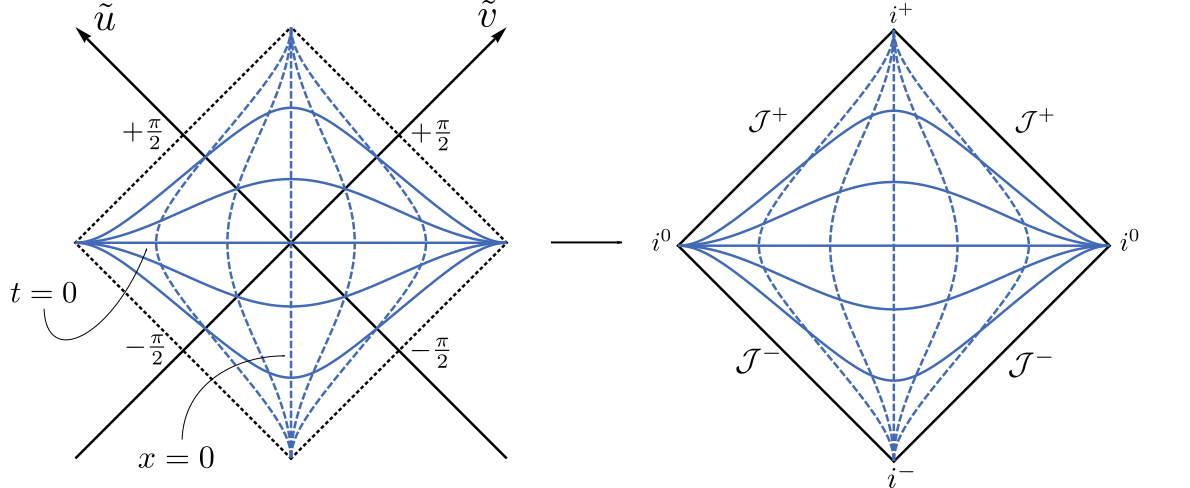
\includegraphics[width=\textwidth]{penrosemink}
\caption{\textbf{Left:} Minkowski space $(M, g)$ in $(\tilde u,\tilde v)$ coordinates. The boundaries $\tilde u,\tilde v=\pm\frac\pi2$ are not part of $M$ and $g$ diverges there. Some timelike and spacelike geodesics of $g$ have been included: lines with $r=const.$ are represented by dashed curves and lines with $t=const.$ are represented by solid curves. \textbf{Right:} The Penrose diagram of conformally compactified Minkowski space $(\tilde M,\tilde g)$, with future/past timelike infinity $i^\pm$, future/past null infinity $\scri^\pm$ and spacelike infinity $i^0$. The timelike and spacelike geodesics of Minkowski space are clearly not all geodesics for $(\tilde M,\tilde g)$, since $\tilde g$ is flat in $(\tilde u,\tilde v)$ coordinates.}
\label{fig:cp2dmink}
\end{center}
\end{figure}

The two points $(\tilde u,\tilde v)=(\frac\pi2,\frac\pi2)$ and $(-\frac\pi2,-\frac\pi2)$ are denoted by $i^\pm$. All future (past) directed timelike curves end up at $i^+$ ($i^-$), so we refer to $i^+$ ($i^-$) as \emph{future (past) timelike infinity}. Future directed null geodesics either end up at $\tilde v=\frac\pi2$ with constant $|\tilde u|<\frac\pi2$ or  at $\tilde u=\frac\pi2$ with constant $|\tilde v|<\frac\pi2$. This set of points is denoted by $\scri^+$ (``scri-plus'') and referred to as \emph{future null infinity}. An analogous definition holds for past null infinity $\scri^-$ (``scri-minus''). Finally, \emph{spacelike infinity} $i^0$ denotes the set of endpoints of spacelike geodesics, which corresponds here to $(\tilde u,\tilde v)=(\frac\pi2,-\frac\pi2)$ and $(\tilde u,\tilde v)=(-\frac\pi2,\frac\pi2)$.\\
%it is just a flat diamond. Null geodesics in this diamond correspond to null geodesics in Minkowski space.\\

\subsubsection{Example 2: Minkowski space in $3+1$ dimensions} The four-dimensional Minkowski metric
\be
ds^2=-dt^2+dx^2+dy^2+dz^2
\ee
can be written in terms of spherical polar coordinates $(t,r,\theta,\phi)$ by choosing an arbitrary point as the origin, say $x=y=z=0$. We then have 
\be
ds^2=-dt^2+dr^2+r^2d\Omega_2^2
\ee
where $d\Omega_2^2$ is the round metric on the $2$-sphere. Define light-cone coordinates $u=t-r$ and $v=t+r$ and perform the same transformation~\eqref{eq:uvtilde} as above to bring infinity to finite coordinate distance. The only difference to the previous analysis is that since $r\geq0$, we have the additional constraint $u\leq v\iff\tilde u\leq \tilde v$. The metric in $(\tilde u,\tilde v,\phi,\theta)$ coordinates reads
\be
ds^2=-\frac{1}{\lbr2\cos\tilde u\cos\tilde v\rbr^{2}}\lsq-4d\tilde u d\tilde v+\sin^2\lbr\tilde v-\tilde u\rbr d\Omega_2^2\rsq
\ee
and its conformal compactification corresponds to the spacetime $(\tilde M, \tilde g)$ with metric
\be
d\tilde s^2=\lbr\cos\tilde u\cos\tilde v\rbr^{2}ds^2=-4d\tilde u d\tilde v+\sin^2\lbr\tilde v-\tilde u\rbr d\Omega_2^2.
\ee
and extended coordinate ranges $-\pi/2\leq\tilde u,\tilde v\leq\pi/2$. On the Penrose diagram of $1+1$ dimensional Minkowski space in Figure~\ref{fig:cp2dmink}, $\tilde u\leq \tilde v$ implies that we only include the part that lies to the right of the vertical line $x=0$. The resulting diagram for the $3+1$ space is shown in Figure~\ref{fig:cpmink4draw}.  Every point on the diagram represents a two-sphere of radius $\sin(\tilde v-\tilde u)$. \\

\begin{figure}[t]
  \begin{center}
    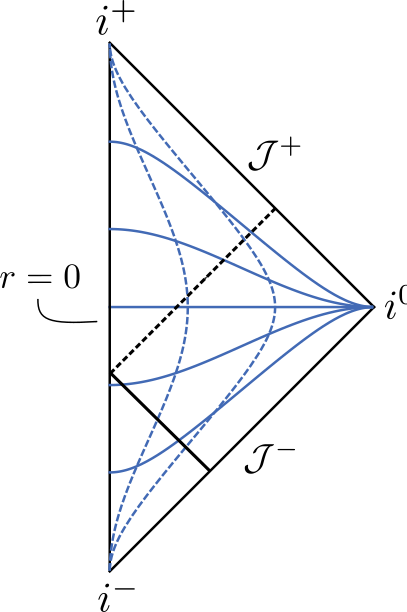
\includegraphics[scale=0.4]{cpmink4draw}\hspace{0.2\textwidth}\includegraphics[width=0.25\textwidth]{esumink}
  \end{center}
  \caption{\textbf{Left:} The Penrose diagram of $3+1$ dimensional Minkowski space with some lines of constant $r$ and $t$. Each point represents a $2-$sphere. As the null geodesic shown passes through $r=0$, it emerges on another copy of the Penrose diagram whose points represent the antipodes on the two-spheres. \textbf{Right:} The conformal compactification drawn as a portion of the Einstein static universe with the same null geodesic.}
  \label{fig:cpmink4draw}
\end{figure}

There exists a somewhat more illustrative way to picture the conformal compactification. Define $\tilde T=\tilde v+\tilde u$ and $\chi=\tilde v-\tilde u$. The coordinate ranges are then \exercise\, $-\pi<\tilde T<\pi$ and $0<\chi<\pi$ and the metric reads
\be
d\tilde s^2=-d\tilde T^2+d\chi^2+\sin^2\chi d\Omega_2^2.\label{eq:ESU}
\ee
The spatial part $d\chi^2+\sin^2\chi d\Omega_2^2$ of this metric is just the round metric of a three-sphere $S^3$ parametrised by polar coordinates $(\chi,\theta,\phi)$. The spacetime~\eqref{eq:ESU} therefore represents a static universe with spherical spatial slices, which corresponds to a finite portion of the \emph{Einstein static universe (ESU)} whose topology is $\mathbb R\times S^3$. This is shown in Figure~\ref{fig:cpmink4draw}, and the Penrose diagram corresponds to that part of the region wrapped around the cylinder facing out of the page. \\

\subsubsection{Example 3: Rindler space in ${1+1}$ dimensions} \label{sec:cprindler}

Rindler space is a subregion of Minkowski space associated with observers eternally accelerated at a constant rate. The worldlines of these ``Rindler observers'' (accelerating in the positive $x$-direction) is given by the hyperbolae $x_\mu x^\mu=-t^2+x^2=\xi^2$. You can check \textsf{(exercise)} that the $4$-acceleration $a^\mu=d^2x^\mu/d\tau^2$ along this worldline is indeed constant: $a_\mu a^\mu=1/\xi^2$.\\

\begin{figure}[t]
\begin{center}
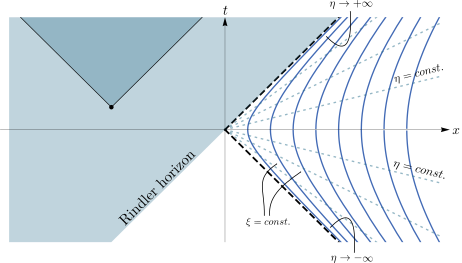
\includegraphics[width=0.85\textwidth]{accelerated}
\caption{Eternally accelerating observers in Minkowski space. Their worldlines are shown in blue and labelled by $\xi$. Events in the shaded region such as the black dot are hidden to them. The Rindler horizon is the boundary between the shaded and unshaded regions. Rindler space corresponds to the right wedge outlined by the dashed black null lines. The straight dotted lines are lines of constant Rindler time $\eta$.}
\label{fig:accelerated}
\end{center}
\end{figure}

Consider the one-parameter family of Rindler observers depicted in Figure~\ref{fig:accelerated}. The region $x\leq t$ is forever hidden to them, which makes the line $x=t$ a horizon to these observers.\footnote{This horizon is different from the event horizon in the Schwarzschild black hole spacetime, since the Schwarzschild horizon is observer/frame-independent, while the horizon here is associated with a family of special observers/frames.}\emph{Rindler space} corresponds to the right wedge $x>|t|$ foliated by the worldlines of the accelerated observers in Figure~\ref{fig:accelerated}. To obtain the Rindler metric, we introduce a new set of space and time coordinates $\xi$ and $\eta$ in the subregion $x>|t|$ of Minkowski space. As space coordinate we use $\xi$, which labels the hyperbolic worldlines $x^2-t^2=\xi^2$. As time coordinate we use the proper time $\eta=\mathrm{tanh}^{-1}(t/x)$ measured by a Rindler observer, synchronised such that $\eta=0$ when the observer passes the $x$-axis. The relation to Cartesian coordinates is
\be
x=\xi\cosh\eta \mand t=\xi\sinh\eta
\ee
and the coordinate ranges are $0<\xi<\infty$ and $-\infty<\eta<\infty$.
The Minkowski metric in $(\eta,\xi)$ coordinates is
\be
ds^2=-\xi^2d\eta^2+d\xi^2.
\ee
The proper time measured by an accelerated observer --- i.e. a stationary ($\xi=const.$) observer in Rindler coordinates --- is $\tau=\xi\eta$. Since Rindler space is a subregion of Minkowski space, the Penrose diagram is just a piece of Figure~\ref{fig:cp2dmink}, as shown in Figure~\ref{fig:cp2drindler}. \\

\begin{figure}[t!]
\begin{center}
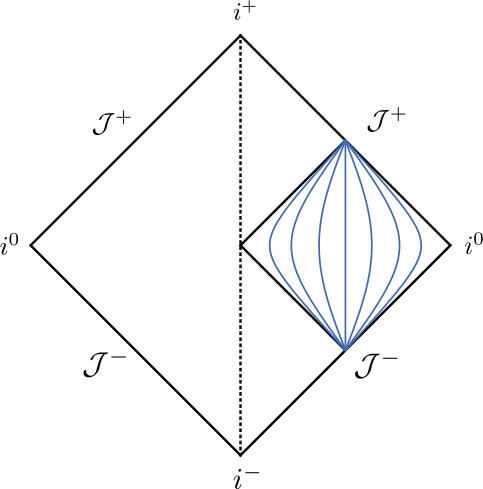
\includegraphics[width=0.4\textwidth]{penroserindler}
\caption{The Penrose diagram for $1+1$ dimensional Rindler space, seen as a portion of Minkowski space. Some accelerated worldlines (curves of constant $\xi$) have been drawn for $\xi=\frac29,\frac25,\frac23,1,\frac32,\frac52,\frac92$. Note that all of the worldlines represent observers accelerating in the postitive $x-$direction, even though they appear to bend toward the right for $\xi>1$. This distortion is a side effect of the coordinate transformation $(u,v)\rightarrow(\tilde u,\tilde v)$.}
\label{fig:cp2drindler}
\end{center}
\end{figure}

\subsubsection{Example 4: Kruskal space in $3+1$ dimensions}
Recall the Kruskal metric~\eqref{eq:KS}:
$$
ds^2=-\frac{32M^3}{r}\exp\left(-\frac{r}{2M}\right)dUdV+r^2d\Omega_2^2.
$$
Define a new set of null coordinates via $U=\tan\tilde U$ and $V=\tan\tilde V$, such that $-\frac\pi2<\tilde U,\tilde V<\frac\pi2$. Then the line-element becomes
\be
\!\!ds^2=(2\cos\tilde U\cos\tilde V)^{-2}\left[-4\frac{32M^3}r \exp\left(-\frac{r}{2M}\right) d\tilde U d\tilde V+r^2\cos^2\tilde U\cos^2\tilde V d\Omega_2^2\right]
\ee
We perform the usual conformal transformation, which leaves us with
\be
\bal
d\tilde s^2&=(2\cos\tilde U\cos\tilde V)^{2}ds^2\\
&=-4\frac{32M^3}r \exp\left(-\frac{r}{2M}\right)d\tilde U d\tilde V+r^2\cos^2\tilde U\cos^2\tilde V d\Omega_2^2,
\eal
\ee
and we add the points at infinity. The curvature singularity $UV=1$ now corresponds to
\be
\tan\tilde U\tan\tilde V=1\iff\sin\tilde U\sin\tilde V=\cos\tilde U\cos\tilde V\iff\cos(\tilde U+\tilde V)=0
\ee
which implies $\tilde U+\tilde V=\pm\frac\pi2$, or $\tilde T=\pm\frac\pi4$ if we define $\tilde T$ and $\tilde X$ through $\tilde U=\tilde T-\tilde X$ and $\tilde V=\tilde T+\tilde X$ in analogy to section~\ref{sec:KScoords}. The Penrose diagram including the points at infinity and the singularity is shown in Figure~\ref{fig:cpkruskal}. Also shown is the curve corresponding to the surface of a collapsing star. If we only keep the region exterior to the surface, we obtain the Penrose diagram for the collapsing star on the right. The interior of the star is excluded since the stress-energy tensor is non-zero there and spacetime is not described by the Schwarzschild metric. Therefore, regions $I$ and $III$ are the only regions of Kruskal spacetime relevant to the description of a black hole formed through stellar collapse.\\

%Note that $u$ and $\tilde U$ break down as a coordinates in the black hole region whereas $v$ and $\tilde V$ break down in the white hole region. Far from the black hole, $\Delta u\approx \Delta t=\Delta\tau$ is a good measure of the proper time for a distant inertial observer. This is shown in Figure~\ref{fig:cpkruskal}. [[MB1: finish]]

\begin{figure}[t!]
\begin{center}
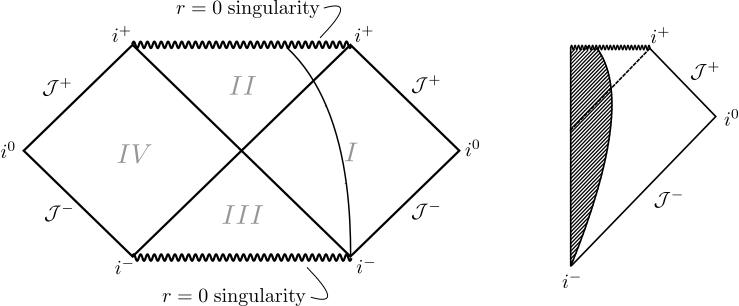
\includegraphics[width=\textwidth]{cpkruskalcombo}
\caption{\textbf{Left:} The Penrose diagram for Kruskal space. The possible trajectory of the surface of a collapsing star is shown --- the region to the left of the curve corresponds to the interior of the star, where spacetime is not described by the Kruskal metric. \textbf{Right:} The Penrose diagram for a collapsing star. The curved line represents the surface and the shaded region corresponds to the interior of the star. The horizon corresponds to the dashed line.}
\label{fig:cpkruskal}
\end{center}
\end{figure}

\subsubsection{Example 5: de Sitter space in $3+1$ dimensions}

The de Sitter metric is a solution of the Einstein equations in the presence of a positive cosmological constant $\Lambda>0$:  
\be
R\munu-\frac12Rg\munu+\Lambda g\munu=0.\label{eq:einsteinds}
\ee
It corresponds to a universe with uniform positive energy density and negative pressure. To see this, note that~\eqref{eq:einsteinds} can be interpreted as the Einstein equations in the presence of an energy momentum tensor
\be
R\munu-\frac12Rg\munu=T\munu
\ee
with $T\munu=-\Lambda g\munu$, which implies positive energy density $T_{00}=\Lambda$ and negative uniform pressure $T_{ii}=-\Lambda$ for $i=1,2,3$.\\

%de Sitter space is interesting as a spacetime due to its applications in cosmology. For one, it is a good model for a universe undergoing an inflationary expansion, which is a . It is interesting now because there is evidence that the current expansion of the universe is expanding, which corresponds to an approximately de Sitter universe. of particular interest for two reasons. to the observation that our current universe is expanding at an accelerated rate, and due to its relevance to scenarios in which the universe underwent an exponential expansion in its earliest phases. [[MB1: REPHRASE]]. MENTION ADS AND STRING THEORY.\\

de Sitter space admits a number of different coordinate systems, some of which cover the whole space and some of which cover only part of it. The geometry of spatial sections in these coordinates can also vary (closed, open, flat). One convenient set of coordinates are closed global coordinates $(t,\chi,\theta,\phi)$ in which the line-element reads
\be
ds^2=-dt^2+a^2\cosh^2(t/a)d\Omega_3^2,\label{eq:dsmetric}
\ee
corresponding to a spacetime whose spatial sections are three-spheres with a time-dependent radius $a\cosh(t/a)$.\\

The best way to picture de Sitter space is as a hyperboloid embdedded in Minkowski space of one dimension higher (so $3+1$ dimensional de Sitter space is a hyperboloid in $4+1$ dimensional Minkowski space). Since our illustrations are restricted to three dimensions, let us suppress two of the angular coordinates by setting $\chi=\theta=\frac\pi2$. In that case, spatial cross sections are circles instead of three-spheres and $d\Omega_3^2\rightarrow d\phi^2$. To see that this two-dimensional de Sitter space is a hyperboloid embedded in three-dimensional Minkowski space, consider the surface parametrised by $T=a\sinh(t/a)$, $X=a\cosh(t/a)\cos\phi$ and $Y=a\cosh(t/a)\sin\phi$, where $T,X,Y$ are Cartesian coordinates in Minkowski space. Then it is easy to check that the embedding $2+1$ dimensional Minkowski metric $ds^2=-dT^2+dX^2+dY^2$ reproduces~\eqref{eq:dsmetric} and furthermore that de Sitter space satisfies the equation of a hyperboloid: $-T^2+X^2+Y^2=a^2$. This is shown in Figure~\ref{fig:dshyper}.\\

\begin{figure}[t]
\begin{center}
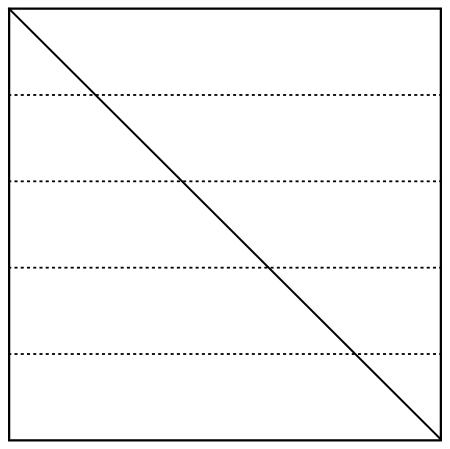
\includegraphics[width=0.9\textwidth]{cpdesittercombo}
\caption{\textbf{Left:} The $1+1$ dimensional de Sitter hyperboloid embedded in $2+1$ dimensional Minkowski space. Some curves of constant $\theta$ and $t$ are shown. \textbf{Right:} The Penrose diagram of de Sitter space. Dotted lines are lines of constant $\eta$. The diagonal line is the de Sitter horizon for a comoving observer at the north pole $\chi=0$.}
\label{fig:dshyper}
\end{center}
\end{figure}

To construct the Penrose diagram of de Sitter space we pull out the factor of $a^2\cosh^2(t/a)$ in the metric~\eqref{eq:dsmetric}:
\be
ds^2=a^2\cosh^2(t/a)\left(-d\eta^2+d\Omega_3^2\right),\label{eq:dsmetric2}
\ee
and define the ``conformal time coordinate'' $\eta$ accordingly: $d\eta^2=dt^2/(a^2\cosh^2(t/a))$. Integrating, we obtain $\eta=\pm2\tan^{-1}e^{t/a}+c$. Choose the upper sign and fix $c=-\frac\pi2$ so that $\eta$ is monotonically increasing with $t$ and has the symmetric range $\eta\in\left(-\frac\pi2,\frac\pi2\right)$. Substitution into~\eqref{eq:dsmetric2} then yields
\be
ds^2=\frac{a^2}{\cos^2\eta}\left(-d\eta^2+d\Omega_3^2\right).
\ee
This metric is conformal to the Einstein Static Universe, as shown in Figure~\ref{fig:esuds} and the Penrose diagram is that half of the cylinder facing out of the page.

\begin{figure}[t]
\begin{center}
\includegraphics[width=0.3\textwidth]{esuds}
\hspace{0.25\textwidth}
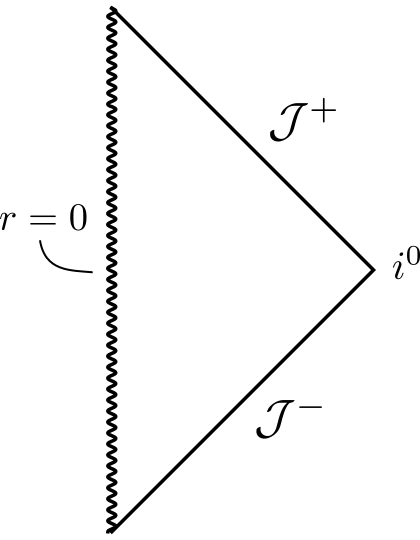
\includegraphics[width=0.35\textwidth]{cpnaked}
\caption{\textbf{Left:} The conformal compactifiction of de Sitter space viewed as a finite slab of the Einstein static universe. \textbf{Right:} The Penrose diagram for the negative mass black hole. The singularity at $r=0$ can be seen from $\scri^+$.}
\label{fig:esuds}
\end{center}
\end{figure}

\subsubsection{Example 6: Schwarzschild in $3+1$ dimensions with $M<0$}

In the Schwarzschild metric~\eqref{eq:schwarzschild}
$$
ds^2=-\left(1-\frac{2M}{r}\right)dt^2+\left(1-\frac{2M}{r}\right)^{-1}dr^2+r^2d\Omega_2^2
$$
there is no a priori restriction on the values of $M$. Let's consider the case where $M<0$ (without going into the question what ``negative mass'' really means). The term $\sfac=(1+\frac{2|M|}{r})$ is then always positive and there are no singularities in the metric except the curvature singularity at $r=0$.\\

We can construct the Penrose diagram in the same manner as in the positive mass case, by writing the metric in terms of $u=t-r_*$ and $v=t+r_*$ coordinates (with the restriction $r\geq0\iff v\geq u$) and proceeding with the conformal compactification as usual. The Penrose diagram is shown in Figure~\ref{fig:esuds}.\\

Notice that this singularity is different from the black hole singularity: it can be seen from $\scri^+$. Conversely, the singularity inside the black hole is hidden behind the horizon $r=2M$. A singularity that can be seen from $\scri^+$ is known as a \emph{naked singularity}. The white hole has a naked singularity too, as it can be seen in Figure~\ref{fig:cpkruskal}. While naked singularities occur quite frequently in solutions to Einsteins equations, their physical status is debated. Roger Penrose has formulated the \emph{cosmic censorship hypothesis: ``Nature abhors a naked singularity"}, which encapsulates the expectation that naked singularities (except for the Big Bang) are unphysical and do not occur in the real world. 
%The reason for the asymmetry between hidden and naked singularities is that the initial conditions required for the formation of a white hole are extremely special. Conversely, the initial conditions for a black hole are not special at all: indeed, the formation of black holes in a universe with matter in it is a very typical occurrence. The expectation that no


%%%%%%%%%%%%%%%%%%%%%%%%%%%%%%%%%%%%%%%%%%
%%%%%%					NEW SECTION			          	 %%%%%%
%%%%%%%%%%%%%%%%%%%%%%%%%%%%%%%%%%%%%%%%%%

\section{Charged \& Rotating Black Holes}

The Schwarzschild black hole is only the simplest among a number of black hole solutions to the Einstein equations. In fact, the astrophysical black holes for which we have observational evidence all appear to be rotating, while the Schwarzschild solution has zero angular momentum. In this section we review two further, more general, black hole solutions.

\subsection{The Reissner-Nordstr\"om Solution}
Gravity coupled to the electromagnetic field is described by the Einstein-Maxwell action
\be
S=\frac1{16\pi G}\int\sqrt{-g}\left(R-F_{\mu\nu}F^{\mu\nu}\right)d^4x\label{eq:EMaction}
\ee
where $F_{\mu\nu}=\nabla_\mu A_\nu-\nabla_\nu A_\mu$ and $A_\mu$ is the electromagnetic (four-)potential. The normalisation of the Maxwell term in~\eqref{eq:EMaction} is such that the Coulomb force between two charges $Q_1$ and $Q_2$ separated by a (large enough) distance $r$ is $G|Q_1Q_2|/r^2$. This corresponds to \emph{geometrised units of charge}.\\

The equations of motion derived from the variation of the Einstein-Maxwell action are
\be
\bal
R\munu-\frac12Rg\munu&=2\left(F_{\mu\lambda}F^\lambda_{\;\;\nu}-\frac14g\munu F_{\rho\sigma}F^{\rho\sigma}\right)\\
\nabla_\mu F^{\mu\nu}&=0.
\eal
\ee
They admit the spherically symmetric solution
\be
ds^2=-\left(1-\frac{2M}r+\frac{Q^2}{r^2}\right)dt^2+\left(1-\frac{2M}r+\frac{Q^2}{r^2}\right)^{-1}dr^2+r^2d\Omega_2^2,\label{eq:rn}
\ee
which is known as the \emph{Reissner-Nordstr\"om solution}.  The electric potential is $A_0=\frac{Q}{r}$ and the other components of $A_\mu$ vanish. We therefore interpret $Q$ as the charge of the black hole (by analogy with the electric potential of a point charge) and $M$ as its mass. Without loss of generality we will assume that $Q>0$. By a theorem analogous to Birkhoff's theorem, the Reissner-Nordstr\"om solution is the \emph{unique} spherically symmetric solution to the Einstein-Maxwell equations.\\

It is convenient to introduce the function
\be
\Delta=Q^2-2Mr+r^2=(r-r_+)(r-r_-)
\ee
where $r_\pm=M\pm\sqrt{M^2-Q^2}$. The metric then reads
\be
ds^2=-\frac{\Delta}{r^2}dt^2+\frac{r^2}{\Delta}dr^2+r^2d\Omega_2^2.
\ee
There are three separate cases to look at: $Q>M$, $Q<M$ and $Q=M$. Let's consider them in turn.
%\be
%\bal
%&\mathbf{1.}& &\text{Super-Extremal:}&\quad&Q>M\implies\Delta \mathrm{\;has\;no\;real\;roots}\\
%&(ii)& &\text{Sub-Extremal:}&\quad&Q<M\implies\Delta \mathrm{\;has\;two\;real\;roots.}\\
%&(iii)& &\text{Extremal:}&\quad&Q=M\implies\Delta \mathrm{\;has%\;one\;real\;root}\nn
%\eal
%\ee



\subsubsection{Super-Extremal RN: $Q>M$}

If $Q>M$ then $\Delta $ has no real roots and the metric is regular for all $r>0$. There is a curvature singularity at $r=0$. This is the same situation as for the negative mass black hole, and the Penrose diagram looks exactly the same (Figure~\ref{fig:esuds}).\\

%The cosmic censorship hypothesis would tell us that the super-extremal Reissner-Nordstr\"om solution is unphysical. If we started with a matter distribution such that $Q>M$, no black hole would form. [[MB1: Check books]]\\

Note that an electron has charge $e=1.6\times10^{-19}\,\mathrm{C}$ and mass $m_e=9.1\times10^{-31}\,\mathrm{kg}$. In geometrised units this means $Q=e/\sqrt{4\pi\epsilon_0G}=1.4\times10^{-29}\,\mathrm{kg}$, so $Q\gg M$. Could it be that an electron is just a charged black hole? No. The electron is a quantum mechanical object, whose Compton wavelength $\lambda=h/mc=2.4\times10^{-12}\,\mathrm{m}$ is much larger than its Schwarzschild radius $r_s=2Gm_e/c^2=1.4\times10^{-57}\mathrm{m}$.\\
 
\subsubsection{Sub-Extremal RN: $Q<M$}\label{sec:subrn}

Now $\Delta $ has two real roots $r_+>r_-$ and there are two coordinate singularities. As always, we can remove them if we find a  suitable coordinate system. Recalling our strategy with the Schwarzschild metric, let us define a tortoise coordinate $r_*$via
\be
\frac{\Delta }{r^2}dr_*^2=\frac{r^2}{\Delta }dr^2,\label{eq:rntortoiseeq}
\ee
in terms of which the metric takes the form
\be
ds^2=-\frac{\Delta }{r^2}(dt^2-dr_*^2)+r^2d\Omega_2^2.
\ee
Radial null geodesics are then given by the simple equation $t\pm r_*=const.$ (and $\theta=\phi=const.$). A solution of~\eqref{eq:rntortoiseeq} with a convenient choice of sign and integration constant is
\be
r_*=r+\frac1{2\kappa_+}\ln\left(\frac{r-r_+}{r}\right)+\frac1{2\kappa_-}\ln\left(\frac{r-r_-}{r}\right),
\ee
where
\be
\kappa_+=\frac{r_+-r_-}{2r_+^2}>0 \mand \kappa_-=\frac{r_--r_+}{2r_-^2}<0.
\ee
Define the null coordinates $u=t-r_*$ and $v=t+r_*$ and ingoing Eddington-Finkelstein coordinates $(v,r,\theta,\phi)$. In terms of the latter, the metric becomes 
\be
ds^2=-\frac{\Delta }{r^2}dr^2+drdv+r^2d\Omega_2^2,
\ee
which is regular for all $r>0$, including $r=r_+$ and $r=r_-$. To understand the spacetime structure close to $r=r_\pm$ we can use two different sets of Kruskal-type coordinates at each of the two radii:
\be
U^\pm=-\exp\left(-{\kappa_\pm}u\right) \mand V^\pm=\exp\left(\kappa_\pm u\right).
\ee
This gives rise to the Penrose diagram shown in Figure~\ref{fig:cprnsub}. Notice that a timelike trajectory can avoid $r=0$, since the $r=0$ singularity is timelike itself. In fact, to hit $r=0$, one must accelerate toward it (this time it \emph{is} like a position in space).\\

\begin{figure}[t]
\begin{center}
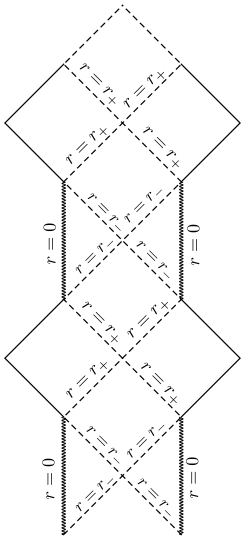
\includegraphics[width=0.35\textwidth]{cprnsub}
\caption{The Penrose diagram for the sub-extremal Reissner-Nordstr\"om solution.}
\label{fig:cprnsub}
\end{center}
\end{figure}

\subsubsection{Extremal RN: $Q=M$}
The metric of the extremal Reissner-Nordstr\"om solution is
\be
ds^2=-\left(1-\frac{M}r\right)^2dt^2+\left(1-\frac{M}r\right)^{-2}dr^2+r^2d\Omega_2^2,
\ee
which has one coordinate singularity at $r=r_+=r_-=M$. To get rid of it, define the tortoise coordinate $dr_*=(1-\frac{M}r)^{-2}dr$ such that
\be
ds^2=-\left(1-\frac{M}r\right)^2(dt^2-dr_*^2)+r^2d\Omega_2^2,\label{eq:extremalrn}
\ee
and change to ingoing Eddington-Finkelstein coordinates $(v,r,\theta,\phi)$, where $v=t+r_*$ labels ingoing null geodesics, which should be clear from a look at~\eqref{eq:extremalrn}. This leaves us with the improved line-element
\be
ds^2=-\left(1-\frac{M}r\right)dv^2+2dvdr+r^2d\Omega_2^2
\ee
which is regular at $r=M$. The inner and outer horizons have now coalesced. The result is the Penrose diagram shown in figure \textsf{(to come)}.

\subsection{Rotating Black Holes}
So far we have only discussed solutions with spherical symmetry. We now introduce the \emph{Kerr-Newman solution} (1965) to the Einstein-Maxwell equations, which describes a rotating charged black hole of mass $M$, charge $Q$ and angular momentum $J\equiv Ma$ (so $a$ is the angular momentum per unit mass). In Boyer-Lindquist coordinates $(t,r,\theta,\phi)$, in which the black hole rotates about the polar axis, the metric part of the solution is given by
\be
\bal
\!\!ds^2=
&-\left(\frac{\Delta -a^2\sin^2\theta}{\Sigma }\right)dt^2+\frac{\Sigma }{\Delta }dr^2-2\frac{a\sin^2\theta}{\Sigma }\left(r^2+a^2-\Delta \right)dtd\phi\\
&+\Sigma d\theta^2+\left(\frac{(r^2+a^2)^2-\Delta a^2\sin^2\theta}{\Sigma }\right)\sin^2\theta d\phi^2\label{eq:kn}
\eal
\ee
where where $\Sigma=r^2+a^2\cos^2\theta$ and $\Delta =r^2-2Mr+Q^2+a^2$. The components of the electromagnetic potential are
\be
A_t=\frac{Q r}{\Sigma },\qquad A_\phi=-\frac{Qar\sin\theta}{\Sigma },\qquad A_r=A_\theta=0.
\ee
%MB1: Figure here.

For $a=Q=0$, we recover the Schwarzschild solution~\eqref{eq:schwarzschild}. For $a=0$, we recover the Reissner-Nordstr\"om solution~\eqref{eq:rn}. Finally, the solution is symmetric under the simultaneous replacements $\phi\rightarrow-\phi$ and $a\rightarrow-a$, so we can set $a\geq0$ without loss of generality.\\

When a black hole is rotating, there is no analogue of Birkhoff's theorem. This means that, during gravitational collapse with rotating matter, we cannot use the same reasoning as in the spherically symmetric case to argue that, on the surface of the collapsing matter, the metric should be of the form given above. All we can say is that, after enough time has passed and matter and spacetime have ``settled down'' to equilibrium, they will be described by the Kerr-Newman solution.\\

We will investigate the structure of the simple but illustrative special case of a rotating black hole with zero charge $Q=0$. The metric~\eqref{eq:kn} then reduces to the \emph{Kerr solution} (1963):
\be
ds^2=\Sigma \left(\frac{dr^2}{\Delta }+d\theta^2\right)+(r^2+a^2)\sin^2\theta d\phi^2+\frac{2Mr}{\Sigma }\left(a\sin^2\theta d\phi-dt\right)^2-dt^2\label{eq:kerr}
\ee
where $\Delta =r^2-2Mr+a^2$ and $\Sigma =r^2+a^2\cos^2\theta$. This metric is a solution to the vacuum Einstein equations. It has coordinate singularities at 
\be
\Delta =0\iff r=r_\pm=M\pm\sqrt{M^2-a^2}. 
\ee
Below we will show a coordinate transformation that removes them. It also has a curvature singularity at 
\be
\Sigma =0\iff r=0 \;\;\text{and}\;\; \cos\theta=0.
\ee 
The latter condition implies that the curvature singularity is only there when $\theta=\frac\pi2$, i.e. when $r=0$ is approached along the equator. When approached from any other angle, there is no singularity at $r=0$.\\

There are again three cases to consider: $M<a$, $M=a$ and $M>a$. We will concentrate on the $M>a$ solution, for which there are two coordinate singularities at $r_+$ (the ``outer'' horizon) and $r_-<r_+$ (the ``inner'' horizon). To remove them, we do a coordinate transformation to ingoing Kerr coordinates $(v,r,\theta,\chi)$, where $v=t+r_*$ and $r_*$ and $\chi$ are defined by
%\footnote{The integration constants are set to such values that the ranges of $r_*$}
\be
dr_*=\frac{r^2+a^2}{\Delta}dr \mand d\chi=d\phi+\frac{a}{\Delta}dr.\label{eq:ikc}
\ee
The definition of $\chi$ implies that $\phi=const.$ does not correspond to $\chi=const.$ For example, in order to stay at $\chi=const.$ as you fall in ($dr<0$), you need to rotate too: $d\phi=-a/\Delta dr$. In terms of ingoing Kerr coordinates the metric becomes
\be
\bal
ds^2=
&-\left(\frac{\Delta-a^2\sin^2\theta}{\Sigma}\right)dv^2+2dvdr-2\frac{a\sin^2\theta}{\Sigma}(r^2+a^2-\Delta)dvd\chi\\
&-2a\sin^2\theta d\chi dr+\left[\frac{\left(r^2+a^2\right)^2-\Delta a^2\sin^2\theta}{\Sigma}\right]\sin^2\theta d\chi^2+\Sigma d\theta^2.
\eal
\ee
There are no more factors of $\Delta$ in the numerators and the metric is regular at $r_+$ and $r_-$. The only remaining singularity is the curvature singularity at $\Sigma=0$.\\

To draw the Penrose diagram is more difficult because the metric is not spherically symmetric. Since the curvature singularity at $r=0$ only appears when $\theta=\frac\pi2$, the Penrose diagram should look very different for $\theta\neq\frac\pi2$ and $\theta=\frac\pi2$. In order to represent both cases, it is customary to draw a Penrose diagram that is an amalgam of the Penrose diagram for an observer falling in from the north pole ($\theta=0$) and of that for an observer falling in in the equatorial plane ($\theta=\frac\pi2$) at fixed $\chi$. Notice that $\chi=const.$ means that $\phi$ is not constant, so the observer falling in at $\theta=\frac\pi2$ rotates about the polar axis.\\

The procedure is very similar to that for the sub-extremal Reissner-Nordstr\"om solution in section~\ref{sec:subrn}. First, perform a coordinate transformation to coordinates $(u,v,\theta,\phi)$ where $u=t+r_*$ and $v=t-r_*$ with $r_*$ as defined in~\eqref{eq:ikc}. Then, define Kruskal-type coordinates $U^\pm$ and $V^\pm$ close to $r=r_\pm$, respectively, and draw the Penrose diagram. This leads to the infinitely sequence of spacetime regions we saw in Figure~\ref{fig:cprnsub}. Up to this point, the analysis is identical for $\theta=0$ and $\theta=\frac\pi2$. The only difference is that the Penrose diagram for $\theta=0$ has a curvature singularity at $r=0$, whereas the Penrose diagram for $\theta=\frac\pi2$ has none. In the amalgam Penrose diagram for the Kerr spacetime, we indicate this by drawing an interrupted wavy line at $r=0$. The result is shown in Figure~\ref{fig:cpsubkerr}.\\

\begin{figure}[t]
\begin{center}
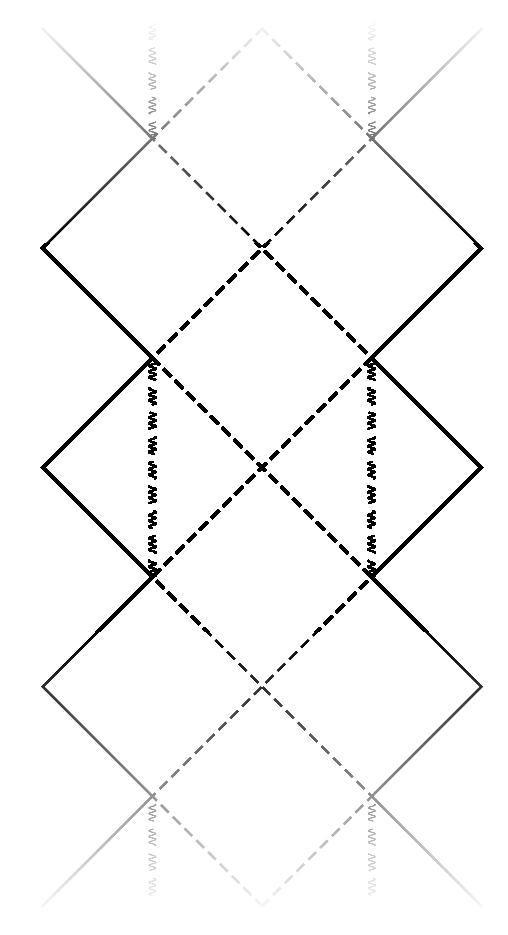
\includegraphics[width=0.35\textwidth]{cpsubkerr}
\caption{The Penrose diagram for the sub-extremal Kerr black hole.}
\label{fig:cpsubkerr}
\end{center}
\end{figure}

\subsubsection{Ring singularities}
How can it be that there is a singularity for $\theta=\frac\pi2$ but not otherwise? The simple explanation is that the singularity has the shape (topology) of a ring. Indeed, for fixed $r$, $v$ and $\theta$, the metric~\eqref{eq:kerr} becomes
\be
ds^2=\frac{(r^2+a^2)^2-\sin^2\theta(r^2-2Mr+a^2)a^2}{a^2\cos^2\theta}\sin^2\theta d\chi^2,
\ee
which tends to $ds^2=a^2\sin^2\theta d\chi^2$ as $r\rightarrow0$. When $\theta=\frac\pi2$, we obtain
\be
ds^2=a^2d\chi^2,
\ee
the metric of a ring with radius $a$. If you travel toward $r=0$ from any other angle than $\theta=\frac\pi2$, you will not encounter the singularity.  Instead, you will fall through the interior of the ``ring'' and emerge in a \emph{new} region of spacetime. 
%MB1: interesting topology. AUDIO.

\subsubsection{Closed Timelike Curves}
A \emph{closed timelike curve (CTC)}, also called a time machine, is a curve that is everywhere timelike and that eventually returns to where it started from \emph{in spacetime}. $CTC$s have been extensively explored in the context of general relativity. In fact, they are ubiquitous and appear in a number of spacetimes that are solutions to the Einstein equations.\\

Kerr spacetime is one such example: region $X$ in Figure~\ref{fig:cpsubkerr} contains  CTCs. To see this, consider a curve in region $X$ at fixed $t$, $\theta=\frac\pi2$ and $r<0$. Then
\be
ds^2=\left(r^2+a^2+\frac{2Ma}{r}\right)d\chi^2.\label{eq:kerrctc}
\ee
Close enough to the singularity, where $r$ is small and negative, $r<0$ and \linebreak $|r|<2Ma/(r^2+a^2)$,~\eqref{eq:kerrctc} is negative and the curve is timelike. Since $\chi$ is a periodic coordinate with $\chi\equiv\chi+2\pi$, the curve is also closed: it is a $CTC$.\\

However, it turns out that region $X$ is unphysical. Much like in the case of the sub-extremal RN solution of section~\ref{sec:subrn}, the inner horizon at $r=r_-$ becomes a curvature singularity in the presence of  the smallest perturbations to the Kerr metric: at the inner horizon, perturbations are infinitely blueshifted, which leads to divergences in the curvature scalars.\\



%%%%%%%%%%%%%%%%%%%%%%%%%%%%%%%%%%%%%%%%%%
%%%%%%					NEW SECTION			          	 %%%%%%
%%%%%%%%%%%%%%%%%%%%%%%%%%%%%%%%%%%%%%%%%%

\section{Killing Vectors \& Killing Horizons}

So far we have produced a number of different black hole solutions and looked at some of their features. In this section we introduce the concepts and machinery that we will need to really understand the structure of black hole spacetimes.\\%Some concepts of differential geometry (push-forwards, pull-backs, Lie derivatives etc.) will be defined without giving too much

\noindent\textsl{Notation: to denote partial derivatives we use shorthand notations such as $\partial_t=\frac{\partial}{\partial t}$ and $\partial_\mu=\frac{\partial}{\partial x^\mu}$ as well as $X{}_{\!,\mu}=\partial_\mu X$ when applied to a tensor $X$.}

\subsection{Symmetries \& Killing Vectors}

Let $(M,g)$ be a Lorentzian manifold. Given a smooth vector field $\xi$ on $M$, an \emph{integral curve} of $\xi$ is a curve $\gamma:\mathbb R\rightarrow M$ whose tangent vector is equal to $\xi$ at every point $p\in\gamma$. This can be expressed as the demand that
\be
\xi_p(f)=\left.\frac{d}{d\lambda}(f\circ\gamma(\lambda))\right|_p
\ee
for all smooth functions $f:M\rightarrow\mathbb R$. Equivalently, given a coordinate system $x^\mu$ on $M$, the components of $\xi$ in that coordinate system must satisfy
\be
\xi_p^\mu=\left.\frac{d}{d\lambda}x^\mu(\gamma(\lambda))\right|_{p},
\ee
where $\lambda$ parametrises $\gamma$.\\

When $\xi$ is smooth and everywhere non-zero, the set of integral curves form a \emph{congruence}: every point $p\in M$ lies on a unique integral curve. Given any congruence there is an associated one-parameter family of diffeomorphisms from $M$ onto itself, defined as follows: for each $s\in\mathbb R$, define $h_s:M\rightarrow M$, where $h_s(p)$ is the point parameter distance $s$ from $p$ along $\xi$, i.e. if $p=\gamma(\lambda_0)$ then $h_s(p)=\gamma(\lambda_0+s)$. These transformations form an abelian group: the composition law is $h_s\circ h_t=h_{s+t}$, the identity is $h_0$ and the inverse is $(h_s)^{-1}=h_{-s}$.\\

This leads to the concept of the \emph{Lie derivative} $\mathcal L_\xi$ along the vector field $\xi$. When applied to a vector $V$ at point $p$ it is defined as
\be
(\mathcal L_\xi V)_p=\lim_{\delta\lambda\rightarrow0}\frac{V_p-(h_{\delta\lambda})_*V_{h_{-\delta\lambda}(p)}}{\delta\lambda}.\label{eq:lie}
\ee
Here $(h_s)_*$ denotes the \emph{push-forward} associated with the group element $h_s$, which maps a vector defined at $p$ to a vector defined at $h_s(p)$. It can be shown \exercise that the Lie derivative of a vector is equal to the bracket $$(\mathcal L_\xi V)_p=\left[\xi,V\right]_p$$ where $\left[X,Y\right]^\mu=X^\nu Y^\mu_{,\nu}-Y^\nu X^\mu_{,\nu}$.\\
%[[MB1: Note that the metric $g$ has not been used anywhere so far. Lie brackets exist independently of the metric. etc.]]

The Lie derivative can be applied to any tensor on $M$, with appropriate definitions analogous to~\eqref{eq:lie}. In particular, given a metric tensor $g$ on $M$, we can take its Lie derivative. Since the components of $g$ transform covariantly (whereas vector fields transform contravariantly), the Lie derivative of $g$ involves the \emph{pull-back} $h_s^*$, which maps a covector at $h_s(p)$ to a covector at $p$:
\be
\left(\mathcal L_\xi g\right)_p=\lim_{\delta\lambda\rightarrow0}\frac{g_p-(h_{\delta\lambda})^*g_{h_{\delta\lambda}(p)}}{\delta\lambda}.
\ee
It can then be shown that
\be
(\mathcal L_\xi g)\munu=\nabla_\mu\xi_\nu+\nabla_\nu\xi_\mu.
\ee
If the metric does not change under the transformation $h_s$ we say that the transformation is an \emph{isometry} and that the metric has a \emph{symmetry}. In this case $\mathcal L_\xi g=0$, which implies
\be
\nabla_\mu\xi_\nu+\nabla_\nu\xi_\mu=0.\label{eq:killing}
\ee
This is known as \emph{Killing's equation} and a vector $\xi$ that satisfies~\eqref{eq:killing} is a \emph{Killing vector}. Note that this equation implicitly involves the metric, which is hidden in $\nabla$. Finding the symmetries of a spacetime amounts to finding the vectors that satisfy the Killing equation; this can be done either by inspection or by integrating~\eqref{eq:killing}.\\

A useful fact to know when looking for Killing vectors is the following. Given any vector field $\xi$ we can (locally) find a coordinate system $(x^1,x^2,x^3,x^4)$ in which $\xi$ takes the form
\be\xi=\frac{\partial}{\partial x^1},\ee
i.e. $\xi^\mu=(1,0,0,0)$. This implies that
\be
(\mathcal L_\xi g)\munu=\frac{\partial g\munu}{\partial x^1}.
\ee
Hence, if we find a coordinate system in which $g\munu$ is independent of one of the coordinates, say $y$, then we know that $\frac{\partial}{\partial y}$ must be a Killing vector since 
\be(\mathcal L_{\frac{\partial}{\partial y}}g)\munu=\frac{\partial g\munu}{\partial y}=0.\ee 
The converse statement is not true: if $g\munu$ depends on all the coordinates, that does not mean that that $g$ has no Killing vectors.\\

\subsubsection{Example 1: Schwarzschild}
Using the fact above, a quick look at the Schwarzschild metric
$$
ds^2=-\left(1-\frac{2M}{r}\right)dt^2+\left(1-\frac{2M}{r}\right)^{-1}dr^2+r^2d\Omega_2^2$$
reveals the two Killing vectors $k=\partial_t$ and $m=\partial_\phi$. This means that Schwarzschild spacetime is \emph{static} and \emph{axisymmetric}:

\begin{definition}
An asymptotically flat spacetime is \emph{stationary} if it admits a Killing vector $k$ such that $k^2\rightarrow-1$ asymptotically. If in addition the metric is invariant under $t\leftrightarrow -t$, the spacetime is \emph{static}.
\end{definition}

\begin{definition}
An asymptotically flat spacetime is \emph{axisymmetric} if it admits a Killing vector $\ell$ that is spacelike asymptotically and whose integral curves are closed.
\end{definition}

Schwarzschild spacetime is not just axisymmetric but spherically symmetric: it has two more spacelike Killing vectors, which together with $\partial_\phi$ generate the symmetries of a sphere --- the $SO(3)$ transformations. The other two Killing vectors cannot be ``read off'' from the metric but they can be found by solving Killing's equation.\\%MB1: show those vectors?\\

\subsubsection{Example 2: Kerr-Newman}\label{sec:knkilling}

The Kerr-Newman solution~\eqref{eq:kn} 
\be
\bal
\!\!ds^2=
&-\left(\frac{\Delta -a^2\sin^2\theta}{\Sigma }\right)dt^2+\frac{\Sigma }{\Delta }dr^2-2\frac{a\sin^2\theta}{\Sigma }\left(r^2+a^2-\Delta \right)dtd\phi\\
&+\Sigma d\theta^2+\left(\frac{(r^2+a^2)^2-\Delta a^2\sin^2\theta}{\Sigma }\right)\sin^2\theta d\phi^2\nonumber
\eal
\ee
is axisymmetric and stationary: since $g\munu$ is independent of $t$ and $\phi$, it has Killing vectors $k=\partial_t$ and $\ell=\partial_\phi$. However, the metric is not invariant under $t\leftrightarrow-t$ due to the $dtd\phi$ term, so it is not static.\\

A number of \emph{uniqueness theorems}, proved between 1967 and 1975, have established the remarkable fact that the two-parameter Kerr family (parameters $M$ and $J$) is the unique stationary asymptotically flat solution of the vacuum Einstein equations and that the three-parameter Kerr-Newman family (parameters $M$, $J$ and $Q$) is the unique stationary asymptotically flat black hole solution of the electrovacuum Einstein-Maxwell equations.

\subsection{Conservation Laws}\label{sec:conservationlaws}

In classical physics, the presence of symmetries is very closely tied to the existence of conservation laws. As we shall see in this section, this is also the case in general relativity. We first take a look at the geodesic motion of test particles.\\

Consider the action of a particle in a spacetime $(M,g)$ moving on a curve $\gamma$ with parameter $\lambda$ and endpoints $A$ and $B$. Pick a coordinate system $x^\mu$ and denote the coordinates of the curve by $x^\mu(\lambda)$. Then the action for $\gamma$ is given by
\be
I\left(x^\mu\right)=m\int d\tau=m\int_{\lambda_A}^{\lambda_B}\sqrt{-g\munu\frac{dx^\mu}{d\lambda}\frac{dx^\nu}{d\lambda}}.\label{eq:action2}
\ee
If we deform the curve by a small amount $\delta x^\mu(\lambda)$ and require the action to be stationary with respect to this variation, we obtain the Euler-Lagrange equations:
\be
\frac{\delta I}{\delta x^\mu}=0 \implies \nabla_{(\lambda)} \dot x^\mu\equiv\frac{d}{d\lambda}\dot x^\mu+\Gamma^\mu_{\rho\sigma}\dot x^\rho \dot x^\sigma \propto\dot x^\mu.\label{eq:geoeq1}
\ee
The dot denotes differentiation with respect to $\lambda$. The solutions to~\eqref{eq:geoeq1} are the \emph{geodesics} in $(M,g)$.  If the right hand side vanishes, $\nabla_{(\lambda)}\dot x^\mu=0$, the geodesic is said to be \emph{affinely parametrised} and $\lambda$ is an \emph{affine parameter}. If we set $\lambda=\tau$ then~\eqref{eq:geoeq1} reduces to
\be
\frac{d^2x^\mu}{d\tau^2}+\Gamma^\mu_{\rho\sigma}\frac{dx^\rho}{d\tau}  \frac{d x^\sigma}{d\tau} =0.
\ee
For the purpose of finding geodesics we can cast~\eqref{eq:action2} into a more useful form by introducing an independent function $e(\lambda)$ (called the \emph{auxiliary field} or \emph{einbein}):
\be
I\left(x^\mu,e\right)=\frac12\int_{\lambda_A}^{\lambda_B}d\lambda\left[e^{-1}(\lambda)g\munu \dot x^\mu\dot x^\nu-m^2e(\lambda) \right].
\ee
To see that this is equivalent to~\eqref{eq:action2}, notice that from $\delta I/\delta e=0$ we get
\be
-e^{-2}g\munu\dot x^\mu\dot x^\nu-m^2=0\implies e=\frac1m\sqrt{-g\munu\dot x^\mu \dot x^\nu}=\frac1m\frac{d\tau}{d\lambda}\label{eq:einbein}
\ee
and from $\delta I/\delta x^\mu$ we get
\be
\frac{d}{d\lambda}\dot x^\mu+\Gamma^\mu_{\rho\sigma}\dot x^\rho\dot x^\sigma=(e^{-1}\dot e)\dot x^\mu.
\ee
This equation is already the geodesic equation $\nabla_{(\lambda)}\dot x^\mu=(e^{-1}\dot e)\dot x^\mu$ and~\eqref{eq:einbein} relates $e$ to the choice of parameter $\lambda$. To turn this into the equation for an affinely parametrised geodesic, we need to set $\dot e=0$. Then $d\tau/d\lambda=const.$, which implies that $\lambda=a\tau+b$.\\

%We can now discuss the connection between Killing vectors and conserved quantities for geodesics. 
Consider now an infinitesimal translation of the curve $\gamma$ along a Killing vector field $k$ (leaving $e$ unchanged). In the coordinate chart $x^\mu$ this corresponds to
\be
x^\mu\rightarrow x^\mu+\alpha k^\mu
\ee
where $\alpha$ is an infinitesimal constant. Then the action will be changed by an amount
\be
\bal
\delta I
&=I(x^\mu+\alpha k^\mu,e)-I(x^\mu,e)\\
&=\frac\alpha2\int d\lambda\left[e^{-1}\left( g\munu \dot k^\mu\dot x^\nu+g\munu \dot x^\mu\dot k^\nu+g_{\mu\nu,\sigma} \dot x^\mu\dot x^\nu k^\sigma\right)\right]\\
&=\frac\alpha2\int d\lambda\left[e^{-1}\left( g\munu \dot x^\sigma \dot x^\nu k^\mu{}_{\!,\sigma}+g\munu \dot x^\mu\dot x^\sigma k^\nu{}_{\!,\sigma}+g_{\mu\nu,\sigma} \dot x^\mu\dot x^\nu k^\sigma\right)\right]\\
&=\frac\alpha2\int d\lambda\left[e^{-1}\dot x^\mu\dot x^\nu \left( g_{\sigma\nu}k^\sigma{}_{\!,\mu}+g_{\mu\sigma} k^\sigma{}_{\!,\nu}+g_{\mu\nu,\sigma}  k^\sigma\right)\right]\\
&=\frac\alpha2\int d\lambda\left[e^{-1}\dot x^\mu\dot x^\nu \left(\nabla_\mu k_\nu+\nabla_\nu k_\mu\right)\right]\\
&=0
\eal
\ee
where the last line follows from the fact that $k$ satisfies Killing's equation. To get from the second to the third line we used the fact that $\dot k^\mu=\frac{d}{d\tau} k^\mu=\frac{d x^\nu}{d\tau}\partial_\nu k^\mu=\dot x^\nu k^\mu{}_{\!,\nu}.$ We see that $k$ being Killing leads to a symmetry of the particle action. Associated with this symmetry is a quantity (charge) that is conserved along geodesics:\\

\noindent\textbf{Claim.} Let $k$ be a Killing vector. Then
\be
Q= k^\mu p_\mu
\ee
is conserved along geodesics, where $p_\mu$ is the momentum of the particle defined by
\be
p_\mu=\frac{\partial\mathcal L}{\partial\dot x^\mu}=e^{-1} g\munu \dot x^\nu=mg\munu\frac{dx^\nu}{d\tau}.
\ee
The last equality follows from equation~\eqref{eq:einbein} for $e$.\\

\noindent\textbf{Proof.} Consider a small variation $\delta x^\mu=\alpha k^\mu$ generated by the Killing vector $k$. Set $\lambda=\tau$ for simplicity (the proof for general $\lambda$ is similar). As shown above, such variations leave the action invariant: $\delta I=0$. Defining the Lagrangian density $\mathcal L$ as $I=\int \mathcal L d\lambda$, we then have
\be
\frac{\partial\mathcal L}{\partial x^\mu}\delta x^\mu+\frac{\partial\mathcal L}{\partial\dot x^\mu}\delta \dot x^\mu=0.
\ee
Using the Euler-Lagrange equations
\be
\frac{\partial\mathcal L}{\partial x^\mu}=\frac{d}{d\tau}\frac{\partial\mathcal L}{\partial \dot x^\mu}=\dot p_\mu,
\ee
the previous equation can be written as
\be
0=\dot p_\mu \alpha k^\mu+p_\mu\alpha\dot k^\mu=\alpha\frac{d}{d\tau}(k^\mu p_\mu)=\alpha\frac{d}{d\tau}Q.
\ee
Therefore $Q$ is constant along geodesics.\\

\subsubsection{Example 1: Schwarzschild}
Recall the Killing vector $k=\partial_t$ in Schwarzschild spacetime. Then $k^\mu=(1,0,0,0)$ and we have
\be
Q= k^\mu p_\mu=k^\mu m g\munu \dot x^\nu=mg_{00}\dot x^0=-m\sfac \frac{dt}{d\tau}\equiv-E,
\ee
where we have identified $Q$ with minus the energy of the particle in the rest frame of the black hole. This agrees with the the definition of the constant $\epsilon=E/m$ in equation~\eqref{eq:ssenergy} of section~\ref{sec:schwarzschild}.\\

%[[MB1: AUDIO: special case etc]]

The conserved quantity associated with $\ell=\partial_\phi$ is
\be
Q=m g_{33}\dot x^3=mr^2\sin^2\theta\dot\phi\equiv J,
\ee
the angular momentum of the particle along the axis of symmetry as measured by an observer at rest at infinity.


\subsubsection{Example 2: Kerr}

The vectors $k$ and $\ell$ are also Killing vectors for the Kerr metric~(\ref{eq:kn},\ref{eq:kerr}):
\be
ds^2=\Sigma \left(\frac{dr^2}{\Delta }+d\theta^2\right)+(r^2+a^2)\sin^2\theta d\phi^2+\frac{2Mr}{\Sigma }\left(a\sin^2\theta d\phi-dt\right)^2-dt^2.\nonumber
\ee
In Schwarzschild spacetime, you (or a test particle) can travel along integral curves of $k=\partial_t$ anywhere outside the horizon --- you will then appear stationary\footnote{The word ``stationary'' here has nothing to do with the definition of a stationary spacetime. When used to describe the relative motion of one observer or test particle with respect to another observer, stationary just means ``not moving in space'' from the point of view of the latter.} to observers at infinity, since your position in space is not changing. This is possible because $g_{00}$ is negative everywhere for $r>2M$, so that $k^2=g_{00}$ is negative and the integral curves of $k$ are timelike. It turns out that this is not the case in Kerr spacetime: there is a region around the outer horizon, called the \emph{ergosphere} or \emph{ergoregion}, in which it is impossible for you (and any test particle) to remain stationary with respect to observers at infinity --- everything rotates. This happens because
\be
g_{00}=-\left(1-\frac{2Mr}{\Sigma}\right)
\ee
becomes positive in the region
\be
\frac{2Mr}{\Sigma}>1\implies \xi(r)\equiv\Sigma-2Mr=r^2+a^2\cos^2\theta-2Mr<0,
\ee
part of which lies \emph{outside} the outer horizon $r=r_+$ when $a\neq0$. This is easy to see by noting that the equation for $\xi(r)$ is a parabola with roots at $\tilde r_\pm=M\pm\sqrt{M^2-a^2\cos^2\theta}$ and $\tilde r_+$ is bigger than $r_+=M+\sqrt{M^2-a^2}$ for $\theta\neq 0,\pi$. Hence $g_{00}$ is positive in the ellipsoidal region $r_+<r<\tilde r_+$, which has a maximum extent on the equator $\theta=\frac\pi2$ where $\tilde r_+=M+\sqrt{M^2+a^2}$.\\

In the ergoregion, orbits of $\partial_t$ are not timelike, so you cannot travel along them and remain stationary with respect to observers at infinity. In order for a curve $x^\mu=(t,r,\theta,\phi)$ to be timelike, its tangent vector $u^\mu=dx^\mu/d\tau$ must satisfy $u^2=-1$. But in the ergoregion, \emph{every} term in $u^2=g\munu u^\mu u^\nu$ is positive except for $g_{t\phi} u^t u^\phi$, which means that $u^\phi=d\phi/d\tau$ must be non-zero. Moreover, since  $u^t>0$ for a future-directed worldline and $g_{t\phi}<0$, $u^\phi$ must be positive. Any timelike worldline is therefore dragged around in the direction of rotation of the black hole. This effect is an example of \emph{frame dragging}.

\subsubsection{Example 3: The Penrose Process}

The Penrose process is a process that allows you to extract energy from a rotating black hole. Imagine sending a particle into the ergoregion. Prepare it carefully such that, once in the ergoregion, it decays into two particles, one of which falls into the black hole and one of which escapes the ergoregion again. Denote the energy of the initial particle by $E=-k_\mu p^\mu$ and that of the final particles by $E_1=-k_\mu p_1^\mu$ and $E_2=-k_\mu p_2^\mu$, where $k$ is the asymptotically timelike Killing vector. Conservation of four-momentum $p^\mu=p_1^\mu+p_2^\mu$ implies that $E=E_1+E_2$. The fact that $k$ is spacelike in the ergoregion allows you to arrange the decay such that  the energy of the particle that falls into the black hole is negative with respect to you: $E_1=k_\mu p_1^\mu<0$. To see this, choose a coordinate system in which $k^\mu=(0,x,0,0)$. Prepare your decay such that $p_1^\mu=(1,y,0,0)$, where $y$ is small enough for $p_1$ to be timelike and adjusted such that $xy>0$. Then $E_1$ is negative and $E_2>E$: the particle that reemerges from the ergoregion has more energy than the particle you sent in. 
%MB1: mention limit, schwarzschild, make picture. use wald for discussion.

\subsection{Hypersurfaces}
%The horizon is a central aspect of black holes. So far we have audio.\\%MB1

Let $S(x)$ be a smooth function of the spacetime coordinates. Consider the family of hypersurfaces $S(x)=const.$ The normal vector to $S(x)=const.$ is given by
\be
n^\mu=f(x) g^{\mu\nu}\partial_\nu S,
\ee
where $f(x)$ is an arbitrary (smooth) normalisation function. A hypersurface is spacelike (timelike) when $n$ is timelike (spacelike) everywhere on it. When the hypersurface is timelike (spacelike) we can always find an $f(x)$ such that $n^2=-1$ ($n^2=+1$). A hypersurface is null when $n$ is null, $n^2=0$.\\

\subsubsection{The induced metric}\label{sec:inducedmetric}

Consider a spacelike (timelike) hypersurface $\Sigma$ in a spacetime $(M,g)$. Normalise the normal $n$ to $\Sigma$ such that $n^2=-1$ ($n^2=+1$). Then the \emph{induced metric} $h$ on $\Sigma$ is given by 
\be
h_{\mu\nu}=g_{\mu\nu}+n_\mu n_\nu.
\ee
The metric $h$ is the restriction of $g$ onto $\Sigma$: while $h$ is degenerate on the full tangent space at any point $p\in\Sigma$, it is positive definite for spacelike $\Sigma$ (Lorentzian for timelike $\Sigma$) on the subspace of the tangent space spanned by vectors tangent to curves in $\Sigma$ (i.e. vectors $v$ that satisfy $v.n=0$).\\

To give an example, consider a spatial slice $\Sigma$ defined by $S(x)=t=const.$ in $3+1$ dimensional Minkowski space with Cartesian coordinates $(t,\mathbf x)$. Then $n^\mu=(1,0,0,0)$ and \be
h_{\mu\nu}=g_{\mu\nu}+n_\mu n_\nu=\text{diag}(-1,1,1,1)+\text{diag}(1,0,0,0)=\text{diag}(0,1,1,1).
\ee
On the spatial slice $\Sigma$, $h$ is just the positive definite three-dimensional flat Euclidean metric. Next, consider a timelike hypersurface $\Sigma$ defined by $S(x)=x^1=const.$ with normal $n^\mu=(0,1,0,0)$. The induced metric on it is $h_{\mu\nu}=\mathrm{diag}(-1,0,1,1)$, which carries Lorentzian signature on the subspace of the tangent space spanned by vectors tangent to $\Sigma$.


\subsubsection{Null hypersurfaces}

For a null hypersurface $\Sigma$, the normal $n$ to $\Sigma$ is also tangent to $\Sigma$, since, by definition, a vector $t$ is tangent to $\Sigma$ if $t.n=0$. This is satisfied by $n$ itself when it is null: $n.n=0$.
When the normal is null we will henceforth use the symbol $\ell$ instead. The normal $\ell$ is tangent to curves $x^\mu(\lambda)$ in $\Sigma$: $\ell^\mu=\frac{dx^\mu}{d\lambda}$. In fact, the integral curves of $\ell$ are \emph{null geodesics}:\\
%, the surface $r=2M$ in Schwarzschild spacetime is null. MB1: finish. And Minkowski examples. The normal vectors to null hypersurfaces have a peculiar property: they are also tangent to the hypersurface. Indeed if $n^\mu=g^{\mu\nu}\partial_\nu \Sigma$ is null then?\\

\noindent\textbf{Claim:} For a null hypersurface $\Sigma$, the integral curves in $\Sigma$ of the normal $\ell$ are null geodesics.\\

\noindent\textbf{Proof:} For $\ell^\mu=f g^{\mu\nu}\partial_\nu S$ we have
\be
\bal
\ell.\nabla \ell^\nu
&=\ell^\mu\nabla_\mu(fg^{\nu\rho}\partial_\rho S)\\
&=\ell^\mu(\nabla_\mu f)g^{\nu\rho}\partial_\rho S+f\ell^\mu g^{\nu\rho}\nabla_\mu\partial_\rho S\\
&=(\ell.\nabla f)f^{-1}\ell^\nu+f\ell^\mu g^{\nu\rho}\nabla_\mu\partial_\rho S.\label{eq:proofnullgeo}
\eal
\ee
The second term reduces as follows:
\be
\bal
\ell^\mu fg^{\nu\rho}\nabla_\mu\partial_\rho S
&=f\ell^\mu g^{\nu\rho}\nabla_\rho\partial_\mu S\\
&=f\ell^\mu g^{\nu\rho}\nabla_\rho(f^{-1}\ell_\mu)\\
&=fg^{\nu\rho}(\nabla_\rho f^{-1})\ell^2+\ell^\mu g^{\nu\rho}\nabla_\rho \ell_\mu\\
&=\frac12 g^{\nu\rho}\nabla_\rho(\ell^2)\\
&\propto \ell^\nu
\eal
\ee
using the fact that $\ell^2=0$ on $\Sigma$ in the third line. In the last line, note that $\ell^2=0$ on $\Sigma$ does not necessarily imply $\nabla_\rho(\ell^2)=0$, because $\ell^2$ can be non-zero outside of $\Sigma$ and hence its derivative can be non-zero. However, any non-zero contribution to $\nabla_\rho(\ell^2)$ must be proportional to the normal to $\Sigma$: $\nabla_\rho(\ell^2)\propto\ell_\rho$. Together with~\eqref{eq:proofnullgeo} this implies that $\ell.\nabla \ell^\nu\propto \ell^\nu$ and therefore the integral curves of $\ell^\mu$ are geodesics.\qed\\
 
 If the integral curves of $\ell^\mu$ are not affinely parametrised, then we can always find some function $h(x)$ such that $\tilde \ell^\mu=h(x)\ell^\mu$  has affinely parametrised integral curves, i.e. $\tilde\ell.\nabla\tilde\ell^\mu=0$. These curves are called the \emph{null geodesic generators} of the null hypersurface.
 %MB1: example in notes.
 
 \subsection{Killing Horizons}

A null hypersurface $\Sigma$ is a \emph{Killing horizon} of a Killing vector $\xi$ if $\xi$ is normal to $\Sigma$ on $\Sigma$. Let $\ell$ be normal to $\Sigma$ and affinely parametrised such that $\ell.\nabla\ell=0$. Then, for some function $f$, $\xi=f\ell$ on $\Sigma$. It follows that $\xi$ satisfies
\be
\bal
\xi^\mu\nabla_\mu\xi^\nu&=f\ell^\mu\nabla_\mu(f\ell^\nu)\\
&=f\ell^\mu\ell^\nu\nabla_\mu f+f^2\ell^\mu \nabla_\mu\ell^\nu\\
&=f\ell^\nu \ell^\mu\nabla_\mu f\\
&\equiv \kappa\xi^\nu\label{eq:surfacegrav}
\eal
\ee
on $\Sigma$. In the last line we have defined $\kappa$, the \emph{surface gravity}: $\xi^\mu\nabla_\mu\xi^\nu=\kappa\xi^\nu$. It takes its name from the fact that $\kappa$ is constant over the horizon and equals the force that an observer at infinity would have to exert in order to keep a unit mass at the horizon.\\%MB1:mention unphysicality of this situation and include calculation from blau

\subsubsection{Example 1: Schwarzschild} 
In Schwarzschild spacetime, the surfaces of constant $r$ are the ``cylinders''of constant $S(r)=r$ and the black hole horizon corresponds to the particular surface $S(r)=2M$. To find the normal vector $\ell^\mu=f g^{\mu\nu}\partial_\nu S$ to the horizon, let us work in $IEF$ coordinates. We need the inverse of the $IEF$ metric~\eqref{eq:ef1}, which is given by
\be 
g^{\mu\nu}=
\begin{pmatrix}
0 & 1 & 0 & 0\\
1 & \sfac & 0 & 0\\
0 & 0 & 1/r^2 & 0\\
0 & 0 & 0 & 1/r^2\sin^2\theta
\end{pmatrix}.
\ee
The normal vector to the surface $S(r)=2M$ is then
\be
\textstyle \ell^\mu=f(g^{vr}\partial_r S,g^{rr}\partial_r S,0,0)=f\left(1,\sfac,0,0\right)=f(1,0,0,0)=f \partial_v.
\ee
This vector is null at $r=2M$ since $\ell^2=f^2 g^{rr}=f^2\sfac=0$ at $r=2M$. Hence $r=2M$ is a null hypersurface. $\ell=f\partial_v$ is a Killing vector (since $g\munu$ is independent of $v$) and it is timelike everywhere outside the horizon.\\

Remember that we already encountered a timelike Killing vector in Schwarzschild spacetime: $\partial_t$ in Schwarzschild coordinates. In fact $\partial_t$ and $\partial_v$ are the same vector field. To check this, denote Schwarzschild coordinates by $(t,r,\theta,\phi)$ and $IEF$ coordinates by $(v,\tilde r,\tilde\theta,\tilde \phi)$. Then
\be
\bal
dv&=dt+\textstyle\sfac^{-1}dr\\
d\tilde r&=dr\\
d\tilde\theta&=d\theta\\
d\tilde\phi&=d\phi\\
\eal
\ee
and therefore
\be
\partial_t = \frac{\partial v}{\partial t} \partial_v+\frac{\partial\tilde r}{\partial t} \partial_{\tilde r}+\frac{\partial\tilde\theta}{\partial t} \partial_{\tilde\theta}+\frac{\partial\tilde\phi}{\partial t} \partial_{\tilde \phi}=\partial_v.
\ee\\

The surface gravity $\kappa$ is evaluated most easily in $IEF$ coordinates. The equation~\eqref{eq:surfacegrav} defining $\kappa$ is a vector equation so we only need to evaluate one of its components. For $\xi=\partial_v$, the $\mu=v$ component of $\xi^\sigma\nabla_\sigma\xi^\mu$ is
\be
\xi^\sigma\nabla_\sigma\xi^v=\xi^\sigma\xi^v{}_{,\sigma}+\xi^\sigma\Gamma^v_{\sigma\rho}\xi^\rho=\Gamma^v_{vv}.\label{eq:sssg}
\ee
Now
\be
\Gamma^v_{vv}=\frac12 g^{v\sigma}\left(g_{v\sigma,v}+g_{\sigma v,v}-g_{vv,\sigma}\right)=\frac12g^{vr}(-g_{vv,r})=\frac{M}{r^2},
\ee
which, on the horizon, reduces to $\Gamma^v_{vv}=1/4M$. Substitution into~\eqref{eq:sssg} then gives $\kappa=1/4M$.\\

Note that the particular normalisation of $\xi$ is important. Had we used a vector with a different normalisation $\tilde \xi=c\xi$ we would have obtained $\tilde \xi.\nabla\tilde\xi^\nu=(c\kappa)\tilde\xi^\nu$, leading to a different value $\tilde\kappa=c\kappa$ for the surface gravity. In Schwarzschild spacetime, the normalisation that leads to $\kappa=1/4M$ is fixed by requiring that $\xi^2=-1$ asymptotically.
%MB1: exercise show RN surface gravity

\subsubsection{Example 2: Kerr}

The Killing horizon of a Kerr black hole is slightly more complicated in an interesting way. Recall the Killing vectors $k=\partial_t$ and $m=\partial_\phi$ of the Kerr-Newman black hole in Boyer-Lindquist coordinates $(t,r,\theta,\phi)$ of section~\ref{sec:knkilling}. Let's consider the zero charge case of the Kerr black hole. In Kerr coordinates $(v,r,\theta,\chi)$ --- defined above~\eqref{eq:ikc} --- the Killing vectors correspond to $k=\partial_v=\partial_t$ and $m=\partial_\chi=\partial_\phi$. The frame dragging effect translates to the fact that $k$ is \emph{not} normal to the horizon. Instead, for the rotating Kerr black hole, the normal to the horizon is a combination of $k$ and $m$ \exercise\!:
\be
\xi=k+\Omega_H m,\label{eq:defomegah}
\ee
where $\Omega_H=a/(r_+^2+a^2)$ is interpreted as the angular velocity of the black hole. The intuition here is that as you move forward in time along a null generator of the horizon, you also have to rotate by a certain amount. Given $\xi$ we can evaluate the surface gravity $\kappa_+$ on the outer horizon $r=r_+$ using $\xi.\nabla\xi^\nu=\kappa\xi^\nu$, which evaluates to \exercise
\be
\kappa_+=\frac{r_+-r_-}{2(r_+^2+a^2)}.\label{eq:rnkappa}
\ee

\subsection{Black Hole Uniqueness}
As already mentioned in section~\ref{sec:knkilling}, the Kerr-Newman three-parameter family is the unique stationary black hole solution of the Einstein-Maxwell theory. An equilibrium black hole in the presence of the electromagnetic field is therefore fully characterised by the three numbers $M$, $J$ and $Q$.\\

However, the electromagnetic field is only one among many matter fields in Nature. Through a series of theorems known as ``no hair'' theorems it has been established that, in general, black holes have no other properties besides mass, angular momentum and charge (of whichever fields are present). To illustrate the general spirit of these proofs, we look at a simple example here.\\

\noindent\textbf{Claim:} A static black hole cannot be the source of a real (minimally coupled) scalar field.\\

\noindent\textbf{Proof:} Let $\phi$ be a real scalar field that satisfies the Klein-Gordon equation
\be
\nabla^2\phi-m^2\phi=0.\label{eq:kleingordon}
\ee
By the word ``static'' in the claim we mean that scalar field and spacetime (i.e. the metric field) have settled down to equilibrium, which implies that the scalar field does not vary in time anymore: ``$\dot\phi=0$''. In covariant language the statement is that there exists a timelike Killing vector $k\;(=\partial_t)$ of the metric such that $k^\mu\nabla_\mu\phi=0$. Given $k$ we can foliate the spacetime by $t=const.$ hypersurfaces whose unit normals $n$ are proportional to $k$, $n\propto k$. The black hole horizon is a Killing horizon of $k$.\\

Consider the integral
\be
I=\int_{R} \phi(\nabla^2\phi-m^2\phi)\sqrt{-g}d^4x,
\ee
where $V\subset M$ is the spacetime region \emph{outside} of the horizon. From the Klein-Gordon equation~\eqref{eq:kleingordon} it follows immediately that $I=0$. On the other hand, using Stokes' theorem to integrate by parts the first term, we get
\be
I=\int_V (-g^{\mu\nu}\nabla_\mu\phi\nabla_\nu\phi-m^2\phi^2)\sqrt{-g}d^4x+\int_{\partial V}\phi\nabla_\mu\phi dS^\mu\label{eq:int1}
\ee
where $\partial V$ is the boundary of the region $V$ and $dS^\mu$ is the normal surface element on $\partial V$.\\

We now show that the surface integral in~\eqref{eq:int1} vanishes identically. There are four contributions to $\partial V$: the horizon $r=2M$, the surfaces $t=\pm\infty$ and the surface $r\rightarrow\infty$ (the ``sphere at infinity''). On the horizon and on the $t=\pm\infty$ surfaces, the normal surface element is proportional to $k$, so the integrand vanishes: $\nabla_\mu\phi dS^\mu\propto k^\mu\nabla_\mu\phi=0$. We are left with the boundary term at $r\rightarrow\infty$. To see that this vanishes too, note that since the spacetime is static and asymptotically flat, the metric takes the form%MB1: justify
\be
ds^2=f(r)dt^2+g(r) dr^2+r^2d\Omega_2^2
\ee
where $f(r)=-1+f_1 r^{-1}+\mathcal O(r^{-2})$ and $g(r)=1+g_1 r^{-1}+\mathcal O(r^{-2})$. Using\linebreak $\nabla^2=\frac1{\sqrt{-g}}\partial_\mu(\sqrt{-g} g^{\mu\nu}\partial_\nu)$, a quick expansion shows that the leading terms in the Klein-Gordon equation in the limit $r\rightarrow\infty$ are
\be
\partial_r^2\phi + 2 r^{-1}\partial_r\phi-m^2\phi=0,
\ee
which implies that the field must fall off like $\phi\sim1/r$ or faster. For a sphere of radius $r$ the normal surface element takes the form $dS\propto r dr\partial_r$, so the leading contribution in the integrand is $\phi \nabla_\mu\phi dS^\mu\propto r dr\phi\partial_r\phi\sim dr/r^2$. The integral of this vanishes in the limit $r\rightarrow\infty$.\\

Hence, the first integral in~\eqref{eq:int1} must vanish identically. In terms of the induced metric $h_{\mu\nu}=g_{\mu\nu}-n_\mu n_\nu$ on hypersurfaces of $t=const.$ the integrand reads
\be
g^{\mu\nu}\nabla_\mu\phi\nabla_\nu\phi=h^{\mu\nu}\nabla_\mu\phi\nabla_\nu\phi+(n.\nabla\phi)^2=h^{\mu\nu}\nabla_\mu\phi\nabla_\nu\phi\geq0
\ee
having dropped the second term due to the fact that $n\propto k$ and $k.\nabla\phi=0$. The last inequality follows from the fact that $h$ is positive definite (see section~\ref{sec:inducedmetric}). Therefore, the integrand is always negative or zero and the integral is zero only if the integrand vanishes everywhere.
For $m>0$ this implies that $\phi=0$ everywhere. For $m=0$ it implies that $\nabla_\mu\phi=0\implies\phi=const.$ everywhere, which is physically indistinguishable from $\phi=0$ everywhere.\qed
%MB1: Finish

\subsection{Komar Integrals}
%MB1: Intro
For a Killing vector $k$, the Killing equation $\nabla_\mu k_\nu+\nabla_\nu k_\mu=0$ is the statement that the symmetric part of $\nabla_\mu k_\nu$ vanishes: $\nabla_{(\mu}k_{\nu)}=0$. It follows that $\nabla_\mu k_\nu$ is antisymmetric:
\be
\nabla_\mu k_\nu =\nabla_{[\mu}k_{\nu]}=\frac12\left(\nabla_\mu k_\nu-\nabla_\nu k_\mu\right)\equiv K_{\mu\nu}.
\ee
The tensor $K_{\mu\nu}$ looks similar to the electromagnetic tensor $F_{\mu\nu}=\nabla_\mu A_\nu-\nabla_\nu A_\mu$ and, indeed, just as Maxwell's equations lead to a conserved electric charge, Einstein's equations lead to a conserved quantity when the spacetime has a Killing vector. This is expressed most conveniently in the language of differential forms.\\



\begin{center}\rule{\textwidth}{0.4pt}\end{center}
%\framebox[\textwidth][l]{\begin{minipage}[c]{0.95\textwidth}
\begin{center}\noindent\textbf{Lightening Review of Differential Forms}\end{center}
Given a $d$-dimensional spacetime $(M,g)$, a \emph{differential form} of order $k$ (or $k$-form) on $M$ is a totally antisymmetric covariant $k$-index tensor. By definition, zero-forms are functions and one-forms are covectors. Given a (local) coordinate chart $x^\mu$ on $M$, the coordinate differentials $dx^1,dx^2,\ldots,dx^d$ are examples of $1$-forms and together they form a complete basis. A general one-form can therefore be written as $F=F_\mu dx^\mu$, where $F_\mu$ are the components of $F$.  A $k$-form $F$ can be written as
\be
F=\frac1{k!}F_{\mu_1\mu_2\ldots \mu_k}\,dx^{\mu_1}\wedge dx^{\mu_2}\ldots\wedge dx^{\mu_k},
\ee
where $\wedge$ is the antisymmetric \emph{wedge product}: $dx^\alpha\wedge dx^\beta=-dx^\beta\wedge dx^\alpha$.  The \emph{exterior derivative} of a $k$-form $F$ is defined as the $(k+1)$-form $dF$ whose components are
\be
(dF)_{\mu_1\mu_2\ldots\mu_{k+1}}=(k+1)\partial_{\,[\mu_1}\omega_{\mu_2\mu_3\ldots\mu_{k+1}]}.
\ee
A consequence of the antisymmetrisation in the definition is that $d(dF)=0$ always. The Hodge star $\star$ is a linear map that sends $k$-forms to $(d-k)$-forms. If $F$ is a $k$-form, then $\star F$ is defined as the $(d-k)$-form whose components are
\be
(\star F)_{\mu_1\mu_2\ldots\mu_{d-k}}=\sqrt{-g}\,\varepsilon_{\mu_1\mu_2\ldots\mu_{d-k}}{}^{\sigma_1\sigma_2\ldots\sigma_{k}}F_{\sigma_1\sigma_2\ldots\sigma_k},
\ee
where $\varepsilon$ denotes is the \href{http://en.wikipedia.org/wiki/Levi-Civita_symbol}{Levi-Civita symbol}. Stokes' theorem states that for any form $F$ the integral of the exterior derivative $dF$ over a region $R\subseteq M$ is equal to the integral of $F$ over the boundary $\partial R$ of $R$:
\be
\int_R dF=\int_{\partial B} F.
\ee
%\end{minipage}}
\vspace{-25pt}\begin{center}\rule{\textwidth}{0.4pt}\end{center}

\vspace{25pt}

The electromagnetic tensor defines the two-form $F=\frac12 F_{\mu\nu}\,dx^\mu \wedge dx^\nu$. In terms of the four-potential $A=A_\mu dx^\mu$ it is given by $F=dA$, which implies that  \linebreak $d F=d(dA)=0$. Maxwell's equations are completely encapsulated in the two equations
\be
\bal
d\star F&=4\pi\star j\\
d\star j&=0
\eal
\ee
where $j=j_\mu dx^\mu$. The second equation is the continuity equation. The Hodge star $\star$ exchanges magnetic and electric fields, i.e. the magnetic and electric components of $F$ are interchanged in $\star F$. Consider the electric charge in some spacelike region $B$, which we define as
\be
Q(B)=\int_B\star j=\frac1{4\pi}\int_Bd\star F=\frac1{4\pi}\int_{\partial B}\star F.\label{eq:charge}
\ee
The last equality follows from Stoke's theorem. This charge is conserved, which can be shown as follows. Take any two spacelike surfaces $B_1$ and $B_2$. Consider the cylindrical region $V$, which is bounded by $B_1$ and $B_2$ and chosen to be large enough that all the sources (i.e. the support of $j$) lie inside $V$. In other words $j=0$ on the cylindrical boundaries and outside of $V$. An illustrative example is shown in Figure~\ref{fig:chargeplot}, where $V$ corresponds to the solid cylinder-like region between $B_1$ and $B_2$. By virtue of the continuity equation we have:
\be
\bal
0
&=\int_V d\star j\\
&=\int_{\partial V}\star j\\
&=\int_{B_1}\star j-\int_{B_2}\star j\\
&=\frac1{4\pi}\int_{\partial B_1}\star F-\frac1{4\pi}\int_{\partial B_2}\star F\\
&=Q(B_1)-Q(B_2),
\eal
\ee
which proves that $Q$ is conserved.\\

\begin{figure}[t!]
\begin{center}
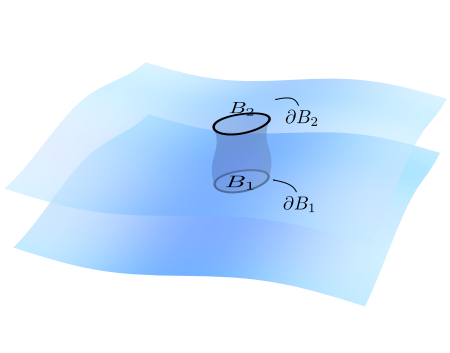
\includegraphics[width=0.75\textwidth]{chargeplot3}
\caption{Two spacelike slices with subregions $B_1$ and $B_2$. $V$ is the spacetime volume traced out between $B_1$ and $B_2$. The regions are chosen in such a way that there are no sources outside of V.}
\label{fig:chargeplot}
\end{center}
\end{figure}

Let's turn to the analogous situation for $K_{\mu\nu}$. The associated two-form is defined as $K=\frac12 K_{\mu\nu}\,dx^\mu\wedge dx^\nu$. How does $K$ show up in Einstein's equations? First note that $(\nabla_\mu\nabla_\nu-\nabla_\nu\nabla_\mu)k^\sigma=R^{\,\sigma}{}_{\!\rho\mu\nu} k^\rho$. For $\sigma=\mu$ we get $\nabla_\mu\nabla_\nu k^\mu=R_{\rho\nu} k^\rho$ or
\be
\nabla_\mu K^\mu{}_\nu= R_{\rho\nu} k^\rho,
\ee
which looks just like $\nabla_\mu F^\mu{}_\nu=4\pi j_\nu$. Einstein's equations $R_{\mu\nu}-\frac12 R g_{\mu\nu}=8\pi G T_{\mu\nu}$ can be written as
\be
R_{\rho\nu}=8\pi G\left(T_{\rho\nu}-\frac12 g_{\rho\nu} T\right).
\ee
Let 
\be
\zeta_\nu\equiv \frac1{8\pi G} R_{\rho\nu}k^\rho
\ee 
and $\zeta=\zeta_\nu dx^\nu$. Then Einstein's equations take the form
\be
\bal
d\star K&=8\pi G\star\zeta\\
d\star\zeta&=0.
\eal
\ee
In analogy to~\eqref{eq:charge} we can then define a \emph{Komar integral}
\be
Q_k(B)\equiv \frac{c}{8\pi G}\int_{\partial B}\star K
\ee
for any Killing vector $k$. It can be shown that, for $B$ large enough such that all matter is inside of it and spacetime is vacuum outside of it,  $Q_k(B)$ is conserved.\\
%MB1: Finish with audio and stuff from notes.

The physical interpretation of $Q_k$ depends on the Killing vector $k$. Some examples (whose proof is left as an~\textsf{exercise}) for appropriate choices of constants $c$ and regions $B$ are:
\begin{itemize}
\item In Schwarzschild spacetime, $Q_k(B)=M$ where $k=\partial_t$.
\item In Kerr spacetime, $Q_m(B)=J$ where $m=\partial_\phi$.
\item In Kerr-Newman spacetime, $Q_k(B)=M$ and $Q_m(B)=J$.
\end{itemize}

%For completeness, the Penrose diagrams for the remaining two cases $M^2<a^2$ and $M=a$ are shown in figure \textsf{(to come)}. The analysis is very similar to that of the extremal and super-extremal RN solutions.




%%%%%%%%%%%%%%%%%%%%%%%%%%%%%%%%%%%%%%%%%%
%%%%%%					NEW SECTION			          	 %%%%%%
%%%%%%%%%%%%%%%%%%%%%%%%%%%%%%%%%%%%%%%%%%


\section{Black Hole Thermodynamics}
%MB1: Write what Fay said in lecture before starting this.
\subsection{Overview}
In 1973, Bardeen, Carter and Hawking (BCH) wrote a paper titled ``The Laws of Black Hole Thermodynamics'', which summarises work on black holes as a series of laws analogous to the laws of thermodynamics. The main points of this analogy are shown in table~\ref{tab:thermo}. BCH emphasised that black holes have zero temperature (nothing can escape black holes, so they cannot radiate) and cannot therefore have a physical entropy --- in their mind, the analogy between the laws of black hole mechanics and the laws of thermodynamics was purely formal.\\


\begin{table}[t]
\begin{center}
\small
\begin{tabular}{c p{0.4\textwidth} p{0.4\textwidth}}
\toprule
\multicolumn{1}{c}{\textbf{Law}} &
\multicolumn{1}{c}{\textbf{Thermodynamics}} & 
\multicolumn{1}{c}{\textbf{Black Holes}}\\
\midrule
\multirow{3}{*}{$0^{th}$}&
The temperature $T$ is constant throughout a system in thermal equilibrium & 
The surface gravity $\kappa$ is constant over the event horizon of a stationary black hole \\
\midrule
$1^{st}$&
$ dE=TdS+\sum_i\mu_idN_i$ & 
$ dM=\frac{1}{8\pi}\kappa dA+\Omega_H dJ+\Psi_H dQ$\\
\midrule
$2^{nd}$&
$dS\geq0$ & 
$dA\geq0$\\
\midrule
\multirow{2}{*}{$3^{rd}$}&
$T$ cannot be reduced to zero by a finite number of operations & 
$\kappa$ cannot be reduced to zero by a\linebreak finite number of operations
 \\
\bottomrule
\end{tabular}
\end{center}
\caption[.]{Analogy between the laws of thermodynamics and black holes.}
\label{tab:thermo}
\end{table}

A young graduate student named Jacob Bekenstein disagreed. He noted that the second law of thermodynamics would be violated if black holes had no entropy, since one could throw arbitrarily entropic objects into the black hole, thereby lowering the total entropy of the exterior universe. He claimed that black holes \emph{must} have an entropy $S_{BH}\propto A$ to save the second law of thermodynamics. Bekenstein's \emph{generalised second law} states that
\be
dS_{total}\geq0
\ee
where $S_{total}=S_{external}+S_{BH}$. In 1974, it was Hawking who announced that black holes are hot and radiate just like any hot body with a temperature
\be
T_H=\frac{\hbar\kappa}{2\pi k_B},
\ee
from which it follows that a black hole has an entropy given by
\be
S_{BH}=\frac{A}{4G\hbar}
\ee
the \emph{Bekenstein-Hawking entropy}. Since $G\hbar$ has units of length squared, we may define the \emph{Planck length} $l_P=\sqrt{G\hbar}$ so that the Bekenstein-Hawking entropy
\be
S_{BH}=\frac14\frac{A}{\l_P^2}
\ee
can be interpreted as a quarter of the area of the black hole, counted in units of $l_P^2$.\\

So, after all, the analogy of table~\ref{tab:thermo} between black hole mechancis and thermodynamics seems to be more than a formal peculiarity: if one identifies the temperature with $\hbar\kappa/2\pi k_B$ it becomes a physical unification. In the next sections we will discover the origin of the results discussed here.
%check audio 12:35

\subsection{The First Law of Black Hole Mechanics}
The first law encapsulates conservation of energy: if a stationary black hole with parameters $M,Q$ and $J$ is perturbed to a new stationary state then the changes in $M,Q$ and $J$ satisfy
\be
dM=\frac{1}{8\pi}\kappa dA+\Omega_H dJ+\Phi_H dQ,\label{eq:firstlaw}
\ee
where $\Omega_H$ is the angular velocity of the black hole and $\Phi_H$ is the ``electric surface potential''. We will use the uniqueness theorem that the only stationary, asymptotically flat black hole solutions of the Einstein-Maxwell equations are give by the Kerr-Newman family~\eqref{eq:kn}
\begin{equation*}
\bal
\!\!ds^2=
&-\left(\frac{\Delta -a^2\sin^2\theta}{\Sigma }\right)dt^2+\frac{\Sigma }{\Delta }dr^2-2\frac{a\sin^2\theta}{\Sigma }\left(r^2+a^2-\Delta \right)dtd\phi\\
&+\Sigma d\theta^2+\left(\frac{(r^2+a^2)^2-\Delta a^2\sin^2\theta}{\Sigma }\right)\sin^2\theta d\phi^2.
\eal
\end{equation*}
In order to verify~\eqref{eq:firstlaw}, let us express $\kappa,\Omega_H,\Phi_H$ and $A$ in terms of $M,Q$ and $J$ (or $a=J/M$, equivalently): 
\begin{itemize}
\item The surface gravity $\kappa$ on the outer horizon is given by~\eqref{eq:rnkappa} $\kappa=(r_+-r_-)/2(r_+^2+a^2)$. 
\item The surface area $A$ of the horizon is defined at time $t_0$ as the area of the intersection of the hypersurface $\Sigma$ of constant $t=t_0$ with the horizon $H$ defined by $r=r_+$. For the Kerr-Newman metric, the induced line-element on the intersection of the two hypersurfaces $t=const.$ and $r=const.$ is
\be
ds^2=h_{\mu\nu}dx^\mu dx^\nu=\Sigma d\theta^2+\left(\frac{(r^2+a^2)^2-\Delta a^2\sin^2\theta}{\Sigma }\right)\sin^2\theta d\phi^2.
\ee
On $H\cap \Sigma$ we have $\Delta=0$ and therefore $\sqrt{h}=(r_+^2+a^2)\sin\theta$, so that
\be
A=\int_{H\cap\Sigma} \sqrt{h} d\theta d\phi= \int_0^{2\pi}d\phi\int_0^\pi d\theta(r_+^2+a^2)\sin\theta=4\pi(r_+^2+a^2).
\ee
\item The angular velocity $\Omega_H=a/(r_+^2+a^2)$ was derived in~\eqref{eq:defomegah} above: it is the non-zero constant in $\chi=\partial_t+\Omega_H\partial_\phi$ that makes $\chi$ a Killing vector tangent to the generators of the horizon. 
\item The electric potential $\Phi_H$ is defined as the potential difference between infinity and the horizon, i.e. the work done in bringing a unit charge from $r=\infty$ to $r=r_+$:
\be
\Phi_H=\left.\left(\chi^\mu A_\mu\right)\right|_{r=r_+}-\left.\left(\chi^\mu A_\mu\right)\right|_{r=\infty}
=\left.\left(A_t+\Omega_H A_\phi\right)\right|_{r=r_+}
=\frac{Q r_+}{r_+^2+a^2}.
\ee
The second term in the first line was dropped because $A_\mu$ vanishes as $r\rightarrow\infty$.
\end{itemize}
Putting these together, we obtain
\be
A=A(M,Q,J)=4\pi\left(2M^2-Q^2+2M\sqrt{M^2-Q^2-a^2}\right).
\ee
Since $M,Q$ and $J$ are independent parameters, this implies that
\be
dA=\frac{\partial A}{\partial M} dM+\frac{\partial A}{\partial Q} dQ+\frac{\partial A}{\partial J} dJ,
\ee
which can be rearranged to \exercise
\be
dM=\frac{1}{8\pi}\kappa dA+\Omega_H dJ+\Phi_H dQ.
\ee
The proof is deceptively simple. All the hard work goes into proving the uniqueness theorems: you need to know that the black hole settles down to another Kerr-Newman black hole and not some other spacetime. It is worth noting that there exist proofs of the first law, known as ``physical process proofs'', that do not assume this.

\subsection{Working up to Hawking's Area Theorem}
Recall that the integral curves of a smooth non-zero vector field form a congruence: a collection of curves through a region of spacetime such that every point in the region lies on exactly one of the curves. Every congruence naturally defines an associated coordinate system $(\lambda,y^a)$ with $a=1,2,3$, where $\lambda$ is the parameter such that the vector $\partial_\lambda=t$ is tangent to the curve of the congruence at the point $(\lambda,y^a$). In other words, the indices $y^a$ label the curves and $\lambda$ is a parameter along the curves.
The vectors $\eta_a=\partial_{y^a}$ are called \emph{connecting vectors} (they connect neighbouring integral curves).\\

We shall assume that the curves are geodesics and that $\lambda$ is an affine parameter so that $t.\nabla t^\mu=0$. The congruence is then called an (affinely parametrised) \emph{geodesic congruence}. %mb1: mention dust audio
For a null congruence we have $t^2=0$ and for a timelike congruences we can set $t^2=-1$. The vectors $t$ and $\eta_a$ commute because they form a coordinate basis:
\be
\left[t,\eta_a\right]=0\implies t^\mu\nabla_\mu \eta_a^\nu-\eta_a^\mu\nabla_\mu t^\nu=0
\ee
for $a=1,2,3$. Since $t^\mu\nabla_\mu=\frac{d}{d\lambda}$ is the directional derivative along the congruence, this just says that the rate of change of the connecting vectors along a curve of the congruence is given by
\be
\frac{d}{d\lambda}\eta_a^\nu=t^\mu\nabla_\mu\eta_a^\nu=\eta_a^\mu\nabla_\mu t^\nu\equiv B^\nu_\mu\eta_a^\mu.
\ee
The tensor $B^\nu_\mu$ measures the \emph{geodesic deviation}, i.e. the extent to which the connecting vector fails to be parallelly transported along curves of the congruence. When $\eta_a$ is parallelly transported, $B^\nu_\mu$ is zero. \\

Note that there is an ambiguity in the definition of the connecting vectors: if $\eta_a$ is a connecting vector from a curve $\gamma$ to a curve $\tilde \gamma$, then $\eta_a+\zeta t$ with $\zeta\in\mathbb R$ is also a connecting vector from $\gamma$ to $\tilde\gamma$. We may use this freedom to choose a convenient set of connecting vectors. For example, when the congruence is timelike, it is always possible to choose all three connecting vectors $\eta_a$ to be orthogonal to $t$ everywhere: $t.\eta_a=0$ for $a=1,2,3$. This condition will be preserved along the congruence since
\be
\bal
\frac{d}{d\lambda}(t.\eta_a)=t^\mu\nabla_\mu(t_\nu\eta_a^\nu)
&=(t^\mu\nabla_\mu t^\nu)\eta_a^\nu+t^\mu t_\nu\nabla_\mu\eta_a^\nu\\
&=t_\nu\eta_a^\mu\nabla_\mu t^\nu=\frac12\eta_a^\mu\nabla_\mu(t^2)=0.
\eal
\ee

When the geodesic congruence is null, we denote the null tangent vector by $\ell$. In that case, the orthogonality condition $\eta_a.\ell=0$ cannot be satisfied for three connecting vectors $\eta_a$ that are all orthogonal to $\ell$ because the three-dimensional subspace of the tangent space orthogonal to $\ell$ includes $\ell$ itself: $\ell.\ell=0$.  We may still choose two spacelike connecting vectors $\eta_1$ and $\eta_2$ that are orthogonal to $\ell$, i.e. $\ell.\eta_i=0$ for $i=1,2$. We then need one more connecting vector, which we can choose such that it has the following properties: $(i)$ $n$ is null: $n^2=0$, $(ii)$ $n$ is parallelly transported along the congruence: $(\ell.\nabla)n^\nu=0$, $(iii)$ and $n$ satisfies $\ell.n=-1$. These requirements are consistent since the conditions $(i)$ and $(iii)$ are conserved along the congruence when $n$ is parallelly transported: $\ell.\nabla(n.n)=0$ and $\ell.\nabla(n.\ell)$. Choosing three such $\eta_1,\eta_2,n$ is just a particular (and convenient) choice of basis for the space of connecting vectors and it has no particular physical consequence. %MB1: mention wald equivalence classes
Once a choice has been made for $n$, it fixes the two-dimensional subspace of the tangent space orthogonal to both $\ell$ and $n$. We require the spacelike connecting vectors $\eta_i$ to be spacelike to both $\ell$ and $n$: $\eta_i.n=\eta_i.\ell=0$ for $i=1,2$. The \emph{projector} onto the two-dimensional spacelike subspace of the tangent space spanned by $\eta_1$ and $\eta_2$ is given by
\be
P^\mu_\nu=\delta_\nu^\mu+n^\mu\ell_\nu+\ell^\mu n_\nu.\label{eq:projector}
\ee
It is a quick \textsf{exercise} to check that $P$ has the right properties: $P^2=P$,\linebreak $P^\mu_\nu n^\nu=P^\mu_\nu \ell^\nu=0$ and $P^\mu_\nu\eta_i^\nu=\eta_i^\nu$.\\

We are interested in the geodesic deviation of the spacelike connecting vectors $\eta_i$, which is given by
\be
\frac{d}{d\lambda}\eta_i^\mu=B^\mu_\nu\eta_i^\nu.
\ee
The tensor $B^\mu_\nu$, however, is a map on the whole tangent space. It can be turned into a map on the subspace spanned by the connecting vectors $\eta_i$, by noting that
\be
\frac{d}{d\lambda}\eta_i^\mu=\ell.\nabla\eta_i^\mu=\ell.\nabla(P^\mu_\nu\eta_i^\nu)=P^\mu_\nu\ell.\nabla\eta_i^\nu=P^\mu_\nu B^\nu_\rho\eta_i^\rho=P^\mu_\nu B^\nu_\rho P^\rho_\sigma\eta_i^\sigma\equiv\hat B^\mu_\sigma\eta_i^\sigma,
\ee
where $\hat B^\mu_\nu\equiv P^\mu_\rho B^\rho_\sigma P^\sigma_\nu$ is the projection of $B^\mu_\nu$ into the two-dimensional subspace. In the third manipulation we used the fact that $\ell.\nabla P^\mu_\nu=0$, which follows from the definition~\eqref{eq:projector} and the fact that $n$ and $\ell$ are parallelly transported.\\%MB1: give example

Any linear transformation on a vector space can be decomposed into three components representing stretch, rotation and shear. %MB1: CHECK! WHAT ABOUT REFLECTIONS?
For $\hat B^\mu_\nu$ this can be done by setting
\be
\hat B^\mu_\nu=\frac12\theta P^\mu_\nu+\hat\sigma^\mu_\nu+\hat\omega^\mu_\nu\label{eq:expansionofB}
\ee
where
\be
\bal
\theta&=\mathrm{Tr}\hat B && \text{represents stretch}\\
\hat\sigma_{\mu\nu}&=\hat B_{(\mu\nu)}-\frac12 P_{\mu\nu}\mathrm{Tr}\hat B && \text{is\,the\,symmetric,\,trace-free\,part\,that\,represents\,shear} \\
\hat\omega_{\mu\nu}&=\hat B_{[\mu\nu]} && \text{is\,the\,antisymmetric\,part\,that\,represents\,rotations}\eal\nn
\ee
and $\text{Tr}\hat B\equiv \hat B^\mu_\mu$ is the trace of $\hat B^\mu_\nu$. %MB1:include exercise 
The three components of $\hat B^\mu_\nu$ contain information about the geometry of the congruence. For example, it can be shown that $\hat \omega=0$ implies that the tangent vector field $\ell$ is normal to a family of null hypersurfaces (the converse statement holds too). We will prove this below, but in order to do so, we need two results first.\\

\noindent\textbf{Theorem}\textit{ (Frobenius}): A vector field $\chi$ is hypersurface orthogonal if and only if 
\be
\chi_{[\mu}\nabla_{\nu}\chi_{\omega]}=0.
\ee 
We omit the proof --- for more detail and references containing proofs see section B.3 in Wald.\\

\noindent\textbf{Lemma:} $\ell_{[\rho}\hat B_{\mu\nu]}=\ell_{[\rho} B_{\mu\nu]}$.

\noindent\textbf{Proof:} Schematically,
\be
\hat B_{\mu\nu}=P_\mu^\rho B_{\rho\sigma} P^\sigma_\nu=B_{\mu\nu}+\ell_\mu(\ldots)+(\ldots)\ell_\nu
\ee
using the definition of $P^\mu_\nu$ in~\eqref{eq:projector}. The result then follows immediately due to the total antisymmetrisation on the indices.\qed\\

Using these results the proposition above can be proven.\\

\noindent\textbf{Claim:} The tangent field $\ell$ is normal to a family of null hypersurfaces if and only if $\hat\omega=0$.

\noindent\textbf{Proof:} First, assume that $\hat\omega=0$. Then $\hat B_{[\mu\nu]}=0$, which together with the previous lemma implies
\be
0 = \ell_{[\mu}\hat B_{\nu\rho]}=\ell_{[\mu}B_{\nu\rho]}=\ell_{[\mu}\nabla_\nu\ell_{\rho]}
\ee
and by Frobenius' theorem $\ell$ is hypersurface orthogonal. Conversely, assume that $\ell$ is hypersurface orthogonal. Then it follows from Frobenius' theorem that\linebreak $\ell_{[\mu}\hat B_{\nu\rho]}=\ell_{[\mu}B_{\nu\rho]}=0$ and therefore 
\be
\ell_\mu\hat\omega_{\rho\sigma}+\ell_\rho\hat\omega_{\sigma\mu}+\ell_{\sigma}\hat\omega_{\mu\rho}=0.
\ee 
Contracting with $n^\mu$ and using $n^\mu\ell_\mu=1$ and $n^\mu\hat\omega_{\mu\rho}=n^\mu\hat\omega_{\sigma\mu}=0$ (since $\hat\omega$ contains the projection operator), we conclude that $\hat\omega_{\rho\sigma}=0$.\qed

\subsection{The Raychaudhouri Equation}

The Raychaudhuri equation tells us how the area of the two-dimensional surface elements spanned by $\eta_1$ and $\eta_2$ changes along the congruence. Formally, the magnitude $a$ of the area element spanned by $\eta_1$ and $\eta_2$ is defined by
\be
a=\epsilon_{\mu\nu\rho\sigma}n^\mu\ell^\nu\eta_1^\rho\eta_2^\sigma.
\ee
Then it can be shown that (see e.g. Townsend section 6.1.1)
\be
\frac{da}{d\lambda}=\theta a\label{eq:raytheta}
\ee
where $\theta$ is the ``stretch'' term in $\hat B^\mu_\nu$ defined in~\eqref{eq:expansionofB}. From~\eqref{eq:raytheta} we see that $\theta$ indeed measures the expansion of the geodesics in the congruence: when $\theta>0$ the geodesics \emph{diverge}, and when $\theta<0$ the geodesics \emph{converge}. Raychoudhuri's equation is a statement about the rate of change of $\theta$:
\be
\bal
\frac{d\theta}{d\lambda}&=\ell.\nabla\theta=\ell.\nabla\hat B^\mu_\mu=\ell.\nabla(P^\mu_\rho B^\rho_\sigma P^\sigma_\mu)=\ell.\nabla(B^\rho_\sigma P^\mu_\rho P^\sigma_\mu)\\
&=\ell.(B^\rho_\sigma P^\sigma_\rho)\qquad\qquad\qquad\qquad\qquad\qquad\qquad&(\text{using}\;P^2=P)\\
&=P^\sigma_\rho\ell^\mu\nabla_\mu B^\rho_\sigma &\hspace{-100pt}(\text{using}\;\ell.\nabla P=0\;\text{from}~\eqref{eq:projector})\\
&=P^\sigma_\rho\ell^\mu\nabla_\mu(\nabla_\sigma\ell^\rho)\\
&=P^\sigma_\rho\ell^\mu\left(\nabla_\mu\nabla_\sigma\ell^\rho-\nabla_\sigma\nabla_\mu\ell^\rho+\nabla_\sigma\nabla_\mu\ell^\rho\right)\\
&=P^\sigma_\rho\left[\ell^\mu R^\rho{}_{\nu\mu\sigma}\ell^\nu+\nabla_\sigma(\ell^\mu\nabla_\mu\ell^\rho)-(\nabla_\sigma\ell^\mu)\nabla_\mu\ell^\rho\right]\\
&=(\delta^\sigma_\rho+\ell^\sigma n_\rho+n^\sigma\ell_\rho)\ell^\mu R^{[\rho}{}_{\nu\mu\sigma]}\ell^\nu-P^\sigma_\rho(\nabla_\sigma\ell^\mu)\nabla_\mu\ell^\rho &(\text{using}\;\ell.\nabla\ell^\rho=0)\\
&=-R_{\mu\nu}\ell^\mu\ell^\nu-P^\sigma_\rho B^\mu_\sigma B^\rho_\mu \\
&=-R_{\mu\nu}\ell^\mu\ell^\nu-P^\sigma_\rho B^\rho_\alpha \delta^\alpha_\mu B^\mu_\sigma \\
&=-R_{\mu\nu}\ell^\mu\ell^\nu-P^\sigma_\rho B^\rho_\alpha (P^\alpha_\mu-\ell^\alpha n_\mu-n^\alpha\ell_\mu) B^\mu_\sigma\\
&=-R_{\mu\nu}\ell^\mu\ell^\nu-P^\sigma_\rho B^\rho_\alpha P^\alpha_\mu B^\mu_\sigma &\hspace{-40pt}(\text{using}\; \ell_\mu B^\mu_\sigma=B^\rho_\alpha\ell^\alpha=0)\\
&=-R_{\mu\nu}\ell^\mu\ell^\nu-P^\sigma_\gamma P^\gamma_\rho B^\rho_\alpha P^\alpha_\beta P^\beta_\mu B^\mu_\sigma&\hspace{-20pt}(\text{using}\;P=P^2\;\text{twice})\\
&=-R_{\mu\nu}\ell^\mu\ell^\nu-\hat B^\mu_\nu \hat B^\nu_\mu\\
&=-R_{\mu\nu}\ell^\mu\ell^\nu-\textstyle\left(\frac12\theta P^\mu_\nu+\hat\sigma^\mu_\nu+\hat\omega^\mu_\nu\right)\left(\frac12\theta P^\nu_\mu+\hat\sigma^\nu_\mu+\hat\omega^\nu_\mu\right)\\
&=-R_{\mu\nu}\ell^\mu\ell^\nu-\textstyle\frac12\theta^2 +\hat\omega^2-\hat\sigma^2.
\eal
\ee
We also made use of the symmetries of the Riemann tensor. To summarise, the \emph{Raychaudhuri equation} for null geodesic congruences is:
\be
\frac{d\theta}{d\lambda}=
-R_{\mu\nu}\ell^\mu\ell^\nu-\frac12\theta^2 -\hat\sigma^2+\hat\omega^2.\label{eq:raychaudhuri}
\ee
So far, this is a purely geometrical statement about null geodesic congruences in a Lorentzian manifold --- it contains no physics. The physics comes from Einstein's equations
\be
R_{\mu\nu}-\frac12R g_{\mu\nu}=8\pi GT_{\mu\nu}\implies R_{\mu\nu}\ell^\mu\ell^\nu=8\pi GT_{\mu\nu}\ell^\mu\ell^\nu,
\ee
from which we obtain
\be
\frac{d\theta}{d\lambda}=-8\pi GT_{\mu\nu}\ell^\mu\ell^\nu-\frac12\theta^2+\hat\omega^2-\hat\sigma^2.
\ee
The first term in this equation is constrained when matter satisfies the \emph{Weak Energy Condition (WEC)}:
\be
T_{\mu\nu}t^\mu t^\nu\geq0\qquad\text{for\;all\;timelike\;}t,
\ee
which says that the energy density in the frame of any timelike observer is non-negative. It then follows by continuity that $T_{\mu\nu}\ell^\mu\ell^\nu\geq0$ for the null vector $\ell$. This has an important consequence for the expansion parameter $\theta$:\\

\noindent\textbf{Claim:} The expansion $\theta$ of the congruence of null geodesic generators of a null surface obeys the differential inequality
\be
\frac{d\theta}{d\lambda}\leq-\frac{\theta^2}{2}\label{eq:thetaineq}
\ee
when matter satisfies the WEC.\\

\noindent\textbf{Proof:}
In the Raychaudhuri equation~\eqref{eq:raychaudhuri}
$$\frac{d\theta}{d\lambda}=
-R_{\mu\nu}\ell^\mu\ell^\nu-\frac12\theta^2 -\hat\sigma^2+\hat\omega^2,$$
the third term satisfies $\hat\sigma^2=h^{\rho\sigma}h^{\mu\nu}\hat\sigma_{\sigma\mu}\hat\sigma_{\nu\rho}\geq0$ because the induced metric on the subspace of the tangent space spanned by $\eta_1$ and $\eta_2$ is positive-definite. The last term vanishes, $\hat\omega=0$, because $\ell$ is hypersurface orthogonal. When the WEC is satisfied, the first term in~\eqref{eq:raychaudhuri} is smaller than or equal to zero and therefore\be
\frac{d\theta}{d\lambda}\leq-\frac{\theta^2}{2},
\ee
which proves the claim.\qed\\

\noindent\textbf{Claim:} If $\theta=\theta_0<0$ at a point $p$ along a null geodesic generator $\gamma$, then $\theta\rightarrow-\infty$ at a point $q$ along $\gamma$ with finite affine parameter-distance $\leq2/|\theta_0|$ from $p$.\\

\noindent\textbf{Proof:} By rearranging~\eqref{eq:thetaineq} we obtain
\be
\frac{d\theta^{-1}}{d\lambda}=-\frac1{\theta^2}\frac{d\theta}{d\lambda}\geq\frac12.\label{eq:thetaineq2}
\ee
Choose $\lambda=0$ at $p$ on $\gamma$. Integrating~\eqref{eq:thetaineq2} and setting $\theta(\lambda=0)=\theta_0$, we find that $\theta^{-1}\geq\lambda/2+\theta_0^{-1}$. Hence $\theta^{-1}=0$ at some point $q$ along $\gamma$ at affine parameter-distance $\lambda\leq-2/|\theta_0|$ from $p$.\qed\\

Hence, if the geodesics are converging at any point on the congruence, they must continue to converge and the expansion goes to $-\infty$. This signals a breakdown of the congruence and neighbouring geodesics then meet at some point $q$, called a \emph{caustic} or \emph{focus}.\\

In the special case of a Killing horizon, the null geodesic generators are integral curves of the Killing vector, which generates a symmetry of the spacetime. In that case $\theta=0$ everywhere (this can be proven by studying $\hat B_{\mu\nu}$ directly when the surface is a Killing horizon).

\subsection{Causal Structure}
Given a spacetime $(M,g)$, a \emph{timelike curve} in $M$ is a curve $\gamma\in M$ with an everywhere timelike tangent vector. A \emph{causal curve} is a curve with a nowhere spacelike tangent vector. Clearly, a timelike curve is also causal. If there exists a future directed $\left\{\renewcommand{\arraystretch}{0.5}\begin{matrix}\text{causal}\\\text{timelike}\end{matrix}\right\}$ curve $\gamma$ from $p$ to $q$ we say that $p$ is to the $\left\{\renewcommand{\arraystretch}{0.5}\begin{matrix}\text{causal}\\\text{chronological}\end{matrix}\right\}$ past of $q$ and we write $\left\{\renewcommand{\arraystretch}{0.75}\begin{matrix}p\prec q\\p\ll q\end{matrix}\right\}$. Given a subset $U\subset M$ we define the
\be
\bal
&\textit{chronological past of U:} \quad&& I^-(U)=\left\{x\in M|\exists\,u\in U\text{ s.t. }x\ll u\right\}\\
&\textit{causal past of U:} && J^-(U)=\left\{x\in M|\exists\,u\in U\text{ s.t. }x\prec u\right\}.
\eal
\ee
Analogous definitions can be given for the chronological future $I^+(U)$ and the causal future $J^+(U)$. %MB1Observe that $U\subset J^{-}(U)$. 
For any set $S$, we denote the (topological) \emph{closure} of $S$ (i.e. $S$ together with its limit points) by $\overline S$, the interior of $S$ (i.e. the largest open set contained in $S$) by $\mathring{S}$ and the boundary of $S$ by $\partial S = \overline S\setminus\mathring{S}$.\\

The chronological past $I^-(U)$ (and future) of a set $U$ is always open. To see this, notice that timelike curves are defined by the property that the norm of their tangent vector at every point is bounded away from $0$. This means that, for any point $p$ in $I^-(U)$ that lies on some timelike curve $\gamma$ from $p$ to some $u\in U$, we can always find a small neighbourhood $N$ around $p$ such that every point in $N$ can be connected to $u$ by a timelike curve $\tilde\gamma$ obtained by a small deformation of $\gamma$. This is the defining property of an open set: every point in the set has a neighbourhood contained in the set. On the other hand, the causal past $J^-(U)$ may or may not be closed. For example, consider a point $p$ in Minkowski space. Then $J^-(p)$ is closed (it contains all its limit points). However, if we remove a point $r$ from Minkowski space that lies on the past light-cone of $p$, $J^-(p)$ will not be closed since the points on the null geodesic beyond $r$, which extends that from $p$ to $r$, are not in $J^-(p)$ whereas they are in $\partial J^-(p)$.\\

The following relations between the chronological and causal past are always true:
\be
\bal
I^-(U)&=\mathring{J}^-(U)\\
\overline{I^-(U)}&=\overline{J^-(U)}\\
\partial\overline{I^-(U)}&=\partial\overline{J^-(U)}\\
J^-(U)&\subset\overline{I^-(U)}.
\eal
\ee
By consequence of the equivalence principle, every spacetime looks locally like Minkowski space: for any point $p\in M$, there exists a so-called \emph{convex normal neighbourhood} in which the local causal structure is that of Minkowski space.\\

Some facts about the causal and chronological relations:
\be
\bal
&&x\ll y &&\text{ and } &&y\ll z &&\implies &&x\ll z\\
&&x\prec y &&\text{ and } &&y\prec z &&\implies &&x\prec z\\
&&x\ll y &&\text{ and } &&y\prec z &&\implies &&x\ll z
\eal
\ee
Furthermore, when $x,y,z$ do \emph{not} lie on the same geodesic, then $x\prec y$ and $y\prec z$ together imply $x\ll z$.\\

The boundary of the causal past $\partial J^-(U)\setminus U$ is always a null hypersurface. Indeed, if it were timelike somewhere, one could find points $p\prec q$ with $q\in J^-(U)$ and $p\notin J^-(U)$, which is a contradiction. If it were spacelike somewhere, one could find a point $p\in J^-(U)$ such that all timelike future directed curves $\gamma$ through $p$ would leave $J^-(U)$ --- a contradiction, too. The surface $\partial J^-(U)$ is generated by null geodesics. A null geodesic generator cannot leave $\partial J^-(U)$, although it can join $\partial J^-(U)$. This is a consequence of the following theorem:\\

\noindent\textbf{Theorem}\textit{ (Penrose):} A null geodesic generator of $\partial J^-(U)$ cannot have a future endpoint on $\partial J^-(U)$.\\

\noindent\textbf{Proof:} The typical arguments in such proofs go as follows. Let $\gamma$ be a null geodesic, $p$ a point in the causal past $p\in J^-(U)$ and $r\prec p$, which implies that $r\in J^-(U)$. Consider a CNN of $p$ and a sequence of points $p_i\rightarrow p$ with $p$ as accumulation point such that $p_i\in I^-(U)$. Then there exist timelike curces $\mu_i$ from $p_i$ to $U$. Denote the point where $\mu_i$ leaves the CNN of $p$ by $q_i$. Since the boundary of the CNN is compact, the points $q_i$ have an accumulation point $q$. The curves $\mu_i$ corresponding to the convergent subsequences of the points $q_i$ also converge to a limit curve $\mu$ from $p$ to $q$. Since the curves $\mu_i$ are timelike, $\mu$ cannot be spacelike by continuity (but it could be null). Now $q\in \partial J^-(U)$ because $q\in I^-(U)$, and therefore $p\prec q$ and $q\ll U$, which implies $p\ll U$. This contradicts the assumption that $q\in\partial J^-(U)$.\qed
%FINISH.
 
 \subsection{Hawking's Area Theorem}
The area theorem is a fully dynamical result about black hole spacetimes, which means that it cannot make use of such concepts as Killing horizons, which rely on particular spacetime symmetries. Hence we need another way to define the event horizon of a black hole. A natural definition can be made in terms of the spacetime's causal structure: for an asymptotically flat spacetime $(M,g)$, the \emph{future horizon} $H^+$ is defined as the boundary of the causal past of future null infinity, $\partial J^-(\scri^+)$. To give an example, the horizon in the the Penrose diagram of the collapsing star in Figure~\ref{fig:cpkruskal} corresponds to the dashed black line.\\

Note that, strictly speaking, $\scri^+$ is a set of points that is \emph{not} part of the original spacetime manifold $(M,g)$. However, $\scri^+$ is contained in the conformal compactification $(\tilde M,\tilde g)$, and since the causal structure is invariant under conformal transformations, the set of points $H^+$ obtained by taking the boundary of the causal past of $\scri^+$ will be contained in the original spacetime manifold $(M,g)$.\\

Since the horizon $H^+$ is the boundary of the causal past of a set, it is a null hypersurface and its null geodesic generators cannot leave $H^+$ by the theorems in the previous section. We are now in a position to prove Hawking's area theorem.\\

\noindent\textbf{Theorem}\textit{ (Hawking):} The area of $H^+$ cannot decrease if the weak energy condition holds \emph{and} cosmic censorship holds (no singularities on or outside the horizon).\\

\noindent\textbf{Proof:} By the area of $H^+$ we mean the area of the intersection of $H^+$ with a spacelike hypersurface. Now $H^+$ is a null geodesic congruence and if we can show that the expansion $\theta$ satisfies $\theta\geq0$ everywhere on $H^+$ then the result follows immediately. Suppose that $\theta=\theta_0<0$ at some $p\in H^+$. If the WEC holds, there is a conjugate point $q$ at finite affine parameter-distance along the geodesic $\gamma$ through $p$ and all the points $r\in\gamma$ beyond $q$ are timelike related to $p$ by theorem 9.3.10 in Wald. %MB1: SKETCH OF THE PROOF
So $\gamma$ must have left $H^+$ at $q$. But that contradicts the Penrose theorem that null generators of $\partial J^-(\scri^+)$ can have no future endpoints on $\partial J^-(\scri^+)$. Hence $\theta\geq0$ everywhere on $H^+$ and the theorem follows.\qed\\
 
This theorem is fully dynamical: it holds whatever far-from-equilibrium processes are taking place. However, it is purely classical and does not hold when quantum effects are important.\\

What does the area theorem imply for the black hole spacetimes we have come across already? For a Schwarzschild black hole, the area is proportional to the mass: $A=4\pi(2M)^2=16\pi M^2$. Hence, if a physical process starts with a Schwarzschild black hole and ends with another, the mass cannot decrease. That this relies on the WEC is clear: the situation would be different if you were able to throw negative energy into the black hole. For a Kerr black hole, $A=4\pi(r_+^2+a^2)$ where $r_+=M+\sqrt{M^2+a^2}$. Hence, the mass of a Kerr black hole could in principle decrease in the course of a physical process, but it would have to be compensated by an increase in the angular momentum.

%MB1: FINISH




%%%%%%%%%%%%%%%%%%%%%%%%%%%%%%%%%%%%%%%%%%
%%%%%%					NEW SECTION			          	 %%%%%%
%%%%%%%%%%%%%%%%%%%%%%%%%%%%%%%%%%%%%%%%%%

\section{Hawking Radiation}
In this section, we will study the physics of black holes taking into account quantum mechanical effects. In order to do so, we will need to become acquainted with the methods of \emph{quantum field theory (QFT) in curved spacetime}. First, a quick review of (free, scalar) QFT in flat space. Remember that four-vectors are denoted by standard letters and (spatial) three-vectors are denoted by bold-face letters, e.g. $p$ stands for the four-momentum and $\mathbf p$ stands for the three-momentum.

\begin{center}\rule{\textwidth}{0.4pt}\end{center}
%\framebox[\textwidth][l]{\begin{minipage}[c]{0.95\textwidth}
\begin{center}\noindent\textbf{Lightening Review of Free Scalar QFT in Flat Space}\end{center}
The equation of motion for a real scalar field $\phi$ is the Klein-Gordon equation
\be
\Box \phi-m^2\phi=0\label{eq:kgflat}
\ee
where $\Box=\eta^{\mu\nu}\partial_\mu\partial_\nu$. A special set of solutions to~\eqref{eq:kgflat} are the ``positive-frequency'' plane waves
\be
\psi_p=N_p e^{i p_\mu x^\mu}\label{eq:flatmodes}
\ee
where $p^2+m^2=0$. The positive-frequency condition is the requirement that the $p^0$-component of $p$ be positive: $p^0=+\sqrt{\mathbf{p}^2+m^2}>0$.\footnote{Note that due to the signature of the metric $p^0>0\iff p_0<0$.} The set of all positive-frequency plane wave solutions together with their complex conjugates, which we will denote by $\left\{\psi^{}_p,\psi^{*}_p\right\}$, is a complete set of functions (a \emph{basis}). Hence any field configuration can be expanded as
\be
\phi(x)=\int\, d^3p\left(a_{ p} \psi_p(x)+a_{ p}^*\psi^*_p(x)\right),\label{eq:fieldexpflat}
\ee
where $a_p$ and $a_p^*$ are the expansion coefficents (the coefficients of $\psi_p$ and $\psi_p^*$ must be complex conjugates of each other in order for $\phi(x)$ to be real). Upon second quantisation, the coefficients in~\eqref{eq:fieldexpflat} become operators $a_p$ and $a_p^\dagger$ (we denote the Hermitian conjugate by a dagger and we will omit the hats on operators in most cases for notational convenience, but from now on the field and its coefficients should be thought of as operators). In order that the standard canonical commutation relations for the field $[\phi(t,\mathbf x),\dot\phi(t,\mathbf y)]=i\delta(\mathbf x-\mathbf y)$ and $[\phi(t,\mathbf x),\phi(t,\mathbf y)]=0$ translate to the simple relations $[a_p,a_q^\dagger]=\delta(\mathbf p-\mathbf q)$ and $[a_p,a_q]=0$ on the operator coefficients, we normalise the mode functions using the \emph{Klein-Gordon inner product}
\be
(f,g)=i\int\,d^3x f^*\overleftrightarrow{\partial_t}g
\ee
where $f^*\overleftrightarrow{\partial_t}g=f^*(\partial_t g)-(\partial_t f^*)g$. The required normalisation conditions are then $(\psi_p,\psi_q)=\delta(\mathbf p-\mathbf q)$ and $(\psi_p,\psi^*_q)=0$, fixing $N_p=1/\sqrt{2p^0}(2\pi)^\frac32$ up to an arbitrary complex phase. The vacuum state is defined by $a_p|0\rangle=0\;\forall\; p$.\\

At first sight it seems that this definition of the vacuum state depends on a particular choice of frame: we chose an inertial frame with coordinates $x^\mu$ in which we imposed the positive-frequency condition $p^0>0$. This condition will look different in a new coordinate system $\tilde x^\mu$. However, it turns out that for all \emph{inertial} reference frames, i.e. those related to $x^\mu$ by a Lorentz transformation $\tilde x^\mu=\Lambda^\mu_\nu x^\nu$, the positive-frequency condition leads to the same vacuum. To see this, consider positive-frequency mode functions in a new frame $\tilde x^\mu$:
\be
\tilde\psi_p=N_p e^{i p_\mu \tilde x^\mu}.
\ee
The field then has an expansion
\be
\phi(\tilde x)=\int d^3p\left(\tilde a_p\tilde\psi_p+\tilde a_p^\dagger\tilde\psi_p^*\right)
\ee
in terms of these modes and the new vacuum state will be defined by $\tilde a_p|\tilde 0\rangle=0\;\forall\;p$. To prove that the two vacua are the same, $|\tilde 0\rangle=|0\rangle$, we just need to show that
\be
a_{p}|0\rangle=0\;\forall\;p\implies\tilde a_{p}|0\rangle=0\;\forall\;p.
\ee
(The converse implication then follows by symmetry.) It follows from $\tilde p_\mu=p_\nu\Lambda^\nu_\mu$ that $\tilde\psi_p\propto\psi_{\tilde p}$:
\be
\tilde\psi_p=\frac{1}{\sqrt{2p^0}(2\pi)^\frac32}e^{ip_\mu\tilde x^\mu}=\left(\frac{\tilde p^0}{p^0}\right)^\frac12\frac{1}{\sqrt{2\tilde p^0}(2\pi)^\frac32}e^{i\tilde p_\mu x^\mu}=\left(\frac{\tilde p^0}{p^0}\right)^\frac12\psi_{\tilde p}.
\ee
Furthermore, the mode $\psi_{\tilde p}$ is a positive-frequency mode because $p^0>0\implies\tilde p^0>0$.\footnote{This is true because by Lorentz transformations we really mean (proper) orthochronous Lorentz transformations --- orthochronous meaning that they preserve the direction of time. To see more explicitly why this implies that the sign of the time-component of the four-momentum is preserved, recall that for a (proper orthochronous) Lorentz transformation, $\Lambda^0_0=\gamma=1/\sqrt{1-|\mathbf v|^2/c^2}$ and $\Lambda^0_i=-\gamma v_i/c$, where $\mathbf v$ is the relative speed between the two reference frames. Then
$
\tilde p^0=\Lambda^0_\mu p^\mu=\gamma(\sqrt{m^2+|\mathbf p|^2}-\mathbf{v}.\mathbf{p}/c)\geq\gamma|\mathbf p|(1-|\mathbf v|\cos\theta/c)>0
$
as required. We used the fact that $\gamma$ is positive, $|\mathbf v|<c$ and $\cos\theta\leq1$.} Hence, the coefficient in front of the positive-frequency mode $\tilde\psi_p$ with momentum $ p$ in frame $\tilde x^\mu$ will be the same as the coefficient in front of the positive-frequency mode $\psi_{\tilde p}$ with momentum $\tilde{ p}$ in frame $x^\mu$: $\tilde a_p=a_{\tilde p}$. By consequence, we have
\be
a_{p}|0\rangle=0\;\forall\; p\implies a_{\tilde p}|0\rangle=0\;\forall\;\tilde p\implies \tilde a_{p}|0\rangle=0\;\forall\;p,
\ee
which proves that $|0\rangle=|\tilde 0\rangle$. Hence, the vacuum state in Minkowski spacetime is independent of which inertial frame you use to define it. If the vacuum appears empty of particles to observers in one inertial frame, it will appear empty of particles to observers in all inertial frames. This is a direct consequence of the fact that positive-frequency modes in one inertial frame are linear combinations (in this case particularly simple ones) of positive-frequency modes in another inertial frame. \\
%\end{minipage}}
\vspace{-25pt}\begin{center}\rule{\textwidth}{0.4pt}\end{center}

\subsection{Quantum Field Theory in Curved Spacetime}
Fix some background spacetime $(M,g)$. We will assume that the spacetime satisfies the strongest of all global causality conditions: \emph{global hyperbolicity}. A spacetime is globally hyperbolic if it admits a \emph{Cauchy surface}, which is a three-dimensional submanifold of $M$ such that every past and future inextendible causal curve intersects the hypersurface exactly once. When a manifold admits a Cauchy surface, it can be foliated entirely by a family Cauchy surfaces. In the context of field theory, the presence of a Cauchy surface is relevant because once a Cauchy surface has been picked and initial data has been specified on it, the corresponding solution to the equations of motion is completely determined on the whole of the spacetime: much like in the case of flat spacetime, everything is predictable from a set of initial data. Some examples of spacetimes that are globally hyperbolic: 
\begin{itemize}
\item Minkowski space (any spacelike hypersurface extending out to infinity in all directions is a Cauchy surface).
\item FLRW spacetimes.
\item The collapsing star spacetime.
\end{itemize}
 Some examples of spacetimes that are \emph{not} globally hyperbolic: \begin{itemize}
 \item Minkowski space with a point removed. For any infinite spacelike hypersurface, the removed point will either be to the future or past of it. But then there will exist past/future inextendible causal curves that end at the removed point and therefore fail to intersect the surface. This reflects the fact that specifying initial conditions on the surface is not enough to fix a consistent solution to the equation of motion on the whole spacetime: anything can happen at the removed point (it could be a source or a sink to the field) and so additional boundary conditions need to be specified there.
 \item Spacetimes with a naked singularity (such as the $M<0$ Schwarzschild black hole). In that case, there will be timelike curves that start and/or end on the singularity and avoid crossing any candidate Cauchy surface we might think of. Again this reflects the fact that we don't know what happens at the singularity --- we would have to specify additional boundary conditions on it in order to have a well-posed problem.\\
 \end{itemize}
 
 Assuming that $(M,g)$ admits a Cauchy surface we study a free, real scalar field on it which satisfies the Klein-Gordon equation
 \be
 \Box\phi-m^2\phi=0~\label{eq:kg2}
 \ee
where $\,\Box=\nabla^\mu\nabla_\mu$ is now in general more complicated due to the coordinate-dependence of the metric. The Klein-Gordon inner product generalises to
\be
(f,g)=i\int_\Sigma dS^\mu f^*\overleftrightarrow{\partial_\mu}g\label{kgip2}
\ee
where $\Sigma$ is a Cauchy surface and $dS^\mu=n^\mu dS$, $n^\mu$ is the unit normal to $\Sigma$ and $dS$ is the induced volume element on $\Sigma$. It can be shown that the Klein-Gordon inner product between two solutions of the Klein-Gordon equation will be the same no matter which Cauchy surface you choose to evaluate it on. Hence, specifying a condition like ``$\psi$ must have unit norm $(\psi,\psi)=+1$'' with respect to one Cauchy surface ensures that the condition will hold for all Cauchy surfaces, and hence that it will hold consistently throughout the whole spacetime.\\%MB1: IMPORTANT FINISH The inner product~\eqref{kgip2} is, however, not positive definite on the set of complex solutions to~\eqref{eq:kg2}, since $(\psi^*,\psi^*)=-(\psi,\psi)$. Hence, it does not serve to define an inner product on the Hilbert space.

Deep and difficult theorems in the theory of differential equations say that, when there is a Cauchy surface, we can always find some (highly non-unique) orthonormal basis of solutions $\left\{\psi_i,\psi_i^*\right\}$ such that 
\be
\bal
(\psi_i,\psi_j)&=+\delta_{ij}\\
(\psi_i^*,\psi_j^*)&=-\delta_{ij}\\
 (\psi_i,\psi_j^*)&=0.
 \label{eq:orthconditions}
 \eal
 \ee
 Since there exists a plethora of such orthonormal bases, the ``vacuum'' state obtained by doing standard second quantisation with one such basis in general has no physical meaning.\\

However, if there exists a timelike Killing vector $k=\partial_t$, i.e. we are dealing with a stationary spacetime, then $k$ commutes with the Klein-Gordon operator $\Box-m^2$ and one can find simultaneous eigenmodes of the two operators. The second quantisation procedure can then be used to define a vacuum with a meaningful physical interpretation, by designating a special subset of these modes as ``positive-frequency modes''. This special set is found as follows. First, note that $k$ is antihermitian: $(f, kg)=-(k f,g)$. Hence it has imaginary eigenvalues $k u_i=-i\omega_i u_i$ with $\omega_i\in\mathbb R$, and eigenfunctions with distinct values are orthogonal.\footnote{As is customary, we discard the pathological ``zero mode'' $\omega=0$.} We can therefore find a basis $\left\{\psi_i\right\}$ satisfying~\eqref{eq:orthconditions} such that $k\psi_i=-i\omega_i\psi_i$ with $\omega_i>0$ and use this condition as the generalised ``positive-frequency'' condition with respect to $k$ (this of course reduces to the original condition in Minkowski spacetime, since there $k\psi_p=\partial_t\psi_p=ip_0\psi_p=-ip^0\psi_p$ with $p^0>0$). If we second quantise with these modes, then the state defined by $a_i|0\rangle=0\;\forall\;i$, where $a_i$ are the operator coefficients of the positive-frequency modes in the expansion of the field operator $\phi(x)$, is the ground state of a physically meaningful Hamiltonian
\be
\hat H=\int_{t=const.}dS^\mu \hat T_{\mu\nu} k^\nu,
\ee
which can be interpreted as the operator corresponding to the total energy on the surface $t=const.$ So the state $|0\rangle$ is the minimum-energy state on the surface $t=const.$ in the sense that it is the minimum-eigenvalue eigenstate of $\hat H$. In flat spacetime this just reduces to
\be
\hat H=\int d^3x\hat T_{00}.
\ee
The Hamiltonian $\hat H$ dictates the time-evolution of all operators through the Heisenberg equation of motion:
\be
\frac{d\hat{\mathcal O}}{dt}=i\left[\hat H,\hat{\mathcal O}\right],
\ee
i.e. it is the operator that generates time-translations.\\

We now apply this formalism to a simple curved spacetime. Consider a ``sandwich spacetime'' $(M,g)$, which is made up of three regions, region $B$ (for bottom), region $C$ (for centre) and region $T$ (for top). The Klein-Gordon equation holds throughout the whole spacetime. Region $B$ is stationary and it admits a timelike Killing vector $k^{B}$. Region $C$ is not stationary and all sorts of dynamical processes might take place in it  (as long as the whole of $M$ remains globally hyperbolic). In region $T$ the metric is again stationary, with a new timelike Killing vector $k^T$. If we want to quantise the field in region $B$, we choose a set of modes $\left\{f_i,f_i^*\right\}$ that satisfy $k^Bf_i=-i\omega_if_i$ with $\omega_i>0$. On the other hand, in region $T$, we choose another set of modes $\left\{g_i,g_i^*\right\}$ that satisfy $k^T g_i=-i\tilde\omega_i g_i$ with $\tilde\omega_i>0$. Note that even though the positive-frequency conditions are imposed using the Killing vectors in the two separate regions $B$ and $T$, the modes $f_i$ and $g_i$ all extend throughout the whole of spacetime. In the two cases, the respective expansions of the field are then
\be
\bal
\phi(x)&=\sum_i\left(a_if_i+a_i^\dagger f_i^*\right)=\sum_i\left(b_ig_i+b_i^\dagger g_i^*\right)
\eal
\ee
where the modes have been normalised with respect to the Klein-Gordon inner product in each case such that $[a_i,a_j^\dagger]=\delta_{ij}$ and $[b_i,b_j^\dagger]=\delta_{ij}$. Now, since $\left\{f_i\right\}$ is a basis we can also expand any function $g_i$ in terms of it:
\be
g_i=\sum_i A_{ij}f_j+B_{ij}f_j^*.
\ee
The coefficients $A_{ij}$ and $B_{ij}$ are called \emph{Bogoliubov coefficients} and the transformation between different bases is called a \emph{Bogoliubov transformation}. Using the normalisation conditions~\eqref{eq:orthconditions} it can then be shown that the Bogoliubov coefficients satisfy the following relations:
\be
\bal
\sum_k A_{ik}A_{jk}^*-B_{ik}B_{jk}^*&=\delta_{ij}\\
\sum_k A_{ik}B_{jk}-B_{ik}A_{jk}&=0.
\eal
\ee
In matrix notation this can be written as $\mathbf{AA}^\dagger-\mathbf{BB}^\dagger=\mathbf 1$ and $\mathbf{AB}^T-\mathbf{BA}^T=0$.\linebreak 
We can also relate the different operator coefficients to each other, e.g. \linebreak$b_i=(g_i,\phi)=\sum_jA^*_{ij}a_j-B^*_{ij}a_j^\dagger$.\\

The procedure above defines a vacuum associated with the modes $\left\{f_i,f_i^*\right\}$ --- call it the ``$in$-vacuum'' --- as the state that satisfies $a_i|0\rangle_{in}=0\;\forall\;i$. In a stationary reference frame in region $B$, i.e. a frame that follows an integral curve of $k^T$, this vacuum will appear empty. What about region $T$? More precisely, what is the expected number $\langle N_i\rangle$ of particles of species (or momentum) $i$ in the state $|0\rangle_{in}$, if evaluated in a stationary reference frame in region $T$? It is given by the expectation value of the number operator $N_i=b^\dagger_i b_i$ (no summation over $i$), which is~\exercise\!:
\be
\langle N_i\rangle={}_{in}\langle0|b^\dagger_i b^{}_i|0\rangle_{in}=\sum_j B_{ij} B^*_{ij}=(\mathbf{BB}^\dagger)_{ii}\quad\text{(no summation over } i\text{)}.
\ee
If this is non-zero, there is particle production. Another way to say this is that the $in$-vacuum is different from the ``$out$-vacuum'' defined by $b_i|0\rangle_{out}=0\;\forall\;i$. Hence, a changing spacetime geometry generically causes particle production.
%MB1: ASK FAY -- MOMENTUM OR SPECIES?

 \subsection{QFT in Rindler Space in $1+1$ dimensions}
\begin{figure}[t!]
\begin{center}
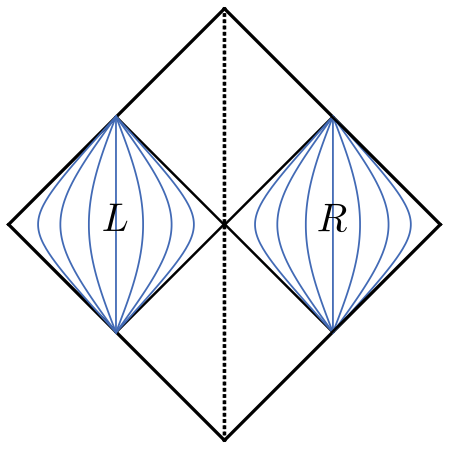
\includegraphics[width=0.4\textwidth]{cprindlermink}
\caption{Minkowski space in $1+1$ dimensions and the left and right Rindler wedges. Some accelerated worlines (lines of constant $\xi_L$ and $\xi_R$) have been drawn.}
\label{fig:cpminkrind}
\end{center}
\end{figure}

We will first look at QFT in Rindler space in $1+1$ dimensions, since it features many of the aspects that will be relevant in the discussion of Hawking radiation. By QFT in Rindler space we really mean the field quantisation as it would be carried out by eternally accelerated observers in Minkowski space. We shall see that such observers, when travelling through the Minkowski vacuum, will feel themselves immersed in a thermal bath of particles.\\

In light-cone coordinates $\bar u=t-x$ and $\bar v=t+x$, the line-element of $1+1$-dimensional Minkowski space is $ds^2=-d\bar u d\bar v$. In section~\ref{sec:cprindler} we constructed the Penrose diagram for Rindler space and we considered only the ``right Rindler wedge'': $\bar u<0$, $\bar v>0$. This corresponds to the region $R$ in Figure~\ref{fig:cpminkrind}. There also exists a left Rindler wedge $\bar u>0$, $\bar v<0$, denoted by $L$ in Figure~\ref{fig:cpminkrind}. In the right Rindler wedge, define the coordinates $\xi$ and $\eta$ via
\be\bal
t&=a^{-1}e^{a\xi}\sinh a\eta\\
x&=a^{-1}e^{a\xi}\cosh a\eta
\eal\ee
such that $-\infty<\xi,\eta<\infty$ and
\be
ds^2=e^{2a\xi}(-d\eta^2+d\xi^2).
\ee
The proper time measured by a Rindler observer (i.e. along a $\xi=const.$ line) is $\tau=e^{2a\xi}\eta$ if we synchronise it to $\tau=0$ as the observer passes the $x$-axis. Hence, the coordinate $\eta$ is a physical time-coordinate for the Rindler observer travelling at constant $\xi$: it ticks at a rate proportional to the observer's watch. %MB1: mention that t is not like that
 Now define the null coordinates $u=\eta-\xi$ and $v=\eta+\xi$, in terms of which the Rindler metric reads
\be
ds^2=-e^{2a\xi}dudv.
\ee
The relation between the Minkowski and Rindler null coordinates is
\be\bal
\bar u&=-a^{-1}e^{-au}\\
\bar v&=a^{-1}e^{av},\label{eq:minkrindrel}
\eal\ee
which implies that
\be\bal
\bar u\rightarrow0&\iff u\rightarrow+\infty\\
\bar v\rightarrow0&\iff v\rightarrow-\infty,
\eal\ee
as shown in Figure~\ref{fig:cpminkrind}. %MB1: DO THIS.
 Notice the analogy to the relationship between the null Eddington-Finkelstein coordinates (denoted above as $u,v$) and the Kruskal coordinates $U,V$~\eqref{eq:UV}: $U=-e^{-u/4M}$ and $V=e^{v/4M}$.\\%MB1: finish. This is precisely the same as~\eqref{eq:minkrindrel} modulo the  constant multiplier $a^{-1}$.
 
\input{rindlertable}

Analogous definitions can be made for coordinates that cover the left Rindler wedge. The coordinates and line elements for the left and right Rindler wedge are shown in table~\ref{tab:rindler}, where we've used subscripts to distinguish between the two wedges. \emph{In this section, Rindler coordinates without subscript always refer to the right wedge.}\\

In fact, the time coordinates $\eta_L=\eta_R=\tanh^{-1}(t/x)$ are exactly the same function of Minkowski coordinates --- they just take different ranges in $L$ and $R$. We can therefore drop the subscripts on $\eta$ completely, as long as we remember that $\eta<0$ corresponds to $L$ and $\eta>0$ to $R$. Lines of $\eta=const.$ then correspond to lines through the origin that extend over both $L$ and $R$. These lines are Cauchy surfaces for Minkowski spacetime. The vector $\partial_\eta$ is a timelike Killing vector \exercise in both $L$ and $R$, but it is future-pointing in $R$ and past-pointing in $L$. We now have three globally hyperbolic manifolds with global future-pointing timelike Killing vectors: Minkowski space with $\partial_t$, the left Rindler wedge with $-\partial_{\eta}$, and the right Rindler wedge with $\partial_{\eta}$. In each of these the canonical quantisation procedure outlined in the preceding section can be applied.\\

In Minkowski coordinates, the Klein-Gordon equation for the massless scalar field is $(-\partial_t^2+\partial_x^2)\phi=0$ and there exists a set of positive frequency ``Minkowski'' modes 
\be
f_k=\frac1{\sqrt{4\pi\omega_k}}\exp\left(-i\omega_kt+ikx\right)
\ee
with $\omega_k=|k|>0$. It is useful to make the distinction between ``left-moving'' and ``right-moving'' modes, which take a simple form in terms of Rindler light-cone coordinates:
\be\bal
f_k=
\begin{cases}
\displaystyle \frac1{\sqrt{4\pi\omega_k}}\exp\left(-i\omega_k\bar u\right)&\qquad k>0\qquad\text{``right-moving''}\\
\displaystyle \frac1{\sqrt{4\pi\omega_k}}\exp\left(-i\omega_k\bar v\right)&\qquad k<0\qquad\text{``left-moving''}.
\end{cases}
\eal\ee
The field expansion is
\be
\phi(x)=\sum_k a_kf_k(x)+a^\dagger_kf_k(x)^*
\ee
and the Minkowski vacuum is defined by $a_k|0_M\rangle=0\;\forall\;k$.\\

In $R$, the Klein-Gordon equation becomes $\Box\phi=e^{-2a\xi}(-\partial_\eta^2+\partial_\xi^2)\phi=0$, which admits plane wave solutions
\be
g^R_k=\frac1{\sqrt{4\pi\omega_k}}\exp\left(-i\omega_k\eta+ik\xi\right)\label{eq:rindmodesinR}
\ee
with $\omega_k=|k|>0$. These solutions are positive frequency with respect to $\partial_\eta$. Note that the functions $g^R_k$ as defined in~\eqref{eq:rindmodesinR} are only specified for $R\subset M$. An eternally accelerated observer in $R$ might use these modes to carry out the quantisation of the scalar field in $R$, which would lead to a field expansion
\be
\phi(x)=\sum_k b_kg^R_k(x)+b_k^\dagger g^R_k(x)^*
\ee
and a vacuum $b_k|0_R\rangle=0\;\forall\;k$. This vacuum has no (obvious) relation to the Minkowski vacuum and indeed pertains to an entirely different spacetime manifold (the Rindler wedge). However, we are interested in a different question here: how would an eternally accelerated observer travelling through Minkowski spacetime perceive the \emph{Minkowski} vacuum, i.e. the Poincar\'e-invariant ground state of Minkowski spacetime? In order to answer this, we need to decide what the appropriate positive frequency condition is for such an observer. The Killing vector $\partial_t$ is not natural to Rindler observers, since the coordinate $t$ is not proportional to the physical proper time measured by a Rindler observer's watch. Instead, we've seen above that the proper time of a Rindler observer is proportional to $\eta$. Hence, the vector $\partial_\eta$ is the natural Killing vector with respect to which a Rindler would measure frequencies and define a notion of positive frequency.\\

We need to extend our definition of the Rindler modes because as defined in~\eqref{eq:rindmodesinR} they are not specified on a Cauchy surface for $M$. For example, they are only defined on half of the Cauchy surface $\eta=0$ (for $x>0$). This is easily remedied by defining the \emph{global} modes $g^R_k$ as follows:
\be\bal
g^R_k=
\begin{cases}
\displaystyle\frac1{\sqrt{4\pi\omega_k}}\exp\left(-i\omega_k\eta+ik\xi\right)\qquad&\text{in } R\\
0&\text{in } L.
\end{cases}
\eal\ee
These modes are defined on an entire Cauchy surface (e.g. $\eta=0$). The set $\left\{g^R_k,g^{R*}_k\right\}$ does \emph{not} form complete basis for the functions on $M$ yet. For this reason, we also need to consider the positive-frequency modes in the left wedge $L$, which are associated with left-accelerating Rindler observers. These modes are given by
\be\bal
g^L_k=
\begin{cases}
\displaystyle\frac1{\sqrt{4\pi\omega_k}}\exp\left(+i\omega_k\eta+ik\xi\right)\qquad&\text{in } L\\
0&\text{in } R.
\end{cases}
\eal\ee
and are positive frequency with respect to $-\partial_\eta$ in $L$ (remembering that the \emph{future-pointing} timelike Killing vector in $L$ is $-\partial_\eta$). Taken together, the positive-frequency modes in $L$ and $R$ form a complete set, and so a field configuration $\phi(x)$ in Minkowski space may be expanded as
\be
\phi(x)=\sum_k b_kg^R_k(x)+c_kg^L_k(x)+{h.c.}\label{eq:fieldrindmodes}
\ee
where $h.c.$ denotes Hermitian conjugate. We can now ask: How many $R$-particles are expected to be seen in the Minkowski vaccum --- how many particles does the externally accelerated observer in the right wedge see? In other words, what is $\langle0_M|{}^RN_k|0_M\rangle$, where ${}^RN_k=b_k^\dagger b^{}_k$? To simplify things, we specialise our question to right-movers, for which $k>0\implies \omega=k$. We need the Bogoliubov coefficients
\be
g^R_\omega=\int_0^\infty d\omega' (A_{\omega\omega'}f_{\omega'}+B_{\omega\omega'}f_{\omega'}^*)\label{eq:bogrind}
\ee
where $f_{\omega'}=(4\pi\omega')^{-\frac12}\exp\left(-i\omega'\bar u\right)$. Notice the resemblance of this integral with the Fourier transform of $g^R_\omega$:
\be
g^R_{\omega}(\bar u)=\frac1{2\pi}\int_{-\infty}^\infty d\omega'e^{-i\omega'\bar u}\tilde g_\omega(\omega')\label{eq:ftrind}
\ee
where
\be
\tilde g_{\omega}(\omega')=\int_{-\infty}^\infty d\bar u\, e^{i\omega'\bar u}\,g^R_\omega(\bar u)
\ee
(for notational convenience we omit the superscript $R$ on the Fourier transform). Our strategy is now to massage~\eqref{eq:ftrind} into a form that allows us to write the Bogoliubov coefficients in~\eqref{eq:bogrind} in terms of the Fourier transform $\tilde g_\omega$. To that end, we split up the integral in~\eqref{eq:ftrind} as follows:
\be
g^R_\omega(\bar u)=\frac1{2\pi}\int_0^\infty d\omega'e^{-i\bar u\omega'}\tilde g_\omega(\omega')+\frac1{2\pi}\int_0^\infty d\omega'e^{i\bar u\omega'}\tilde g_\omega(-\omega').
\ee
We flipped the sign of the integration variable $\omega'\rightarrow-\omega'$ in the second term. Comparing with~\eqref{eq:bogrind}, we find
\be
A_{\omega\omega'}=\sqrt{\frac{\omega'}{\pi}}\tilde g_\omega(\omega')\quad\mand\quad B_{\omega\omega'}=\sqrt{\frac{\omega'}{\pi}}\tilde g_\omega(-\omega').\label{eq:bogft}
\ee
In order to find the Bogoliubov coefficients~\eqref{eq:bogft}, we don't actually need to evaluate the Fourier transforms. It is enough if we can relate $\tilde g_\omega(\omega')$ to $\tilde g_{\omega}(-\omega')$, since the additional condition $\mathbf{AA}^\dagger-\mathbf{BB}^\dagger=\mathbf 1$ then fixes $A_{\omega\omega'}$ and $B_{\omega\omega'}$ completely. To do so we prove the following claim:\\%MB1: JUSTIFY THIS STATEMENT

\noindent\textbf{Claim:} $\tilde g_\omega(-\omega')=-e^{-\pi\omega/a}\tilde g_\omega(\omega')$ if $\omega'>0$.\\

\noindent\textbf{Proof:} The integral defining $\tilde g_\omega$ uses $g^R_\omega$ in terms of $\bar u$. Since $u=-a^{-1}\ln(-a\bar u)$, the right-moving $R$-modes take the form
\be
g^R_\omega=
\begin{cases}
\displaystyle\frac1{\sqrt{4\pi\omega_k}}e^{-i\frac{\omega}{a}\ln(-a\overline u)}\qquad&\text{for } \bar u<0\\
0&\text{for } \bar u >0.
\end{cases}
\ee 
The function $\ln(-z)$ is multi-valued on the complex plane so we will give it a branch cut on the positive real axis. Then
\begin{figure}[t!]
\begin{center}
\includegraphics[width=0.75\textwidth]{contour}
\caption{The contour integral used in the evaluation of $g^R_\omega(-\omega')$ with a branch cut of $\ln(-z)$ on the positive real axis.}
\label{fig:contour}
\end{center}
\end{figure}
\be\bal
\tilde g_\omega(-\omega')&=\int_{-\infty}^\infty d\bar u\, e^{-i\omega'\bar u} g_\omega(\bar u)\\
&= \frac1{\sqrt{4\pi\omega}}\int_{-\infty}^0 d\bar u\, e^{-i\omega'\bar u}e^{-i\frac{\omega}{a}\ln(-a\overline u)}.
\eal\ee
Now we deform the path of integration, using the contour shown in Figure~\ref{fig:contour}. The contour is closed in the upper complex half-plane because the integral over the arc segment $\mathcal C$ then vanishes for $\omega'>0$ in the limit as the radius of the arc goes to infinity. In order to avoid the branch cut we choose $\gamma_2$ to lie just above the real axis by an infinitesimal amount $i\epsilon$ (which we send to zero at the end). Since the integrand has no poles inside the closed contour (i.e. it is holomorphic there), Cauchy's integral theorem implies
\be
0=\oint d\bar u\, e^{-i\omega'\bar u}e^{-i\frac{\omega}{a}\ln(-a\overline u)}=\left\{\int_{\gamma_1}+\int_{\gamma_2}+\int_{\mathcal C}\right\}d\bar u\, e^{-i\omega'\bar u}e^{-i\frac{\omega}{a}\ln(-a\overline u)}.\label{eq:cauchyint}
\ee
Strictly speaking, there is another contribution on the right hand side for the integral from $i\epsilon$ to $0$ (see Figure~\ref{fig:contour}), but this will vanish when we send $\epsilon$ to zero at the end so we can forget about it here. Since the integral over the arc $\mathcal C$ vanishes, it follows from~\eqref{eq:cauchyint} that $\int_{\gamma_1}=-\int_{\gamma_2}$, which implies
\be\bal
\tilde g_\omega(-\omega')&=- \frac1{\sqrt{4\pi\omega}}\int_{i\epsilon}^{\infty+i\epsilon} d\bar u\, e^{-i\omega'\bar u}e^{-i\frac{\omega}{a}\ln(-a\overline u)}\\
&=-\frac1{\sqrt{4\pi\omega}}\int_{-\infty-i\epsilon}^{-i\epsilon} d\bar u\, e^{i\omega'\bar u}e^{-i\frac{\omega}{a}\ln(a\overline u)}\qquad(\bar u\leftrightarrow-\bar u)\\
&=-\frac1{\sqrt{4\pi\omega}}\int_{-\infty}^0 d\bar u\, e^{i\omega'\bar u}e^{-i\frac{\omega}{a}\left[\ln(-a\overline u)-i\pi\right]}\qquad (\epsilon\rightarrow0)\\
&=-e^{-\pi\omega/a}\tilde g_\omega(\omega')
\eal\ee
as claimed.\qed\\

Hence we have $A_{\omega\omega'}=-e^{-\pi\omega/a}B_{\omega\omega'}$, which together with $|A_{\omega\omega}|^2-|B_{\omega\omega}|^2=1$ implies
\be
\langle0_M|{}^RN_\omega|0_M\rangle=(\mathbf B\mathbf B^\dagger)_{\omega\omega}=|B_{\omega\omega}|^2=\frac1{e^{2\pi\omega/a}-1}.
\ee
This corresponds to a \emph{Planck spectrum} with temperature $T=\frac{\hbar a}{2\pi k_B}$.\\ %MB1: mention Unruh detector calculation (NOTES). The interpretation of this result is that an eternally accelerating observer....

In fact, we can show more: the state $|0_M\rangle$ \emph{is} the thermal state with respect to the Rindler Hamiltonian $\hat H_{R}$, i.e. the Hamiltonian associated with a hypersurface $\eta=const.$ in the right Rindler wedge (in other words, $\hat H_R$ generates time-translations along $\partial_\eta$). Mathematically this statement is
\be
\text{Tr}_{L}\left(|0_M\rangle\langle0_M|\right)=\frac{e^{-\beta \hat H_R}}{\langle e^{-\beta\hat H_R}\rangle}
\ee
where $\beta=(k_bT)^{-1}=2\pi k_b/\hbar a$. To show this, it is convenient to introduce so-called \emph{Unruh modes}, which are positive frequency with respect to $\partial_t$, i.e. they are linear combinations of $f_k$-modes. The Unruh mode of frequency $k$ is defined as
\be
z_k=\frac1{\sqrt{2\sinh\omega\pi/a}}\left(e^{\pi\omega/2a}\,g^R_k+e^{-\pi\omega/2a}\,g^L_{-k}\right).
\ee
In order to form a complete set, they must be complemented by the modes
\be
z'_k=\frac1{\sqrt{2\sinh\omega\pi/a}}\left(e^{-\pi\omega/2a}\,g^R_{-k}+e^{\pi\omega/2a}\,g^L_k\right).
\ee
The modes $z_k$ and $z'_k$ together with their complex conjugates form a complete basis for functions on Minkowski space. Hence, the field can be equally well expanded in terms of them:
\be
\phi(x)=\sum_k d_kz_k(x)+d^{\,\prime}_kz'_k(x)+{h.c.}
\ee
Comparing this with~\eqref{eq:fieldrindmodes} we can read off
\be\bal
b_k&=\frac1{\sqrt{2\sinh\omega\pi/a}}\left(e^{\pi\omega/2a}d_k+e^{-\pi\omega/2a}d_{-k}^{\,\prime\,\dagger}\right)\\
c_k&=\frac1{\sqrt{2\sinh\omega\pi/a}}\left(e^{\pi\omega/2a}d^{\,\prime}_k+e^{-\pi\omega/2a}d_{-k}^{\,\dagger}\right)
\eal\ee
Since the Unruh modes are positive frequency with respect to $\partial_t$, the Minkowski vacuum satisfies $d^{}_k|0_M\rangle=d^{\,\prime}_k|0_M\rangle=0\;\forall\;k$. Now define the \emph{Rindler vacuum} $|0_{Rd}\rangle$ by $c_k|0_{Rd}\rangle=b_k|0_{Rd}\rangle=0\;\forall\;k$ and further the %MB1:
(unnormalised)
left- and right-wedge $n$-particle states
\be
\left|{}^Rn,k\right>=(b_k^\dagger)^n\left|0_{Rd}\right> \mand \left|{}^Ln,k\right>=(c_k^\dagger)^n\left|0_{Rd}\right>.
\ee
Then it can be shown that
\be
|0_M\rangle=\prod_k(\cosh\phi_k)^{-1}\sum_{n=0}^\infty e^{-n\pi\omega/a}\left|{}^Rn,k\right>\left|{}^Ln,k\right>
\ee
where $\phi_k$ is defined by $\tanh\phi_k=e^{-\pi\omega/a}$. This state is perfectly entangled between the left and right Rindler wedges: if a measurement is done in $R$ in which $n$ right-wedge particles are found, then we know with certainty that the post-measurement state has $n$ left-wedge particles. To find the state $\rho_R$ in $R$, we need to trace over the states in $L$ via the ``partial trace'' $\text{Tr}_L$. Defining $E_n=n\omega$, we obtain
\be\bal
\rho_R&=\text{Tr}_L\left|0_{M}\right>\left<0_M\right|
&=\sum_{n=0}^\infty\prod_k\frac{e^{-\beta E_n}}{\sum_{m=0}^\infty e^{-\beta E_m}}\left|{}^R n,k\right>\left<{}^R n,k\right|
&=\frac{e^{-\beta\hat H_{R}}}{\langle e^{-\beta\hat H_R}\rangle}
\eal\ee
as claimed above. This reveals something perhaps surprising about the Minkowski vacuum: it is not a local quantity at all, i.e. it is not a state of the form 
$$
(\text{vacuum at }x_1)\otimes(\text{vacuum at }x_2)\otimes(\text{vacuum at }x_3)\otimes\ldots$$ 
Instead, it is a highly entangled state whose fluctuations are correlated throughout spacetime.\\

The actual physical meaning of the results above may perhaps seem a bit obscure. We considered the quantisation of a quantum field ``appropriate to a Rindler observer'' in Minkowski space, which led us to conclude that a Rindler observer is immersed in a thermal bath of radiation. How convincing were our arguments for choosing some appropriate quantisation scheme? How would an eternally accelerated observer actually \emph{measure} the radiation? 
To put the results derived above on more solid grounds, Bill Unruh constructed a simple model of a detector (nowadays known as an Unruh-deWitt detector) and showed that an accelerated detector in Minkowski space behaves as if it were in a thermal bath of particles. This effect is known as the \emph{Unruh effect}. Hawking radiation, which we discuss next, is a phenomenon closely related to this effect.

\subsection{QFT in the spacetime of a spherical collapsing star: Hawking Radiation}

Consider the spacetime that corresponds to a spherically symmetric collapsing star, heavy enough to form a black hole. The Penrose diagram is shown in Figure~\ref{fig:collapsingstar}.  This is a curved spacetime that is globally hyperbolic (for instance $\scri^-$ is a Cauchy surface). Even though the Schwarzschild black hole solution is a static spacetime, the collapsing star spacetime is \emph{not}: the formation of the black hole involves complicated dynamics. However, the spacetime is approximately stationary in the far asymptotic past (i.e. near $\scri^-$) and in the far asymptotic future (i.e. near $\scri^+$). Therefore we can perform a second quantisation associated with stationary observers near $\scri^-$ (which leads to the so-called \emph{in}-vacuum), and a second quantisation associated with stationary observers near $\scri^+$. We can then ask the question we asked in the example of the ``sandwich spacetime'' above: will observers in the far future see particles in the $in$-vacuum?\\

The field expansion defining the $in$-vacuum can be constructed by specifying a complete set of positive-frequency modes on $\scri^-$. For the quantisation in the far future, it is not sufficient to define a complete set on $\scri^+$, because $\scri^+$ is not a Cauchy surface for the spacetime (for example, causal curves that end on the singularity never register on $\scri^+$). However, the surface $ H^+\cup\scri^+$ is a Cauchy surface, so we can quantise the field in the far future by specifying a complete set on it. Hence there will be three sets of modes:
\be\bal
f_i &: \text{positive frequency on }\scri^-\\
g_i&: \text{positive frequency on }\scri^+\text{ and zero on }H^+\\
h_i&: \text{positive frequency on }H^+\text{ and zero on }\scri^+.
\eal\ee
(Strictly speaking, there is no timelike Killing vector on $H^+$ --- recall that $\partial_t$ is null on the horizon --- so the term ``positive frequency'' is somewhat misleading there. However, the outcome of the calculation does not actually depend on the choice of modes $h_i$, so we can just choose an arbitrary set of modes on $H^+$ and declare those as the ``positive frequency'' modes, i.e. attach them to annihilation operators in the field expansion, as long as together with $g_i$ they form a complete set. For more detail, see Wald \S 14.3.) The set $\left\{f_i,f_i^*\right\}$ is complete. The sets $\left\{g_i,g_i^*\right\}$ and $\left\{h_i,h_i^*\right\}$ are not complete by themselves but together they form a complete set. We can expand the field in two ways:
\begin{figure}[t!]
\begin{center}
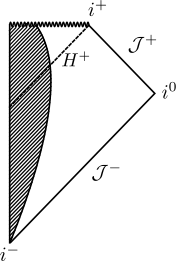
\includegraphics[width=0.25\textwidth]{collapsingstar}
\caption{Penrose diagram of the spherically symmetric collapsing star.}\label{fig:collapsingstar}
\end{center}
\end{figure}
\be
\phi(x)=\sum_i a_if_i(x)+{h.c.}=\sum_i b_ig_i(x)+c_ih_i(x)+{h.c.}
\ee
As before, to find out what observers at late times on $\scri^+$ see in the state $\left|0_{in}\right>$ defined by $a_i\left|0_{in}\right>=0\;\forall\;i$, we will evaluate $\left<N_i\right>=(\mathbf{BB}^\dagger)_{ii}$, for which we need the Bogoliubov coefficients in the expansion
\be
g_i=\sum_j A_{ij}f_j+B_{ij}f_j^*.\label{eq:gexpansion}
\ee

If we could find the exact solutions to the Klein-Gordon equation, this would be a fairly straight-forward task: once the positive-frequency solutions $g_i$ on $\scri^+$ are specified, we can do the analog of a Fourier transform to find their expansion in terms of $f_i$ and $f_i^*$ on $\scri^-$ (such an expansion always exists since $\left\{f_i,f_i^*\right\}$ is a complete set of functions) and read off the Bogoliubov coefficients. However, we will see in a moment that the Klein-Gordon equation is complicated in Schwarzschild spacetime, which prevents us from finding analytic solutions. Instead, we will ask: if a given solution to the Klein-Gordon equation is asymptotically positive-frequency at $\scri^+$, then what is its form at $\scri^-$? In other words, we will impose a boundary condition to the solution at $\scri^+$ and investigate what its corresponding form must be on $\scri^-$. This amounts to ``tracing back in time'' the solution from $\scri^+$ to $\scri^-$.\\

The metric of the Schwarschild black hole spacetime with coordinates $(t,r_*,\theta,\phi)$ reads
\be
ds^2=\sfac(-dt^2+dr_*^2)+r^2d\Omega_2^2.
\ee
We will also use the light-cone coordinates $u=t-r_*$ and $v=t+r_*$ below. Using the handy formula
\be
\Box=\nabla^\mu\nabla_\mu=\frac{1}{\sqrt{-g}}\partial_\mu\left(\sqrt{-g}g^{\mu\nu}\partial_\nu\right)
\ee
we can find the Klein-Gordon equation for the field $\phi(t,r_*,\theta,\phi)$. Expanding the solution in spherical harmonics $\phi(t,r_*,\theta,\phi)=\chi_l(r_*,t)Y_{lm}(\theta,\phi)$ we find%MB1: more detail on spherical harmonics
\be
\left[\partial_t^2-\partial_{r_*}^2+V_l(r_*)\right]\chi_l=0\label{eq:ssdiffeq}
\ee
where
\be
V_l(r_*)=\sfac\left[\frac{l(l+1)}{r^2}+\frac{2M}{r^3}\right].
\ee
Set $\chi_l(r_*,t)=e^{-i\omega t}R_{l\omega}(r_*)$ so that
\be
(\partial_{r_*}^2+\omega^2)R_{\omega l}=V_l R_{\omega l}.\label{eq:sseompot}
\ee
This equation can be cast into a form known as the \emph{confluent Heun equation}, whose solutions have been studied to some extent but are complicated. %MB1: proof?
We can gain some insight into the solutions by looking more closely at the potential $V_l(r_*)$. Both near the horizon $H^+$ $(r\rightarrow2M\iff r_*\rightarrow-\infty$) and near $\scri^\pm$  $(r\rightarrow\infty\iff r_*\rightarrow\infty$), the potential tends to zero --- it takes the form of a \emph{potential barrier}, as shown in Figure~\ref{fig:sspot}. Hence, if we consider how any particular solution to~\eqref{eq:sseompot} evolves in time, it will be partly transmitted and partly reflected as it comes in from $r_*=\infty$.\\

\begin{figure}[t!]
\begin{center}
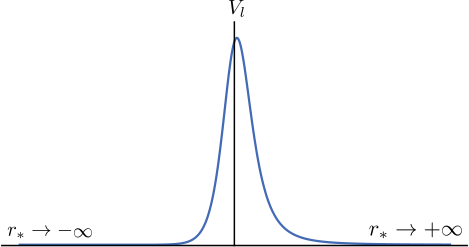
\includegraphics[width=0.75\textwidth]{sspot}
\caption{The potential $V_l$ as a function of $r_*$ (shown here for $l=1$).}
\label{fig:sspot}
\end{center}
\end{figure}

Near $\scri^\pm$, the solutions to~\eqref{eq:ssdiffeq} are just plane waves. The equivalent of right-moving and left-moving for a radial coordinate is outgoing and ingoing (corresponding, respectively, to $r_*$ increasing or decreasing with time) so we define ``early modes''
\be\bal
f_{lm\omega+}&=\frac1{\sqrt{2\pi\omega}}e^{-i\omega u}\frac{Y_{lm}}{r}\qquad\text{(outgoing)}\\
f_{lm\omega-}&=\frac1{\sqrt{2\pi\omega}}e^{-i\omega v}\frac{Y_{lm}}{r}\qquad\text{(ingoing)}
\eal\ee
at $\scri^-$, and ``late modes''
\be\bal
g_{lm\omega+}&=\frac1{\sqrt{2\pi\omega}}e^{-i\omega u}\frac{Y_{lm}}{r}\qquad\text{(outgoing)}\\
g_{lm\omega-}&=\frac1{\sqrt{2\pi\omega}}e^{-i\omega v}\frac{Y_{lm}}{r}\qquad\text{(ingoing)}
\eal\ee
at $\scri^+$. We will be interested mainly in ingoing early modes and outgoing late modes, so we will use the shorthand notation
\be\bal
f_{\omega}&\sim f_{lm\omega-}\\
g_{\omega}&\sim g_{lm\omega+}.
\eal\ee
We need to express $g_\omega$ in terms of $f^{}_{\omega'}$ and $f_{\omega'}^*$ on $\scri^-$. First, note that plane waves such as $g_\omega$ are in fact completely delocalised, i.e. they have support everywhere on $\scri^+$. However, using a superposition of such positive frequency plane waves, we can always construct a localised ``wave packet'' on $\scri^+$ (for example a Gaussian packet) and we can choose it to be peaked around some momentum $\omega_0$ and around some coordinate value $u_0$. Hence, when we speak of the ``outgoing mode at late times'' we really mean a linear combination of outgoing modes on $\scri^+$. Keeping this in mind, we phrase our argument below in terms $g_\omega$ for simplicity.\\

In order to find the expansion of the late mode in terms of early modes, we can trace the solution back in time. As the wave travels inwards from $\scri^+$ (toward decreasing values of $r_*$), it will encounter the potential barrier. One part of the wave, call it $g_\omega^{(r)}$, will be reflected and end up on $\scri^-$ with the same frequency $\omega$. This will correspond to a term of the form $A_{\omega\omega'}\propto\delta(\omega-\omega')$ in~\eqref{eq:gexpansion}. The remaining part $g_\omega^{(t)}$  of $g_\omega$ will be transmitted through the barrier and will enter the collapsing matter. In that region, the precise geometry of spacetime is unknown. However, since we are interested in a packet peaked at late times (i.e. large $u_0$) and at some finite frequency $\omega_0$, we know that the packet will be peaked at a very high frequency as it enters the collapsing matter due to the gravitational blueshift. This leads to an important simplification: the packet will obey the \emph{geometric optics approximation}, which means that $g_\omega$ takes the form $A(x) e^{i S(x)}$ where $A(x)$ is slowly varying compared to $S$. Substituting this into the Klein-Gordon equation gives $\nabla_\mu S\nabla^\mu S=0$, which means that surfaces of constant phase are null. Given a wave, we can therefore trace its surfaces of constant phase back in time by following null geodesics.\\

\begin{figure}[t!]
\begin{center}
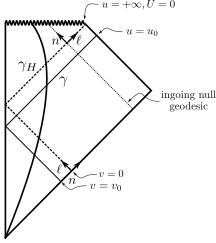
\includegraphics[width=0.5\textwidth]{collapsingstarhawkrad}
\caption{The BLA.}
\label{fig:sshawkingdiag}
\end{center}
\end{figure}

Consider tracing back the wave along a particular null geodesic $\gamma$ which starts off at some $u=u_0$ at $\scri^+$ and hits $\scri^-$ at $v=v_0$. as in Figure~\ref{fig:sshawkingdiag}. We denote by $\gamma_H$ a null generator of the horizon $H^+$, which has been extended into the past until it hits $\scri^-$ at some value of $v$. We may set this value to $v=0$ without loss of generality, since the spacetime is invariant under shifts $v\rightarrow v+c$. In that case we have $v_0<0$ for the geodesic $\gamma$. Let $n$ be a connecting vector between the two curves as shown in Figure~\ref{fig:sshawkingdiag}. Fix its normalisation by requiring $n.\ell=-1$, where $\ell$ is a generator of the Killing horizon $H^+$. Near the horizon, the Kruskal coordinate $U=-e^{-\kappa u}$ is an affine distance along $n$ and we can use it to measure the distance between $\gamma $ and $\gamma_H$~\eqref{eq:UV}. In order to find the form of the wave at $\scri^-$, we need to understand how the affine distance along the connecting vector $n$ will change by the time $\gamma$ reaches $\scri^-$. At $\scri^-$, the coordinate $v$ is an affine parameter along the null geodesic integral curves of $n$. If $U_0=0$ (corresponding to $u_0=\infty$) then the affine distance is zero at $\scri^-$. Hence we can expand the affine distance between $\gamma$ and $\gamma_H$ at $\scri^-$ in powers of $U_0$: $v=cU_0+\mathcal O(U_0^2)$ for some constant $c>0$ (since $U,v<0$).  Using $u=-\kappa^{-1}\ln(-U)=-\kappa^{-1}\ln(-c v)$, we can conclude that if a mode takes the form $g_\omega\sim e^{-i\omega u}$ on $\scri^+$, the transmitted part $g_\omega^{(t)}$ on $\scri^-$ will take the form
\be
g^{(t)}_\omega\sim
\begin{cases}
e^{i\frac{\omega}{\kappa}\ln(-v)} \qquad&\text{for}\quad v<0\\
0 &\text{for}\quad v>0
\end{cases}
\ee
up to a constant phase. This is exactly analogous to the Rindler modes in the previous section, with $\kappa\leftrightarrow a$. We have $A_{\omega\omega'}=e^{-\pi\omega/\kappa}B_{\omega\omega'}$ and therefore
\be
\left< N_\omega\right>\propto\frac{1}{e^{\hbar\omega/k_BT}-1}
\ee
where the \emph{Hawking temperature} is given by $T=\frac{\hbar\kappa}{2\pi k_B}$. Since this temperature is inversely proportional to the mass, the black hole heats up as it evaporates.
\end{document}


%%%%%%%%%%%%%%%%%%%%%%%%%%%%%%%%%%%%%%%%%%
%%%%%%				       END OF DOCUMENT			 	 %%%%%%
%%%%%%%%%%%%%%%%%%%%%%%%%%%%%%%%%%%%%%%%%%




\section{My BH calculation}
Take $\gamma$ to be a (null geodesic) generator of the horizon. It is affinely parametrised by virtue of being a generator. Let $\ell$ be a tangent vector to the horizon at some point $p$ outside the matter. Consider at $p$ a future-directed null vector $n$ directed radially inwards such that $n.\ell\neq0$. For convenience set $n.\ell=-1$. Then $-\epsilon n$ connects $p$ with a point $p_\epsilon$ on a surface of constant phase $S$ outside of the horizon. What we mean by this is: if we follow the integral curve of $n$ parameter-distance $\lambda$  If we parallel-transport $n$ and $l$ back in time along $\gamma$, the points $p_\epsilon$ trace out a curve $\gamma_\epsilon$.


%\noindent \textsf{UNDER CONSTRUCTION.}



